\documentclass
[
    paper = a4,
    pagesize,
    12 pt,
    oneside,                       % Chose ›oneside‹ for digital version, ›twoside‹ for printed version.
    open = right,
    DIV = calc,
    BCOR = 0 mm,                   % Binding correction. Only necessary for printed version. Depends on actual binding.
    bibtotoc
]
{scrbook}

% Do not change the following commands.
\newcommand*{\printTitle}{}
\newcommand*{\printAuthor}{}
\newcommand*{\printDateOfBirth}{}
\newcommand*{\printPlaceOfBirth}{}
\newcommand*{\printSubject}{}
\newcommand*{\myTitle}[1]{\renewcommand*{\printTitle}{#1}}
\newcommand*{\myName}[1]{\renewcommand*{\printAuthor}{#1}}
\newcommand*{\myDateOfBirth}[1]{\renewcommand*{\printDateOfBirth}{#1}}
\newcommand*{\myPlaceOfBirth}[1]{\renewcommand*{\printPlaceOfBirth}{#1}}
\newcommand*{\mySubject}[1]{\renewcommand*{\printSubject}{#1}}

\myTitle{High-level Visualization of Graph Algorithms}  % Change!
\myName{Julius Milian Severin}  % Change!
\myDateOfBirth{March~12, 1995}  % Change!
\myPlaceOfBirth{Berlin, Germany}  % Change!
\mySubject{{Graph Algorithms}{Visualization}}  % Change!

\usepackage[utf8]{inputenc}
\usepackage[T1]{fontenc}
\usepackage[english]{babel}

\usepackage{graphicx}

\graphicspath{{Images/}}

\usepackage{pgf}

\usepackage							% Microtypography tuning.
[
	protrusion = true,
	expansion = false,
	tracking = true,
	kerning = true,
	spacing = false,
	babel = true
]
{microtype}							% http://ctan.mirrorcatalogs.com/macros/latex/contrib/microtype/microtype.pdf

\SetTracking[unit = space]{font = */*/*/sc/*}{25}   % Adjust kerning for small caps.

\SetExtraKerning[unit = space]		% Adjusted kerning for certain characters.
{
	font = */*/*/*/*
}
{
	: = {100, },
	; = {100, },
	? = {150, 150},
	! = {150, 150},
	: = {250, },
	; = {150, },
	? = {250, 250},
	! = {250, 250},
	» = { , -200},
	« = {-200, },
	› = { , -200},
	‹ = {-200, },
	– = {200, 250},
	— = {200, 250},
	@ = {200, 200}
}

\usepackage{booktabs}
\usepackage{breakurl}
\usepackage{emptypage}

\usepackage[bottom]{footmisc}
\usepackage{remreset}

\makeatletter
    \@removefromreset{footnote}{chapter}
\makeatother

\renewcommand*{\footnoterule}{\rule{0 pt}{0 pt}}
\deffootnote[1.2 em]{1.2 em}{0 em}{\makebox[1.4 em][l]{\textbf{\thefootnotemark}}}

\usepackage{xparse}

\DeclareDocumentCommand{\myfootnote}{o o o m}
{%
    \IfNoValueTF{#1}%
    {%
        \footnote{#4}%
    }%
    {%
        \IfNoValueTF{#2}%
        {%
            \kern #1 em\footnote{#4}%
        }%
        {%
            \IfNoValueTF{#3}%
            {%
                \kern #1 em\footnote{#4}\kern #2 em%
            }%
            {%
                \kern #1 em\footnote[#3]{#4}\kern #2 em%
            }%
        }%
    }%
}

\usepackage{titlesec}

\titleformat{\chapter}
    {\normalfont\rmfamily\huge\bfseries}
    {\thechapter}{1 em}{}

\titleformat{\section}
    {\normalfont\rmfamily\Large\bfseries}
    {\thesection}{1 em}{}

\titleformat{\subsection}
    {\normalfont\rmfamily\large\bfseries}
    {\thesubsection}{1 em}{}

\titleformat{\subsubsection}
    {\normalfont\rmfamily\normalsize\bfseries}
    {\subsubsectionname}{1 em}{}


\pagestyle{headings}

\usepackage{amsmath}
\usepackage{amssymb}
\usepackage{amsfonts}
%\usepackage{upgreek}               % Use if you want to use upright lowercase and italic upercase greek letters.
%\usepackage{dsfont}                % Use if you want to use special symbols.

%\usepackage[printonlyused]{acronym} % Use if you want to have acronyms. http://mirror.hmc.edu/ctan/macros/latex/contrib/acronym/acronym.pdf

%\usepackage{pifont}				% Special symbols.
%\usepackage{fourier-orns}			% More special symbols.
\usepackage{lettrine}

\usepackage{enumitem}
\usepackage
[
	format = plain,
	textfont = {sf, footnotesize},
	labelfont = {sf, bf}
]
{caption}[2008/08/24]
\usepackage{subcaption}				% For using sub-figures.

\usepackage
[
    algo2e,
    ruled,
    vlined,
    linesnumbered,
    algochapter
]
{algorithm2e}

\SetAlCapFnt{\sffamily\footnotesize}
\SetAlCapNameFnt{\sffamily\footnotesize}

\usepackage[numbers]{natbib}

\makeatletter
    \def\NAT@spacechar{~}% NEW
\makeatother

\definecolor{darkblue}{rgb}{0, 0, 0.5}

\usepackage
[
	bookmarks = true,
	bookmarksopen = false,
	bookmarksnumbered = true,
	pdfstartpage = 1,
	pdftitle = {{\printTitle}},
	pdfauthor = {{\printAuthor}},
	pdfsubject = {{\printSubject}},
	backref = page,
	breaklinks = true,
	colorlinks = true,
	linkcolor = darkblue,
	anchorcolor = darkblue,
	citecolor = darkblue,
	filecolor = darkblue,
	menucolor = darkblue,
	pagecolor = darkblue,
	urlcolor = darkblue
]

\usepackage{hyperref}


\renewcommand*{\backref}[1]{}
\renewcommand*{\backrefalt}[4]
{
    \ifcase #1
        Not cited.
    \or
        \footnotesize (Cited on page #2.)
    \else
        \footnotesize (Cited on pages #2.)
    \fi
}

\usepackage{cleveref}

\begin{document}




\begin{document}


\frontmatter
% Title Page
\thispagestyle{empty}
\begin{center}
    {\Huge \textbf{\printTitle}}\\[7 ex]
    {\Large\textsc{Bachelor Thesis}}\\[4 ex]    
    {\large
        to attain the scientific degree\\[4 ex]
        \textbf{Bachelor of Science}
    }
    \vfill
    \includegraphics[width = 8 cm]{HPI_logo.pdf}\\[8 ex]
    \begin{tabular}{l}
        handed in by \textbf{\printAuthor}\\[1.1 ex]
        born \printDateOfBirth, in \printPlaceOfBirth\\[3 ex]
        \textbf{Advisor:} Prof.~Dr.~Tobias Friedrich\\[9 ex]
    \end{tabular}
    
    Potsdam, \today
\end{center}

% Abstract
\chapter*{}
\addcontentsline{toc}{chapter}{Abstract}
\thispagestyle{empty}

\begin{center}
    \large \textbf{Abstract}
\end{center}

Developing an algorithm is an iterative process.
Therefore an understanding of the different approches is important.
Furthermore, as the algorithm becomes more complex, it may come to different results than expected, when running on real data.

This thesis deals with those issues on the example of shortest path algorithm on tiled map data.
Therefore, multiple ways of visualizing a shortest path algorithm with respect of this specific class of algorithms are introduced.
Using those methods we were able to archieve a better understanding of the algorithms and built a powerful basis for discussions.
In addition we enabled the researchers to find the missbehaviour more easily.

\chapter*{}
\addcontentsline{toc}{chapter}{Zusammenfassung}
\thispagestyle{empty}

\begin{center}
    \large \textbf{Zusammenfassung}
\end{center}

Das Entwickeln eines Algorithmusses ist ein iterativer Prozess.
Daher ist es wichitg, dass alle Beteiligten, die verschiedenen Ansätze verstehen.
Ausserdem kann es mit wachsender Komplexität des Algoithmus dazu kommen, dass sich der Algorithmus auf echten Daten anders verhalten als gedacht.
Das finden der Ursache kann ein äußerst komplexes Verfahren sein.

In der folgenden Arbeit erklären wir, wie wir die Entwicklung eines Algorithmus zum finden kürzester Wege durch eine Visualisierung untersützt haben.
Dabei gehen wir auf die Probleme ein, die wir wärend der Entwicklung der Visualisierung lösen mussten.


% Table of Contents
\renewcommand*{\listfigurename}{\normalfont\rmfamily\Large\bfseries List of Figures}
\renewcommand*{\listtablename}{\normalfont\rmfamily\Large\bfseries List of Tables}
\pdfbookmark{\contentsname}{toc}
\microtypesetup{protrusion = false}
    \tableofcontents
    \begingroup
    \let\clearpage\relax
    \listoffigures                  % Comment out if necessary.
    \listoftables                   % Comment out if necessary.
    \endgroup
\microtypesetup{protrusion = true}


\mainmatter
\chapter{Introduction} \label{introduction}
Graphs are a common structure in computer science.
Therefore developing more efficient graph algorithms plays a big role in algorithm engineering.
During the process of development knowing how the algorithm behaves is really important.
Firstly developing an algorithm is an iterative process it is fundamental to communicate about the different approaches and therefore create an understanding of them in the whole team.
Furthermore, the developed algorithms can become quite complex and therefore the idea of how the algorithms should behave and the way they actually behave on real graph data can diverge quite a lot.
\par
As the eyes are a fast way to access information a good way to achieve this understanding is to visualize the progress of the algorithm.
Though there are many tools for visualizing graphs, there is still a lack of algorithm visualization tools.
Therefore writing an own visualization that fits one's needs might be necessary.
In the following, we will describe the process of developing a sensemaking visualization the example of a shortest path algorithm. The algorithm was developed on a geographical tiled road network with the special requirement to reduce the amount of tile-accesses during the algorithm.


\chapter{Preliminaries} \label{questions}

In this chapter, we will first introduce the algorithm framework, that the visualization is going to display.
Then, we will touch upon the graph data the framework is running on.
After all, the characteristics of the visualization are presented.
The implementation of those characteristics is then discussed in \cref{main}.


\section{Problem Specification} \label{specification}
\todo{2 Abschnitte}
\subsection{The algorithm framework}

The visualization we built has the purpose of visualizing a framework for shortest path algorithms.
A shortest path algorithm, in general, has the goal to find the path with the lowest summed weight from a given start node to a target node in a weighted graph.

The baseline of the framework is Dijkstra's algorithm and its improvement, the A*-algorithm.
Dijkstra's algorithm starts at the start node wherefrom it adds its neighbors to a priority queue that orders the elements by their distance to the start node.
In each iteration, the node with the highest priority (smallest distance) is removed from the queue and its neighbors are added to the queue, when not already inserted.
Whenever the node that is going to be removed from the queue is the target node, the shortest path is found.
This results in a uniform spreading around the start node.\\

The A*-algorithm generally adopts this strategy.
To make the algorithm more target oriented, the queue of the A*-algorithm is ordered not only by the distance to the start node but also by the distance to the target node.
Thereby nodes presumably closer to the target get expanded
first.
This leads to a more target oriented spreading.\\

At this point, it is important to notice, that both algorithms create a coherent area of processed nodes.

\subsection{The graph}

The underlying graph of the framework is a road network.
Therefore every node has given coordinates that refer to a certain position on the Earth, the edges are directed and the weight of an edge can be calculated using its speed and its length.
Special about the graph is, that it is based on the Navigation Data Standart (NDS).
Based on the NDS the graph is split into tiles according to a geographical grid.

This impacts the algorithms in so far, that accessing tiles becomes the major effort on runtime, as the tiles are encrypted and compressed.
Hence the algorithm framework should access as little tiles as possible.
As the framework is developed for portable devices, the framework has access to the so-called cache, a fast storage with limited size.
Since tiles can be stored in the cache, accessing a tile is only costly whenever it is not in the cache.
Due to the limited size of the cache, loading a tile requires removing another, as soon as the cache is full.


\section{Basic Elements} \label{graph}

In the corresponding section in \cref{main} we are going to introduce the representations of basic elements of the graph.
We will discuss how to represent nodes, edges, and tiles in a meaningful way.
For the Nodes, we also had to start thinking about how to arrange them on the screen, or rather discuss how to map the coordinates on the spherical Earth onto a plane.
For the edges, a special challenge was to find a way to integrate the the length and the speed in the representation.


\section{Displaying the Algorithm}

In \cref{algorithm} we will describe how we built the foundation of the visualization.
With this foundation, we will then explain how we brought in the cache and added multiple features for a better accessibility of information.


\subsection{Basics}

In the corresponding \cref{basic} we are going to describe how we have combined the elements from \cref{graph} to build a basic visualization.
The main challenge here was how we could transform a static graph in a moving visualization that outlines the changing states of the graph during the ongoing algorithms of the framework.


\subsection{Visualizing the Cache} \label{pre_cache}


Based on the basic visualization build in \cref{basic} we were able to figure out how to make information about the state of the cache comprehensible.
Then we will explain how we achieved that it is possible to see how well a specific version of the framework performs regarding to the amount of tile loads, at any point of the visualization.


\section{Compare algorithms}

To see a progress in the development and examine an iteration of the framework is necessary to compare different versions of the framework based on the visualization.
After discussing the strategy of just putting two visualizations next to each other we are going to introduce alternative ways for comparing algorithms.


\section{Miscellaneous}

Based on the developed high-level visualization, we will introduce additional features we added for a better accessibility of information.


\chapter{Building the Visualization} \label{main}

In this chapter, we will solve the problems introduced in \cref{problem}.
This will happen in the same structure as they have been suggested.


\section{Basic Elements} \label{graph}

\paragraph{Nodes}
Mapping coordinates of the spherical Earth to a plane is an extensively discussed topic, as it is needed for geographical maps and has its origin in the late 7th millennium BCE
%\cite{wiki:cartography}
.
For our visualization, we considered two known projections.

Firstly the Mercator projection that is one of the most common projections, as it is used for most world maps and is also used by big map providers as Google maps
%\cite{google_maps}
 and was originally developed for nautical cartography in the 16th century
 %\cite{mercator}
 .
The other method is the Equirectangular projection which suggests itself due to its simplicity.
The Mercator projection firstly maps the Earth on a plane by using the longitude as horizontal coordinate and the latitude as the vertical coordinate.
As the geographical distance between the longitudes shrinks the more the latitudes get closer to the poles, the projection would now be distorted in those areas.
To prevent this effect the Mercator projection stretches the map vertically in the affected areas.

The Equirectangular is also known as unprojected map
%\cite{equirectangular}
.
This is because it does only use the longitude and the latitude as coordinates and does nothing else.

\begin{figure}[H]
    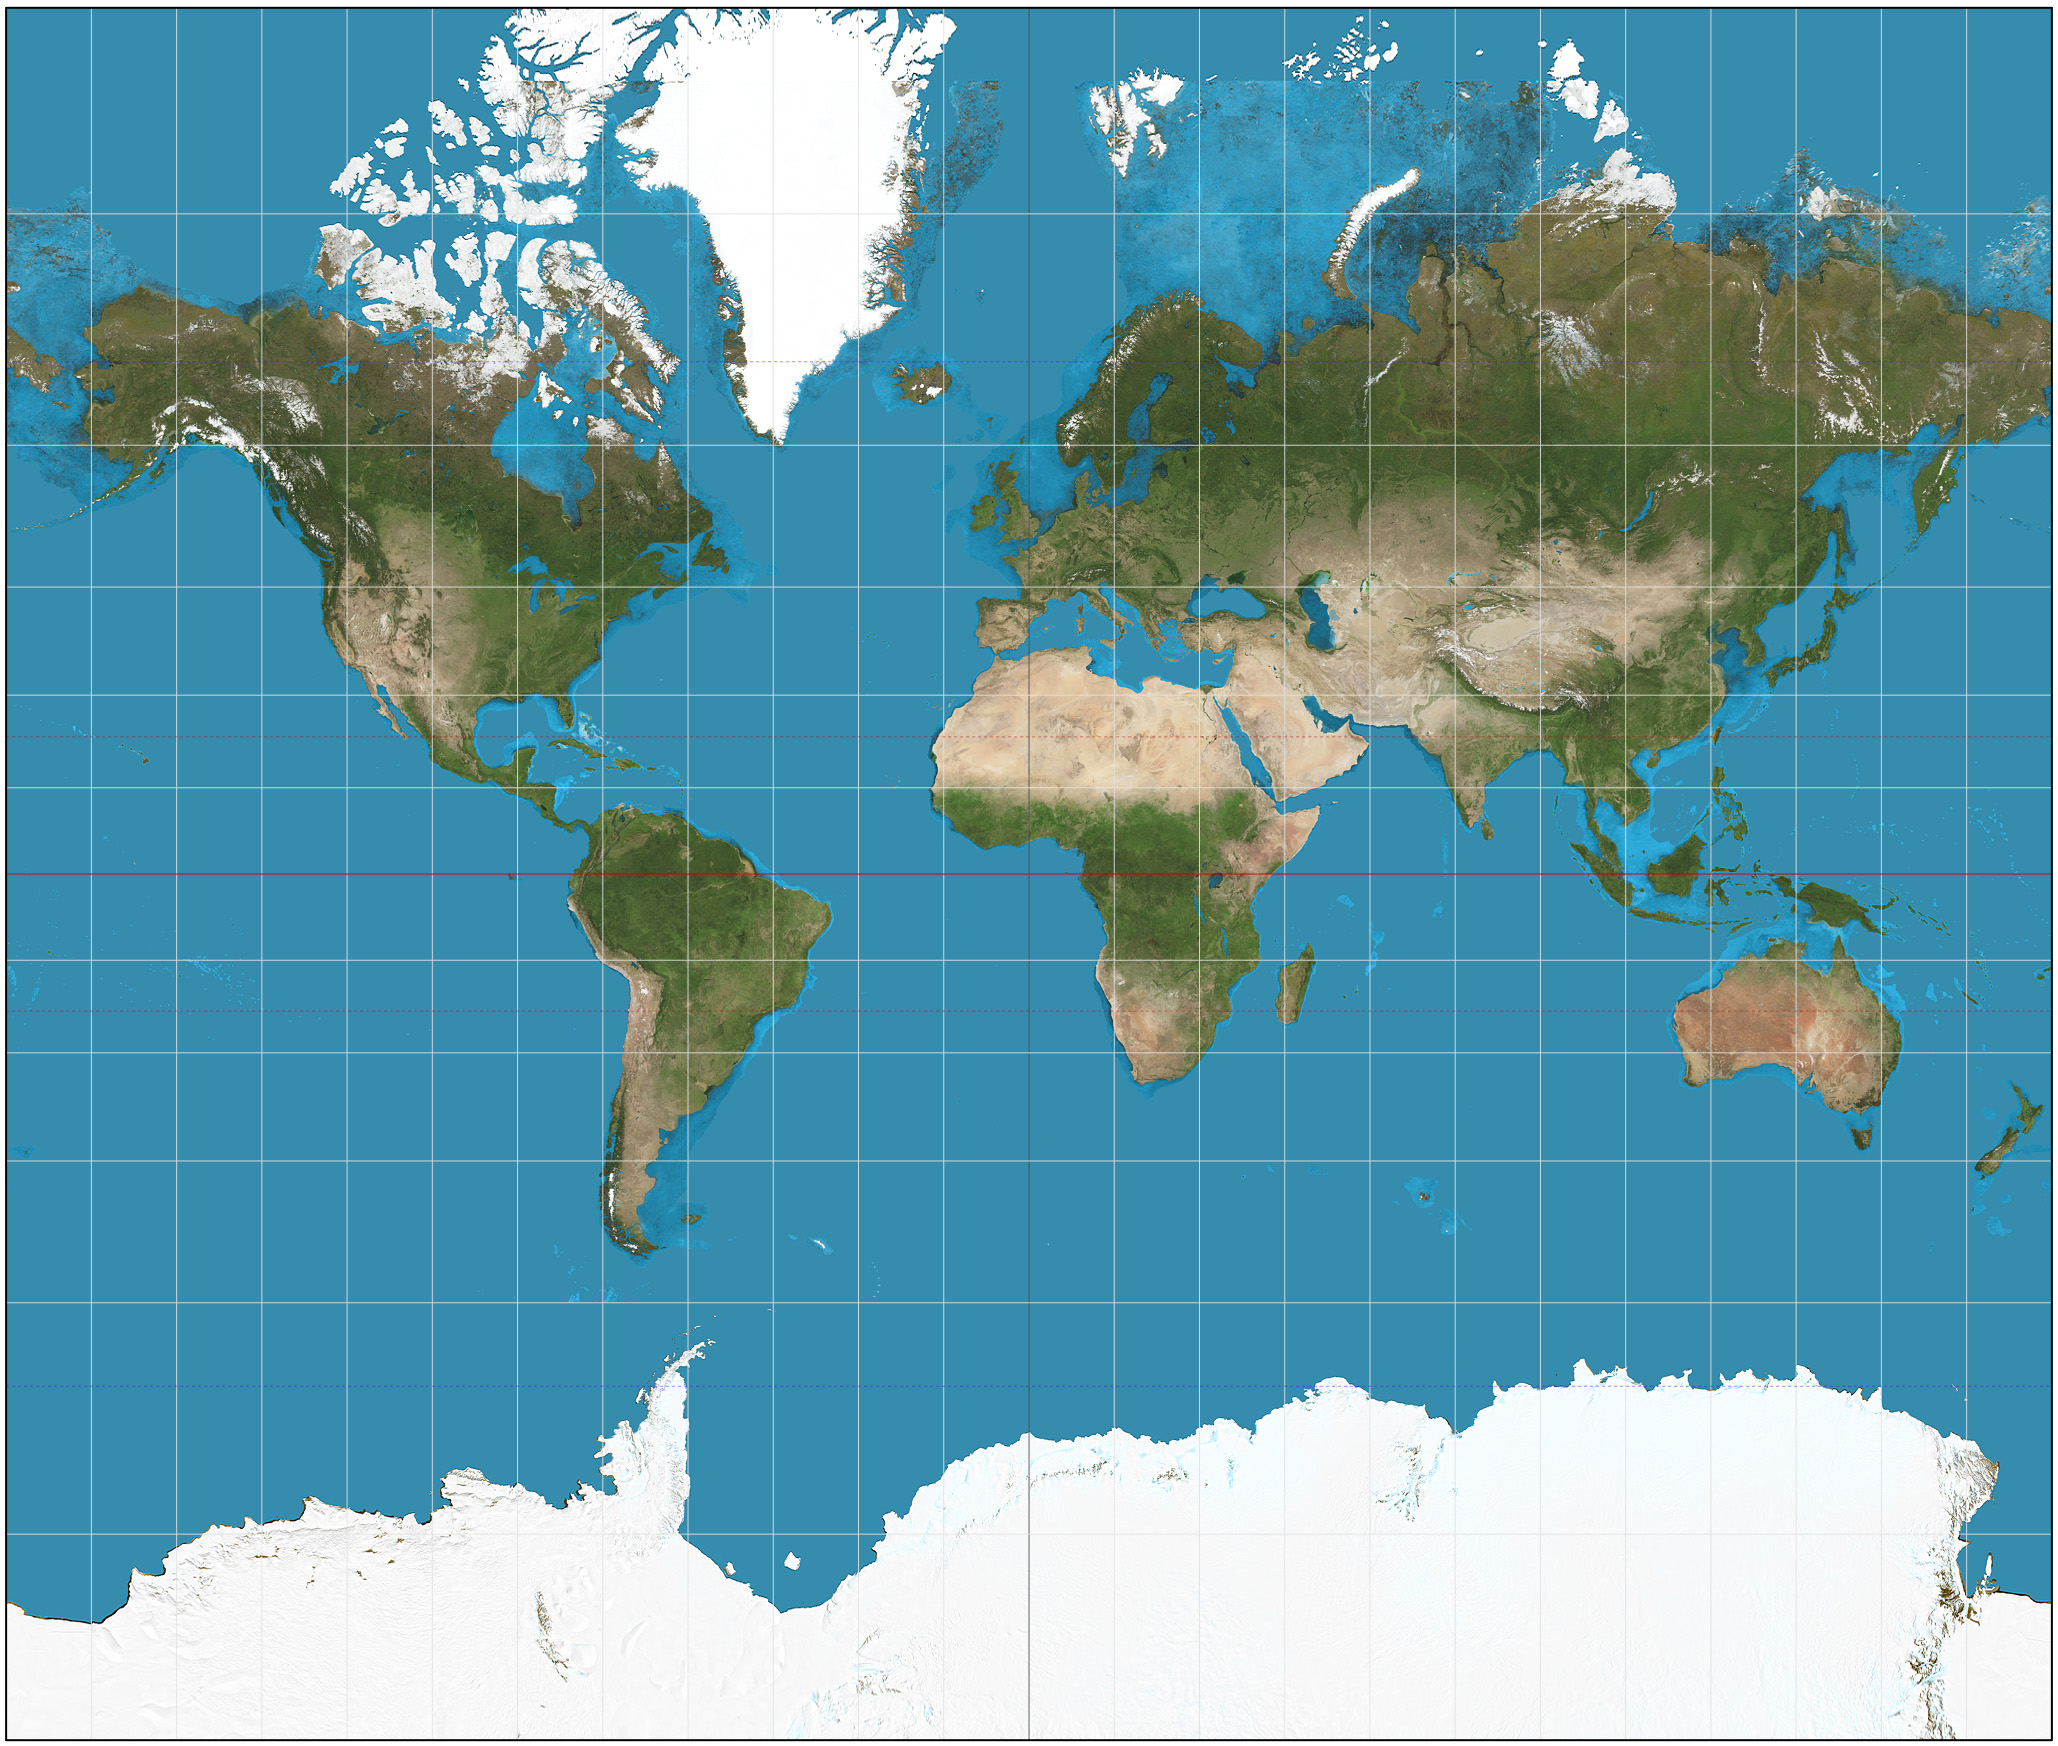
\includegraphics[width=.5\textwidth]{Images/Mercator_projection_SW.jpg}
    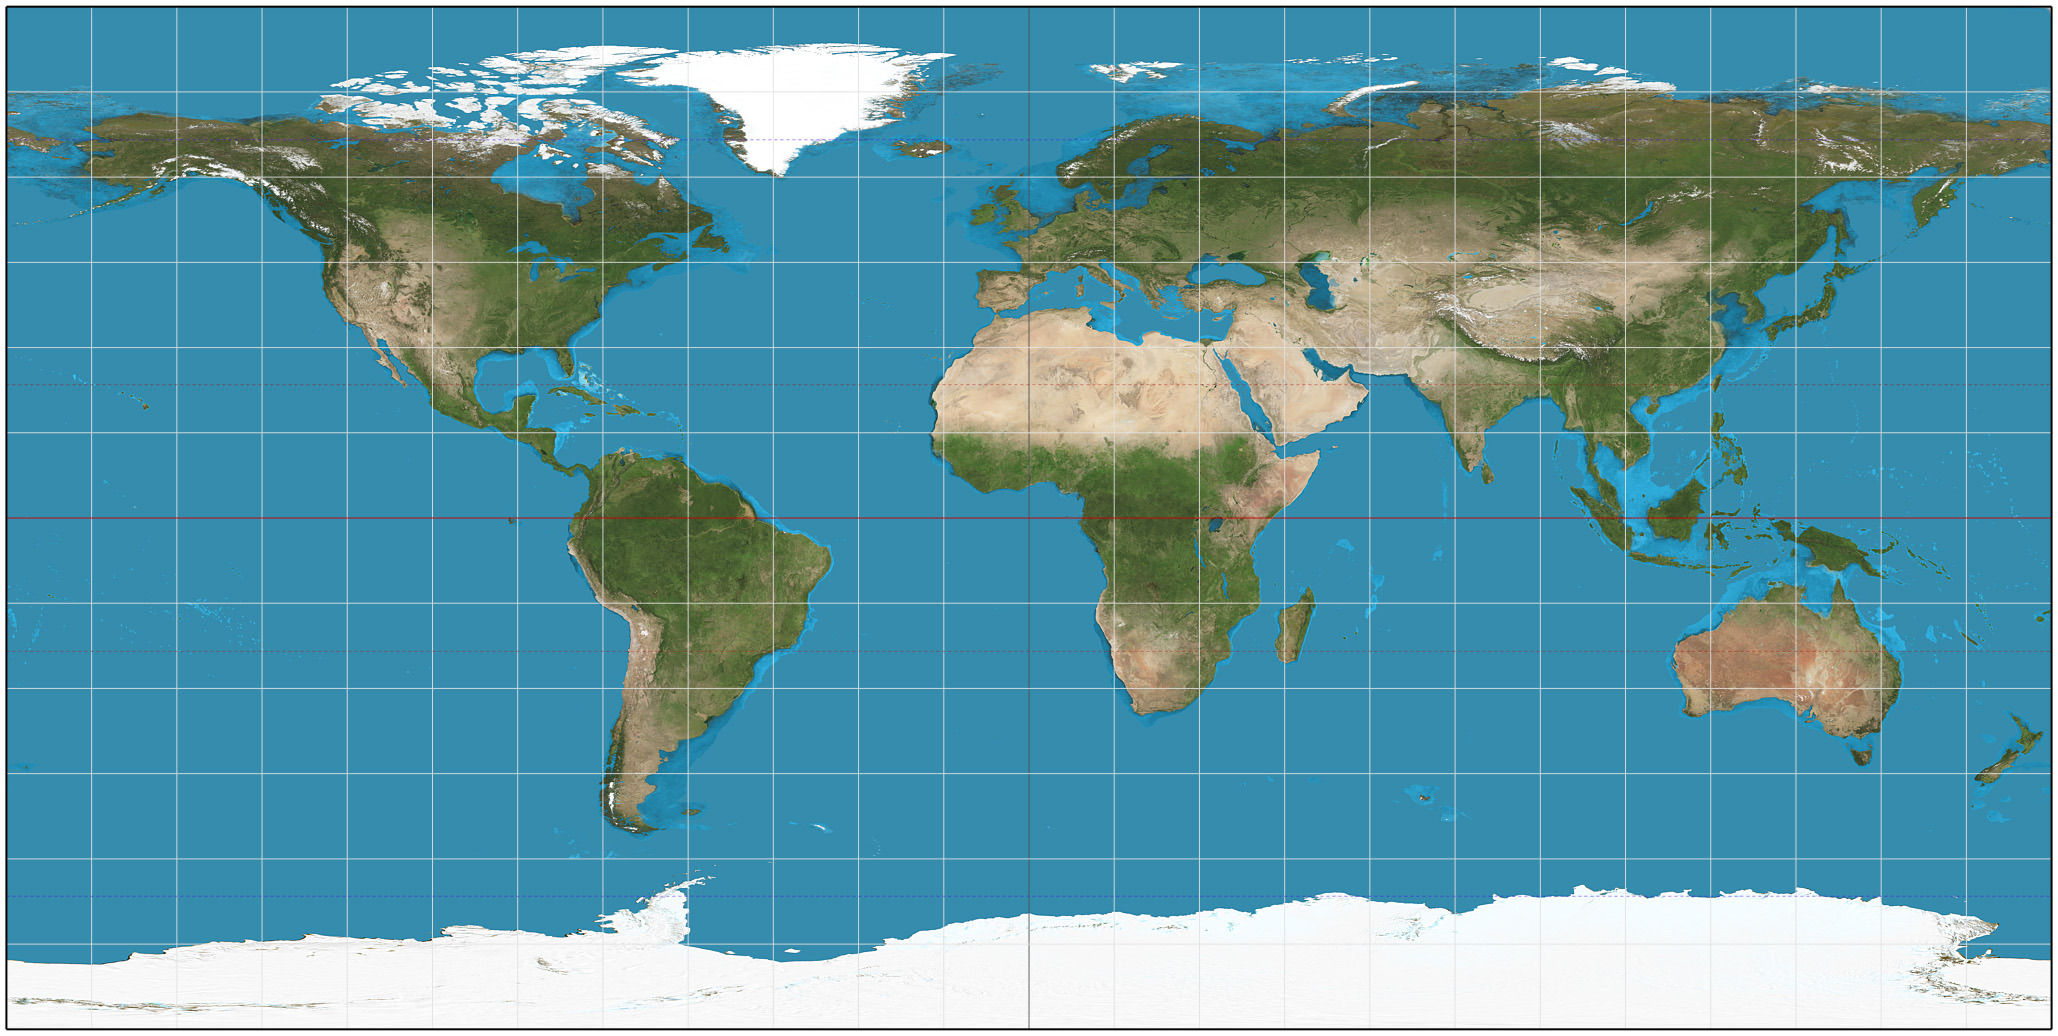
\includegraphics[width=.5\textwidth]{Images/Equirectangular_projection_SW.jpg}
\caption[]{A map of the Earth mapped by the Mercator projection(left) and the Equirectangular projection(right).}
\label{fig:projections}
\end{figure}

In \cref{fig:projections} we can see, what we already described before.
In contrast to the Equirectangular projection on the right that looks quite swaged near the poles, the Mercator projection on the left stretches vertically in those parts, which leads to a much more natural looking map.

Nevertheless, the Equirectangular projection has the huge benefit, that we can use the given coordinates without any additional calculations.
For the Mercator projection, we would have to apply a formula to each coordinate we would like to display.
Therefore, and due to the fact that the effect of the Mercator projection is quite low in most areas and particularly those that we are going to display, we decided to use the Equirectangular projection for further work.

\par For the representation of nodes circles are a common element and widely seen in graph visualizations.
Therefore, this was the first representation we considered for our visualization.
As those visualizations are mostly used for smaller graphs, mostly used to explain the basic concepts of an algorithm and we were going to display graphs with millions of nodes, we had to reconsider this representation of nodes.
We know that at the end of every edge is exactly one node.
Hence we can clearly identify every node, as long as the node is connected to any other edge.
Therefore we decided to not use any additional representation nodes to the visualization, as they did not add any value to it and only made the visualization more crowded.
Not specifically displaying the nodes, we missed out all the nodes, that do not have any neighbors.
But how to proceed with those remaining nodes?
As the only way for those nodes to play a role during our algorithm would be to be the start or the target node, we decided that the absence of those nodes would be reasonable and furthermore improve the clarity of our visualization.


\paragraph{Edges}

The first thing that comes to mind, when thinking about drawing edges, which is also widely seen in graph visualizations, is to represent them by straight lines.
This was also the approach we adopted.
The lines had the huge benefit that they did not add any bigger performance costs.
The length of the edges is in general reflected by the lines in most cases.
However, we need to respect, that it is possible, that the linear distance of two nodes, which is displayed by the linear representation, can diverge quite a lot to the length of the edge in some cases.
In addition, as we decided to use the Equirectangular projection, the lines are distorted horizontally dependent on their distance to the poles.

In order to represent the speed of an edge as well we came up with coloring the edges according to their speed, that can be used optionally.
We used the HSV color space because it provides an easy way for fluent color transitions.
Thereby we achieved a seamless color scheme that colors edges with a speed of 0 km/h in red, those with a speed of about 60 km/h in yellow and the fastest edges with a speed of 120 km/h and more in green.
Using this color scheme we would be able to outline edges with a speed of 240 km/h without any issues in understandability.


\paragraph{Tiles}
When we started visualizing the tiles, we first tried to get along without adding any new element.
Therefore we showed all edges of the tile in the background in gray as soon as the tile was accessed.
Later we figured out another way to display the tiles, as it was only possible to distinguish tiles at the outer graph.
By simply using rectangles to outline the tiles it was then possible to differentiate tiles at every part of the graph.
Due to the Equirectangular projection, all those rectangles have the same size and therefore the rectangles can be displayed without bigger costs in performance.


\section{Displaying the Algorithm} \label{algorithm}

In this section, we are going to outline how we used the elements, introduced in \cref{graph} for displaying how the graph evolves during the ongoing algorithms of the framework.

\subsection{Basics} \label{basic}

\paragraph{Combining the Elements}
A basic edge-based visualization starts with an empty space and then one edge after another is added as they have been passed by the framework.
For now, we assume displaying the right section of the graph is not a problem.
We will come back to this topic later in this section.

\todo{Schritt 3 und 4 eines Algorithmusses + farben}
\begin{figure}[H]
    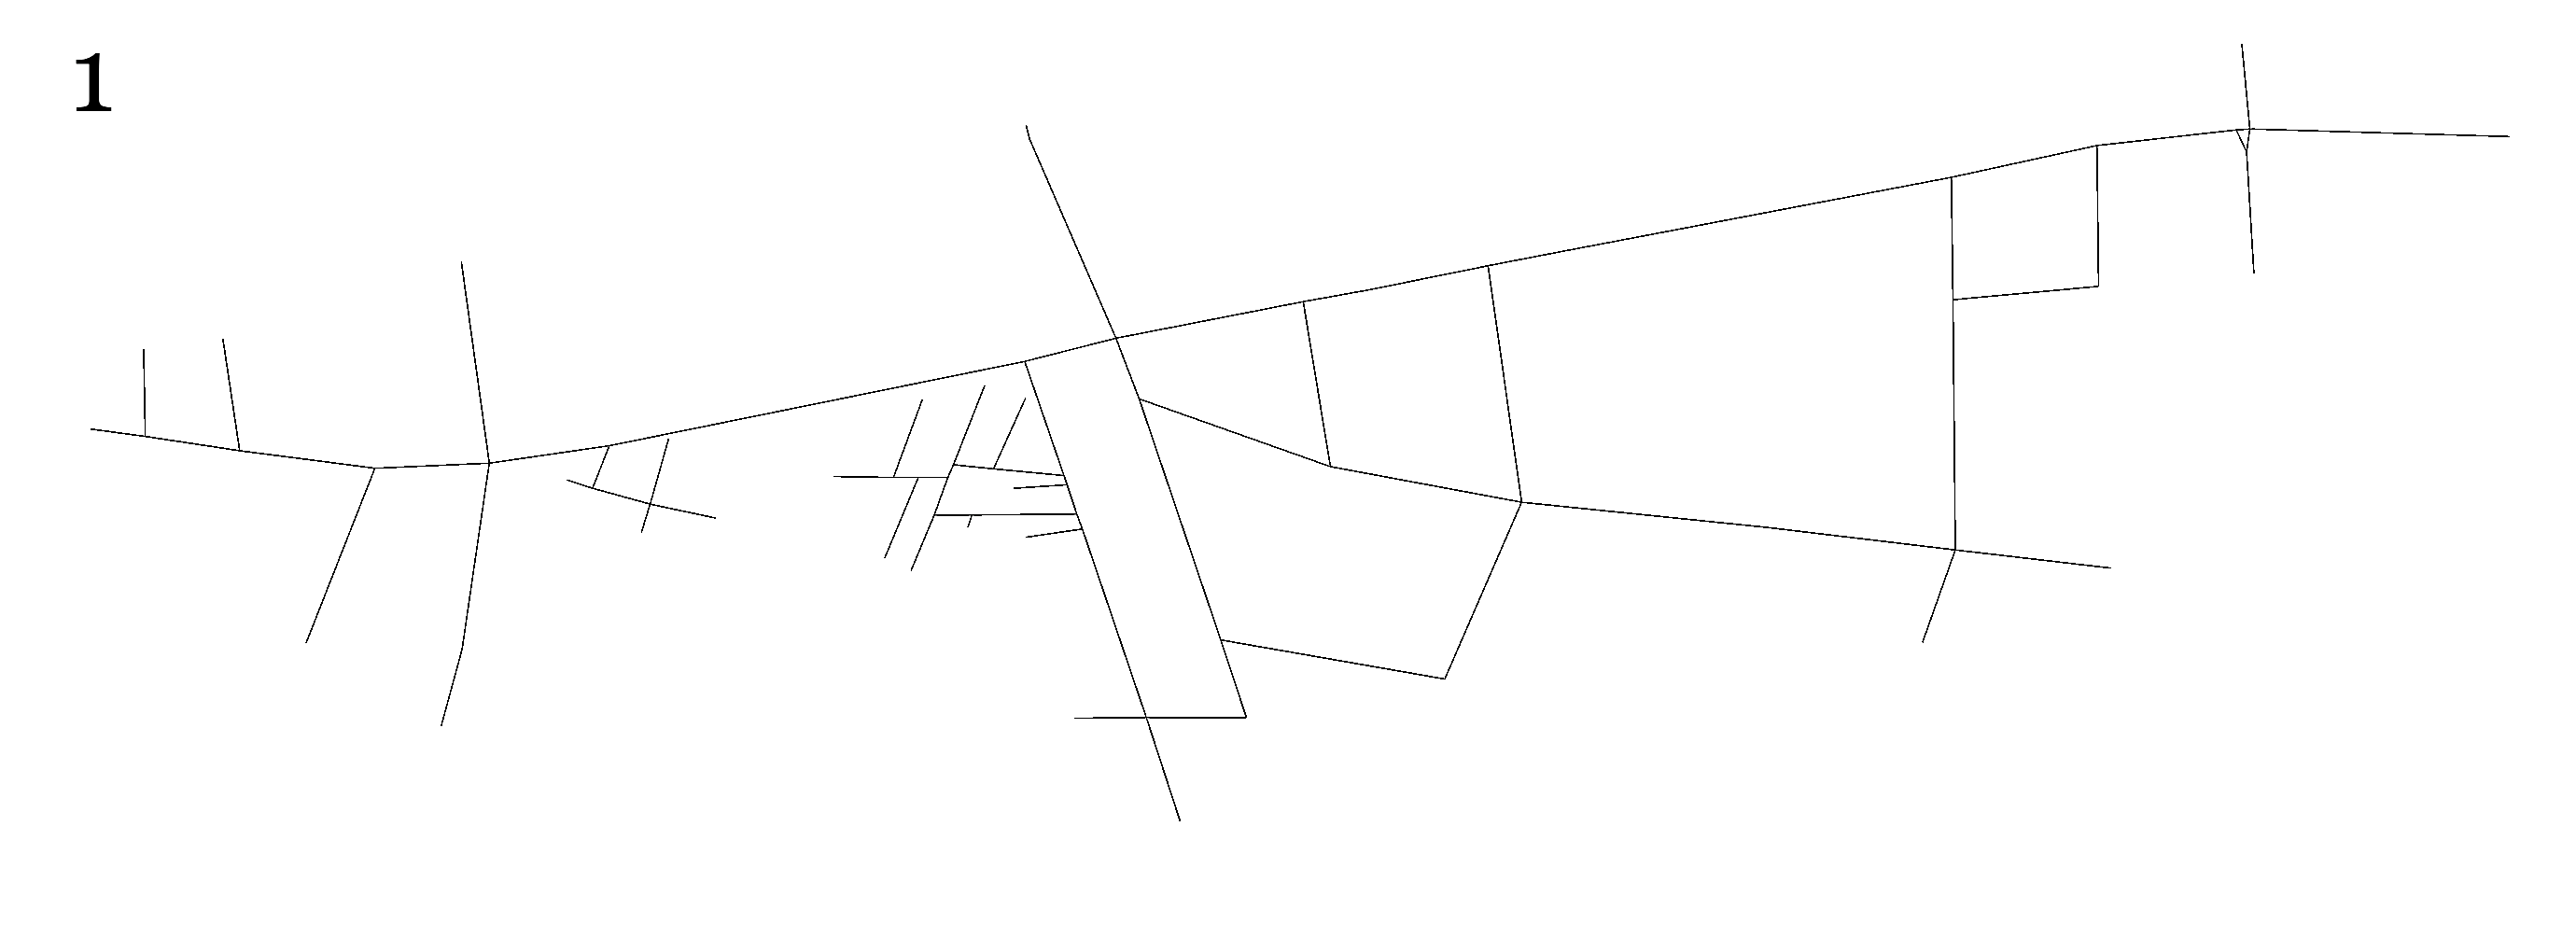
\includegraphics[width=.5\textwidth]{Images/vis-step-one.png}
    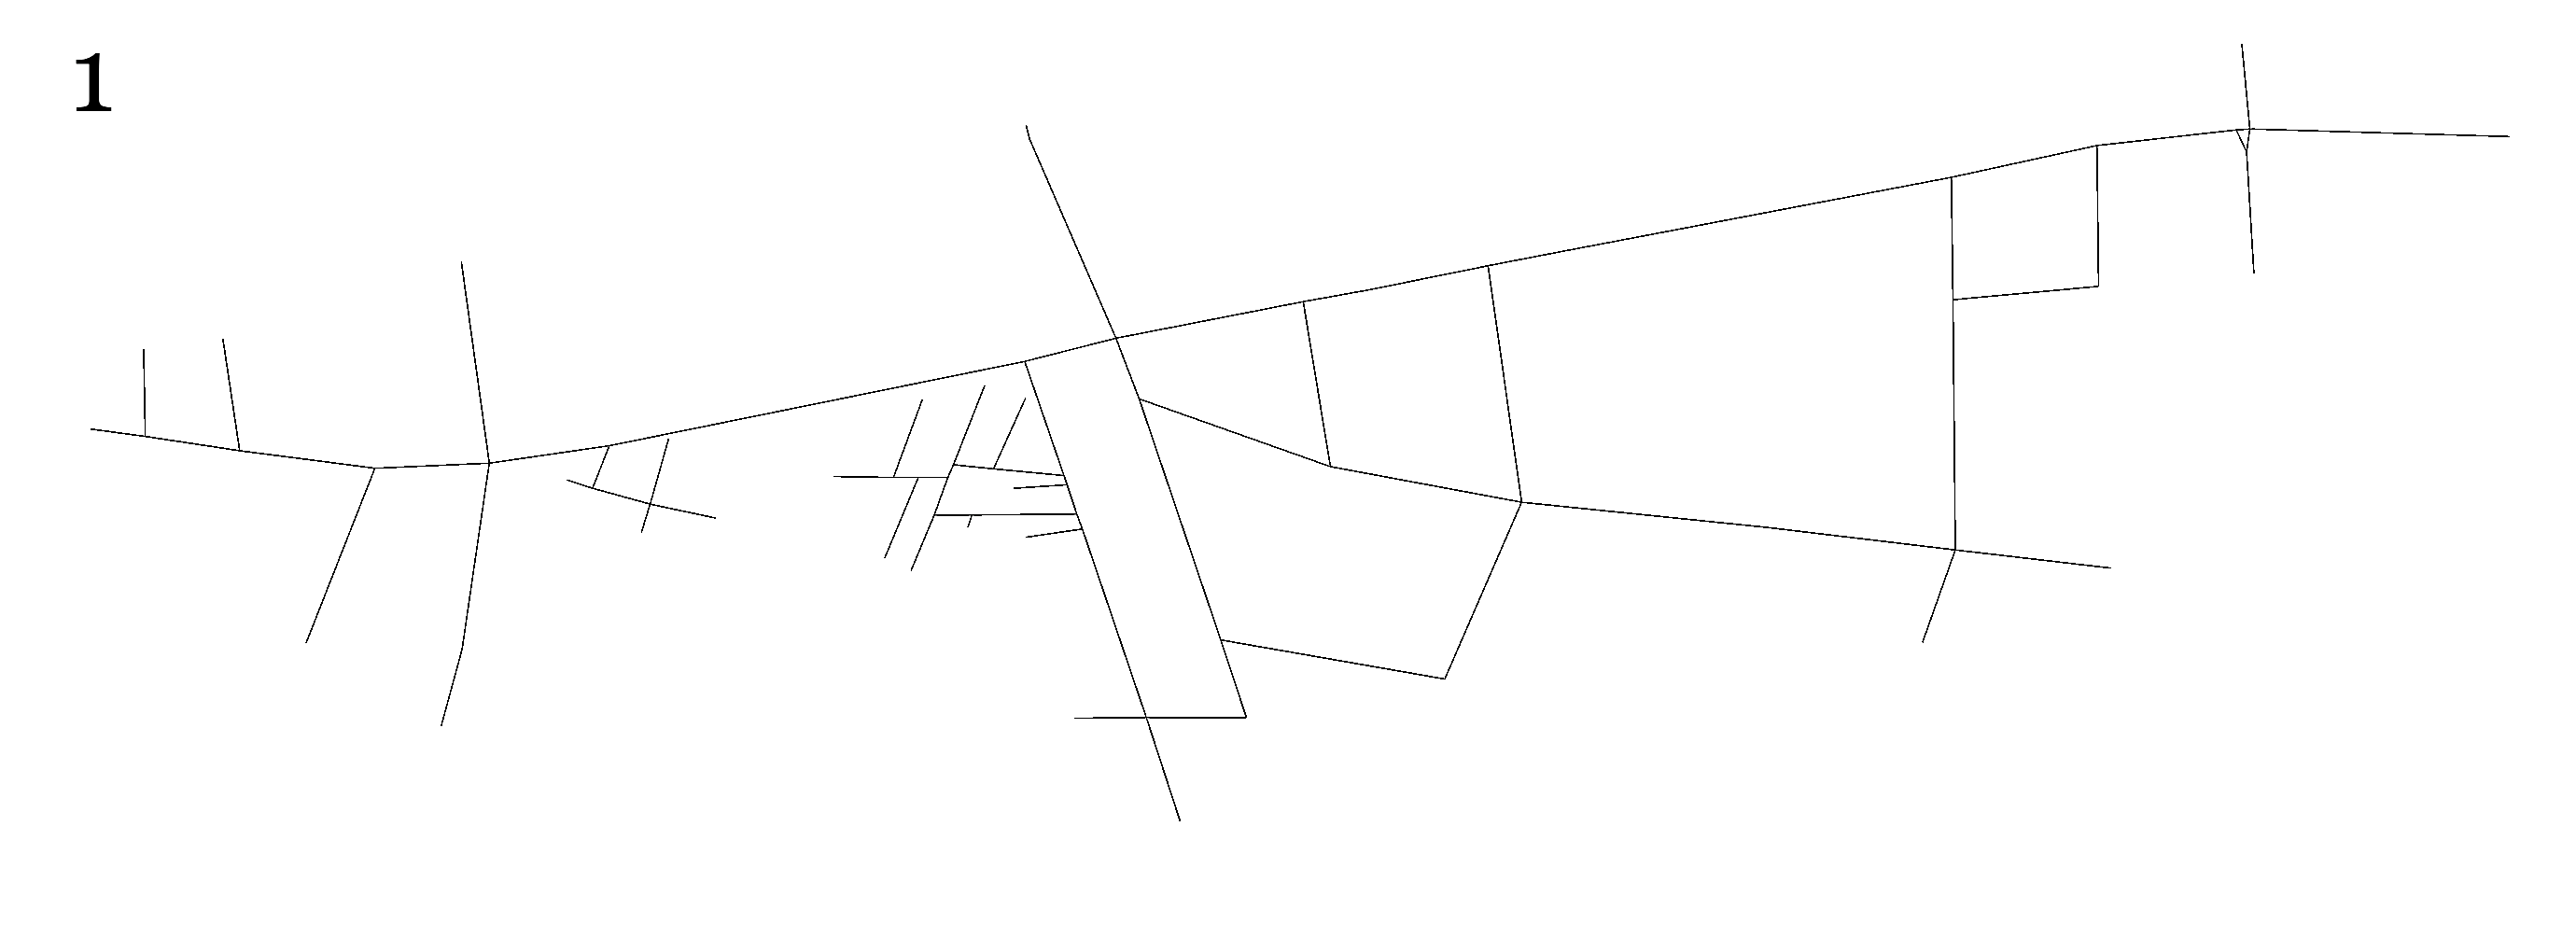
\includegraphics[width=.5\textwidth]{Images/vis-step-one.png}
\caption[]{Two consecutive steps in the visualization. Every black line represents an edge.}
\label{fig:two-steps}
\end{figure}

In \cref{fig:two-steps} we can see that we got a good basic understanding of how the framework evolves.
We added the tiles to the visualization on a similar way.
A tile is alway displayed whenever its first edge is processed.

\begin{figure}[H]
    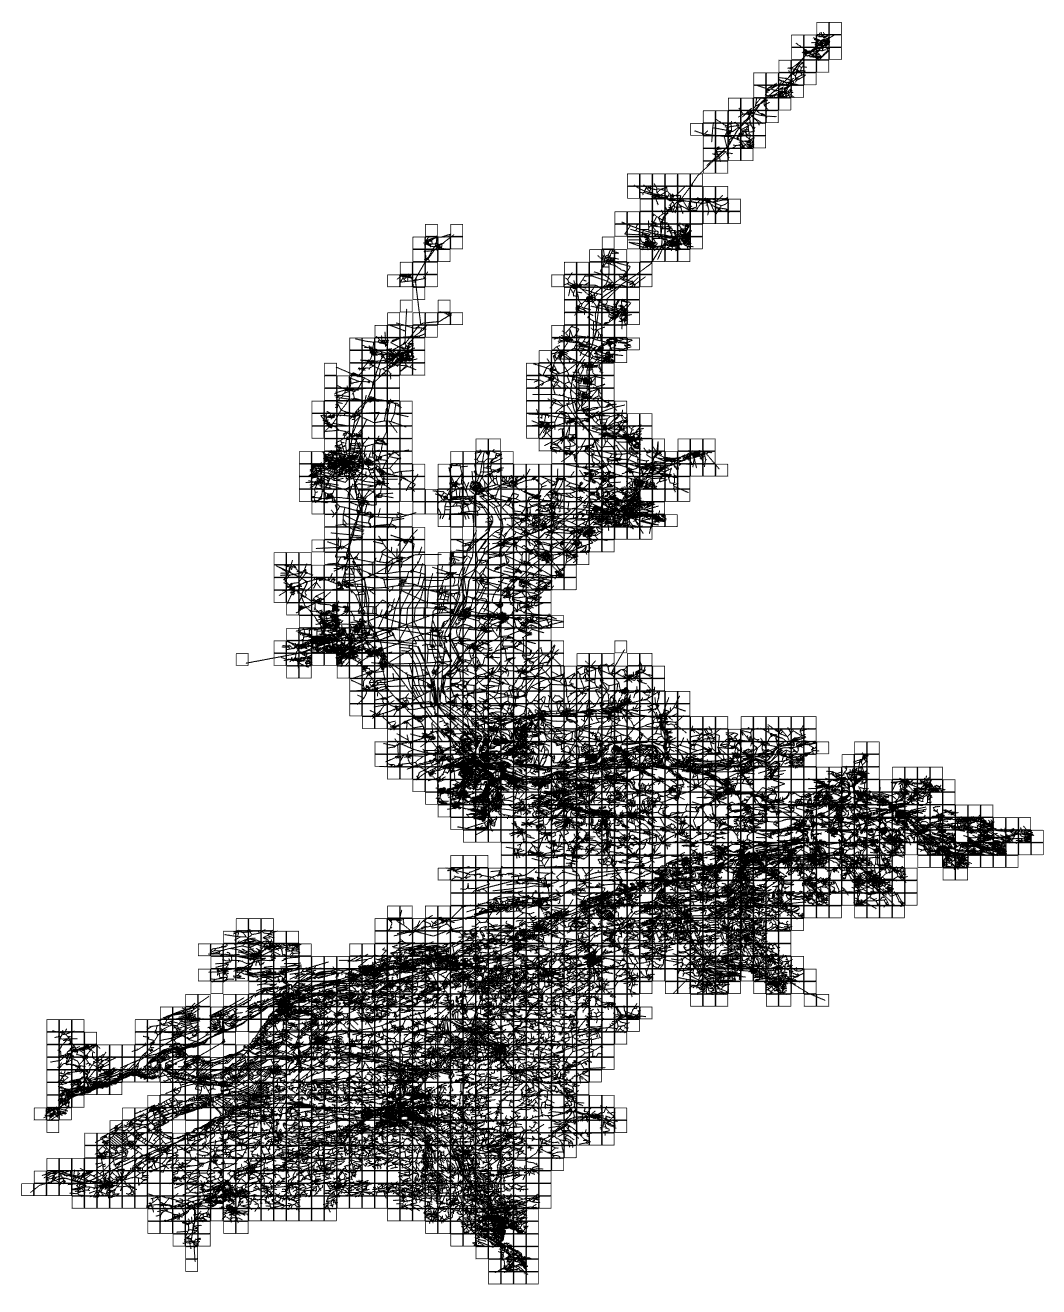
\includegraphics[width=\textwidth]{Images/vis-rectangular-tiles.png}
\caption[]{Representing tiles through rectangles.}
\label{fig:rectangle_tiles}
\end{figure}

The strategy of displaying edges and tiles as seen in  \cref{fig:rectangle_tiles} has worked great on smaller routes and it was possible to track the state of the framework quite good.

\begin{figure}[H]
    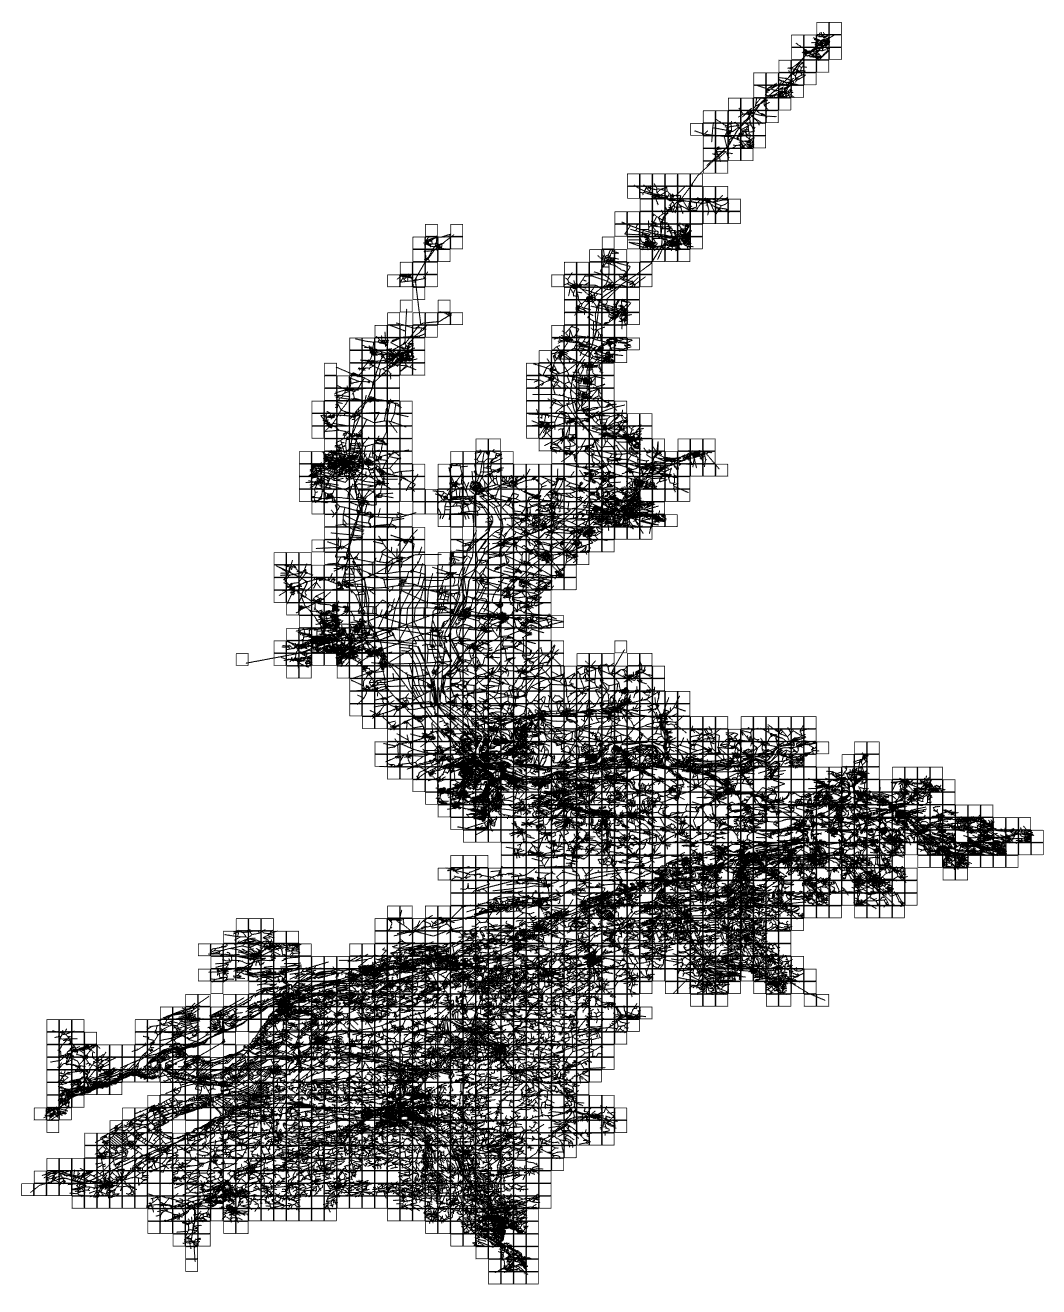
\includegraphics[width=\textwidth]{Images/vis-rectangular-tiles.png}
\caption[]{Representing tiles through rectangles on a bigger route.}
\label{fig:rectangle_tiles_big}
\end{figure}

On bigger routes, this visualization lacks in comprehensibility as we can see in \cref{fig:rectangle_tiles_big}.
In addition, we experienced performance issues due to the amount of displayed elements and one step was hard to distinguish from its predecessor.
Therefore we removed the edges from our visualization.

\begin{figure}[H]
        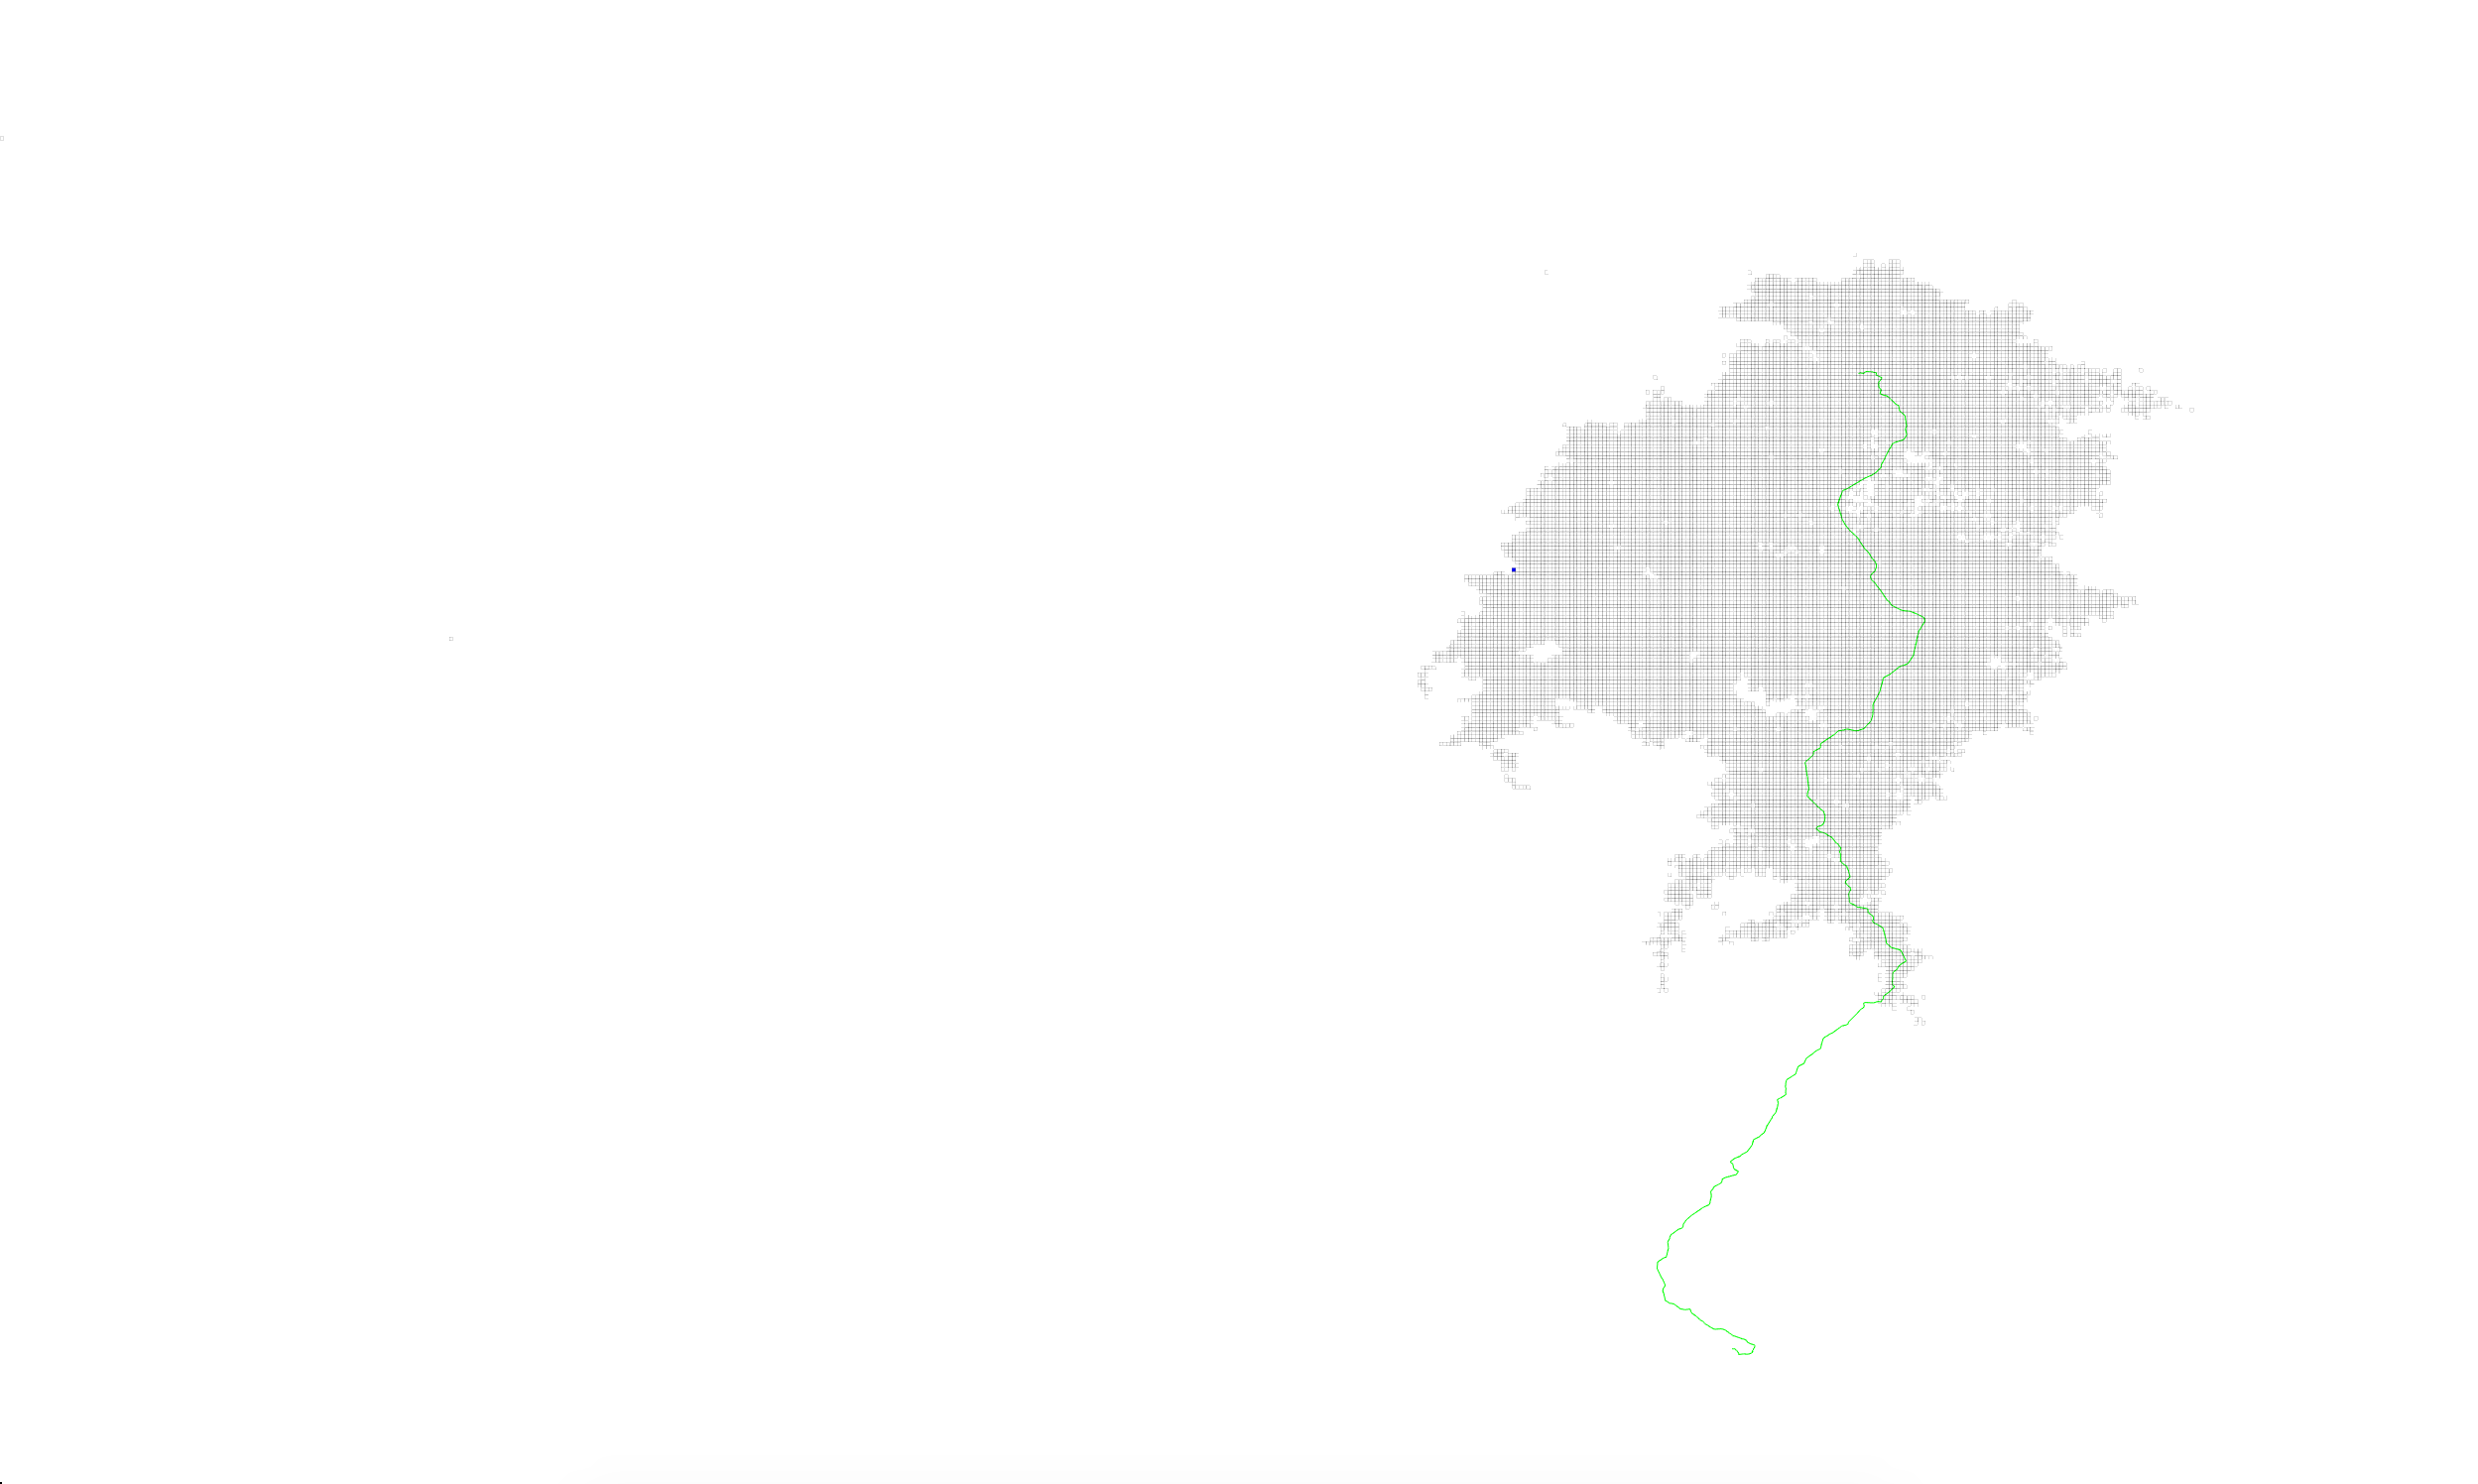
\includegraphics[width=\textwidth]{Images/vis-current-tile.png}
\caption[]{Representing tiles only through rectangles.}
\label{fig:only_rectangles}
\end{figure}

In \cref{fig:only_rectangles} we see an uncluttered representation based on tiles.
By removing the edges we also experienced a tremendous performance boost.


\paragraph{Outlining the current step}

In the tile-based visualization, we can see in \cref{fig:only_rectangles} it is hard to see whenever a tile is added to the graph.
Furthermore, we had no chance to notice which tile the framework is currently processing.
Therefore a first approach was to color the tile in which edges are currently processed.
For adding an understanding about which route the framework is supposed to find and the possibility to see how far the framework already proceeded to find the path, we added the resulting path of the framework to the visualization

\begin{figure}[H]
        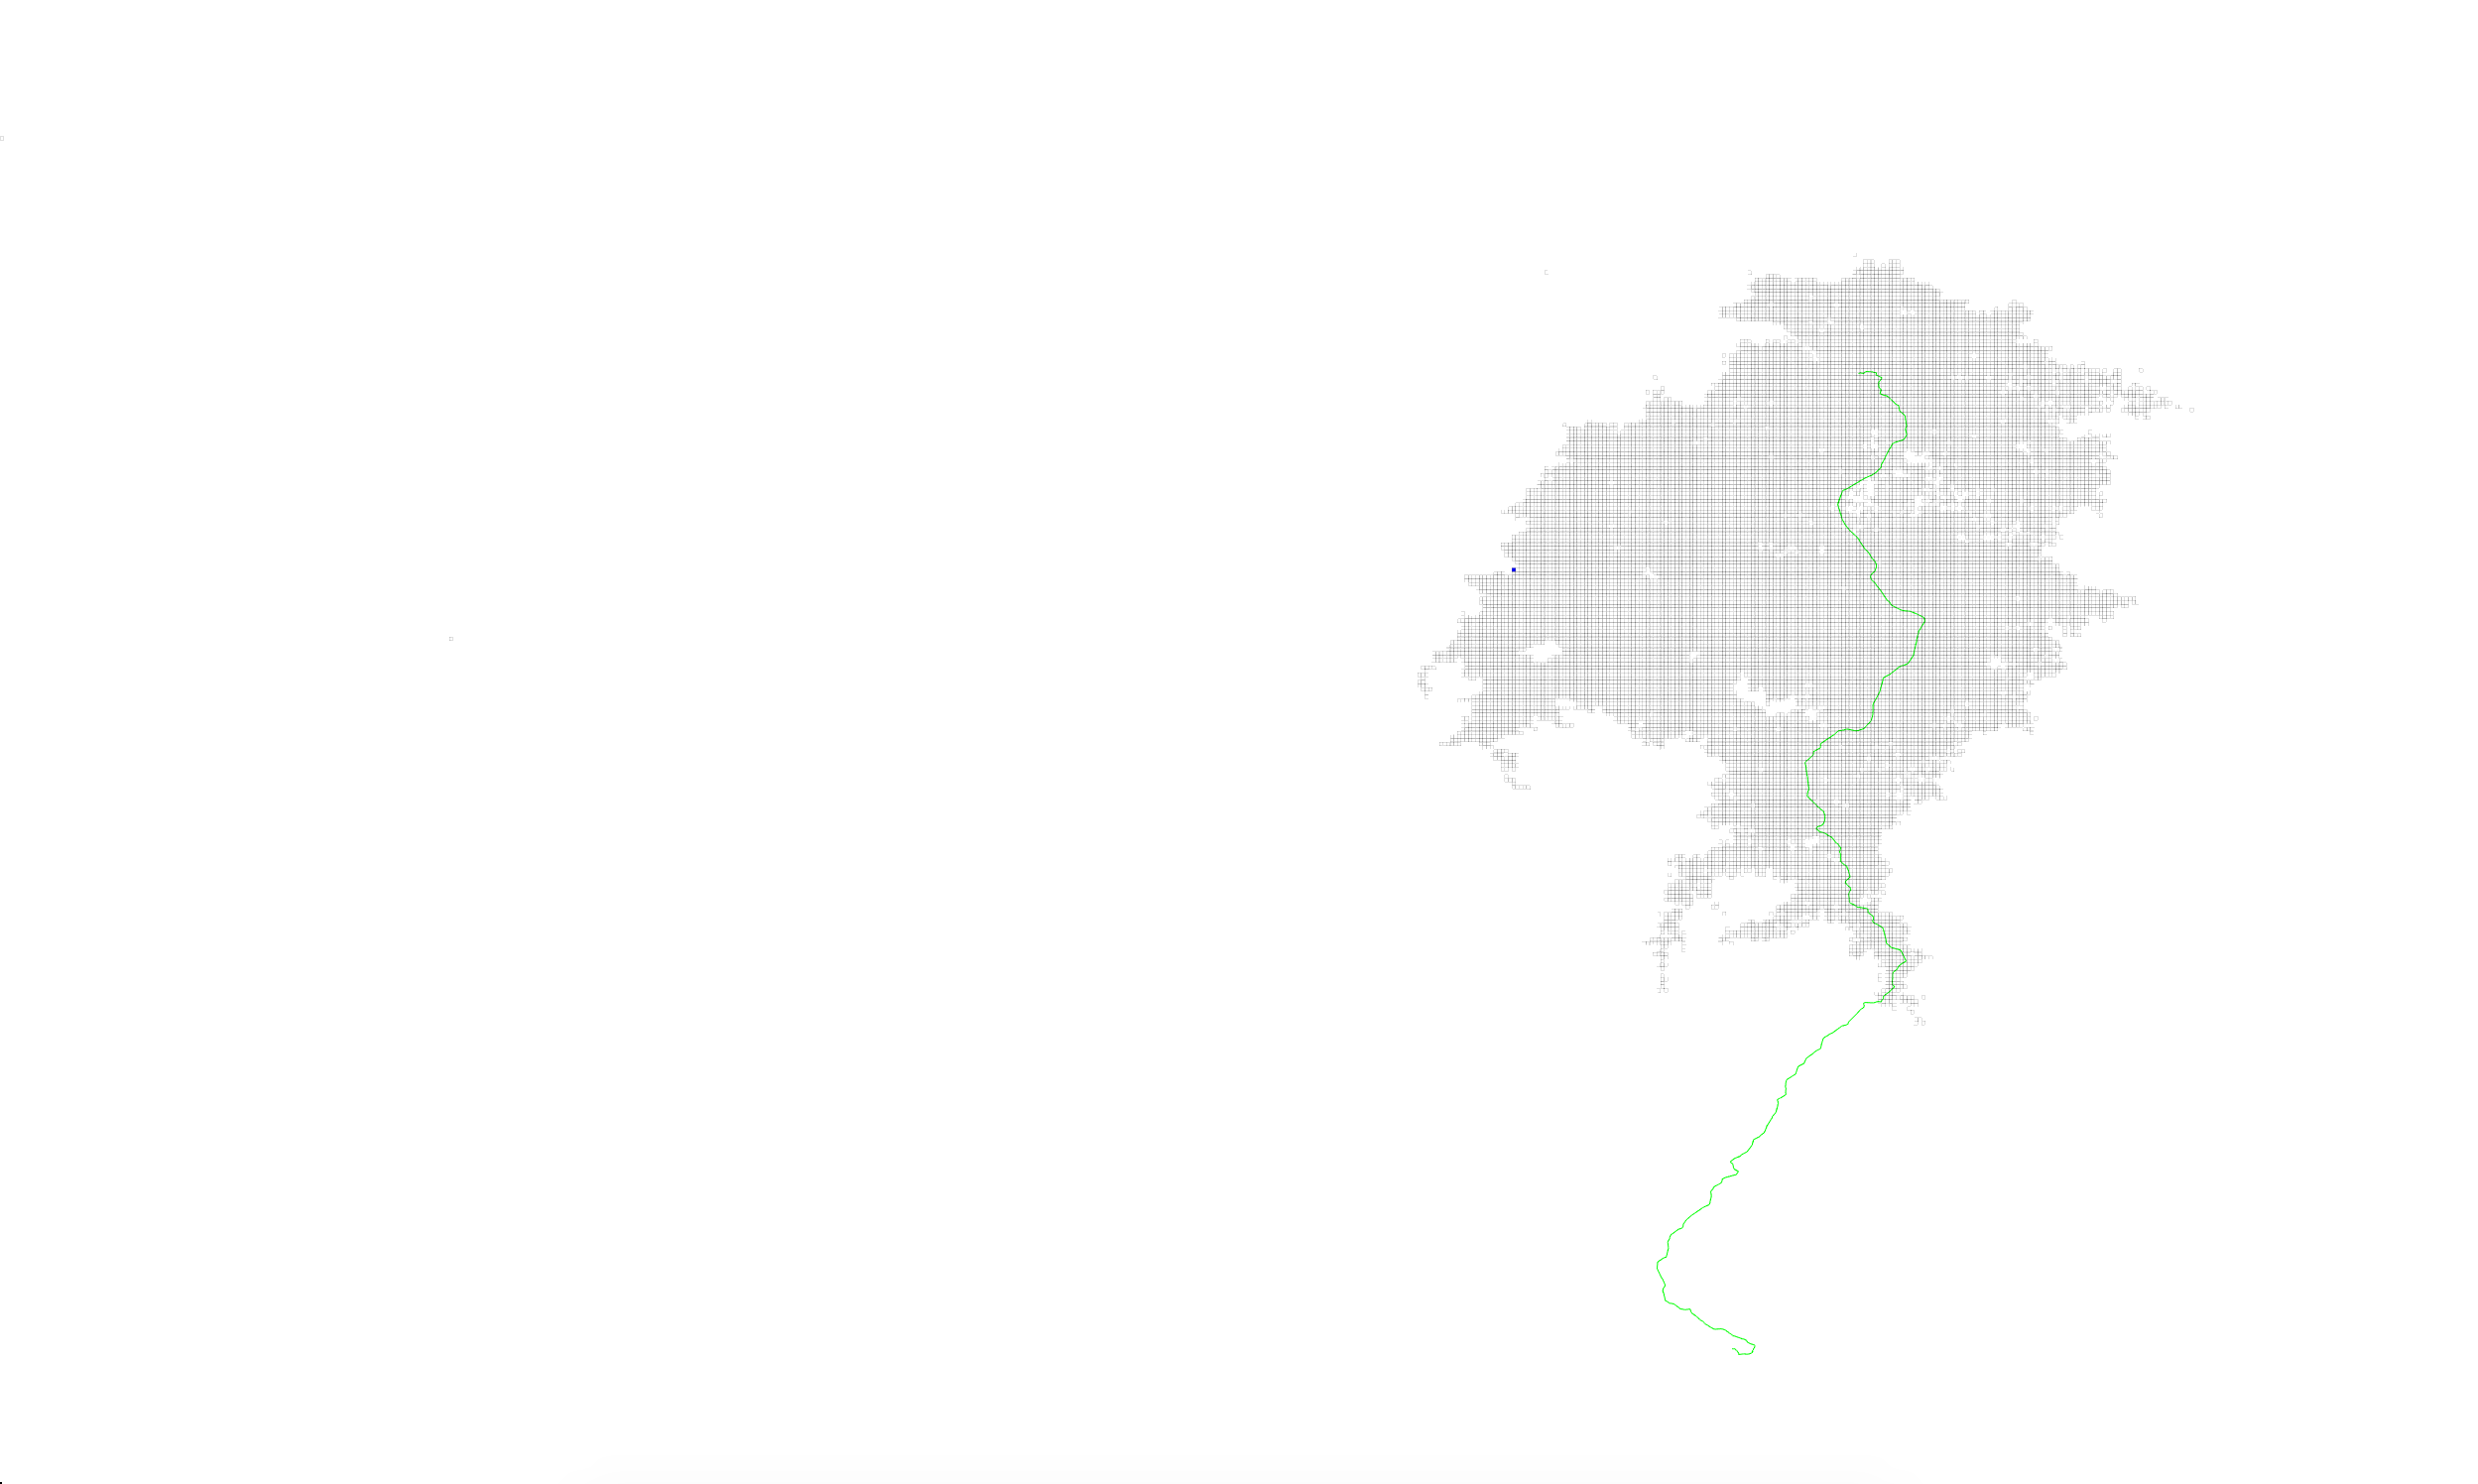
\includegraphics[width=\textwidth]{Images/vis-current-tile.png}
\caption[]{Coloring the tile that is processed blue.}
\label{fig:color_current_tile}
\end{figure}

Even though this method enables us to see which tile is processed in a single image, as we can see in \cref{fig:color_current_tile}, this information was not accessible in multiple fastly successive images.
As what our visualization does, is to show multiple fastly successive images of successive states of the framework
That is wy we had to figure out a more compatible method of showing what is going on.

Hence, we developed a method, we called aging of tiles.
This method builds on the previously introduced method, but instead of uncoloring the tile immediately, it uncolors it over time.
Therefore the tile becomes a bit brighter every step of the framework.

\begin{figure}[H]
    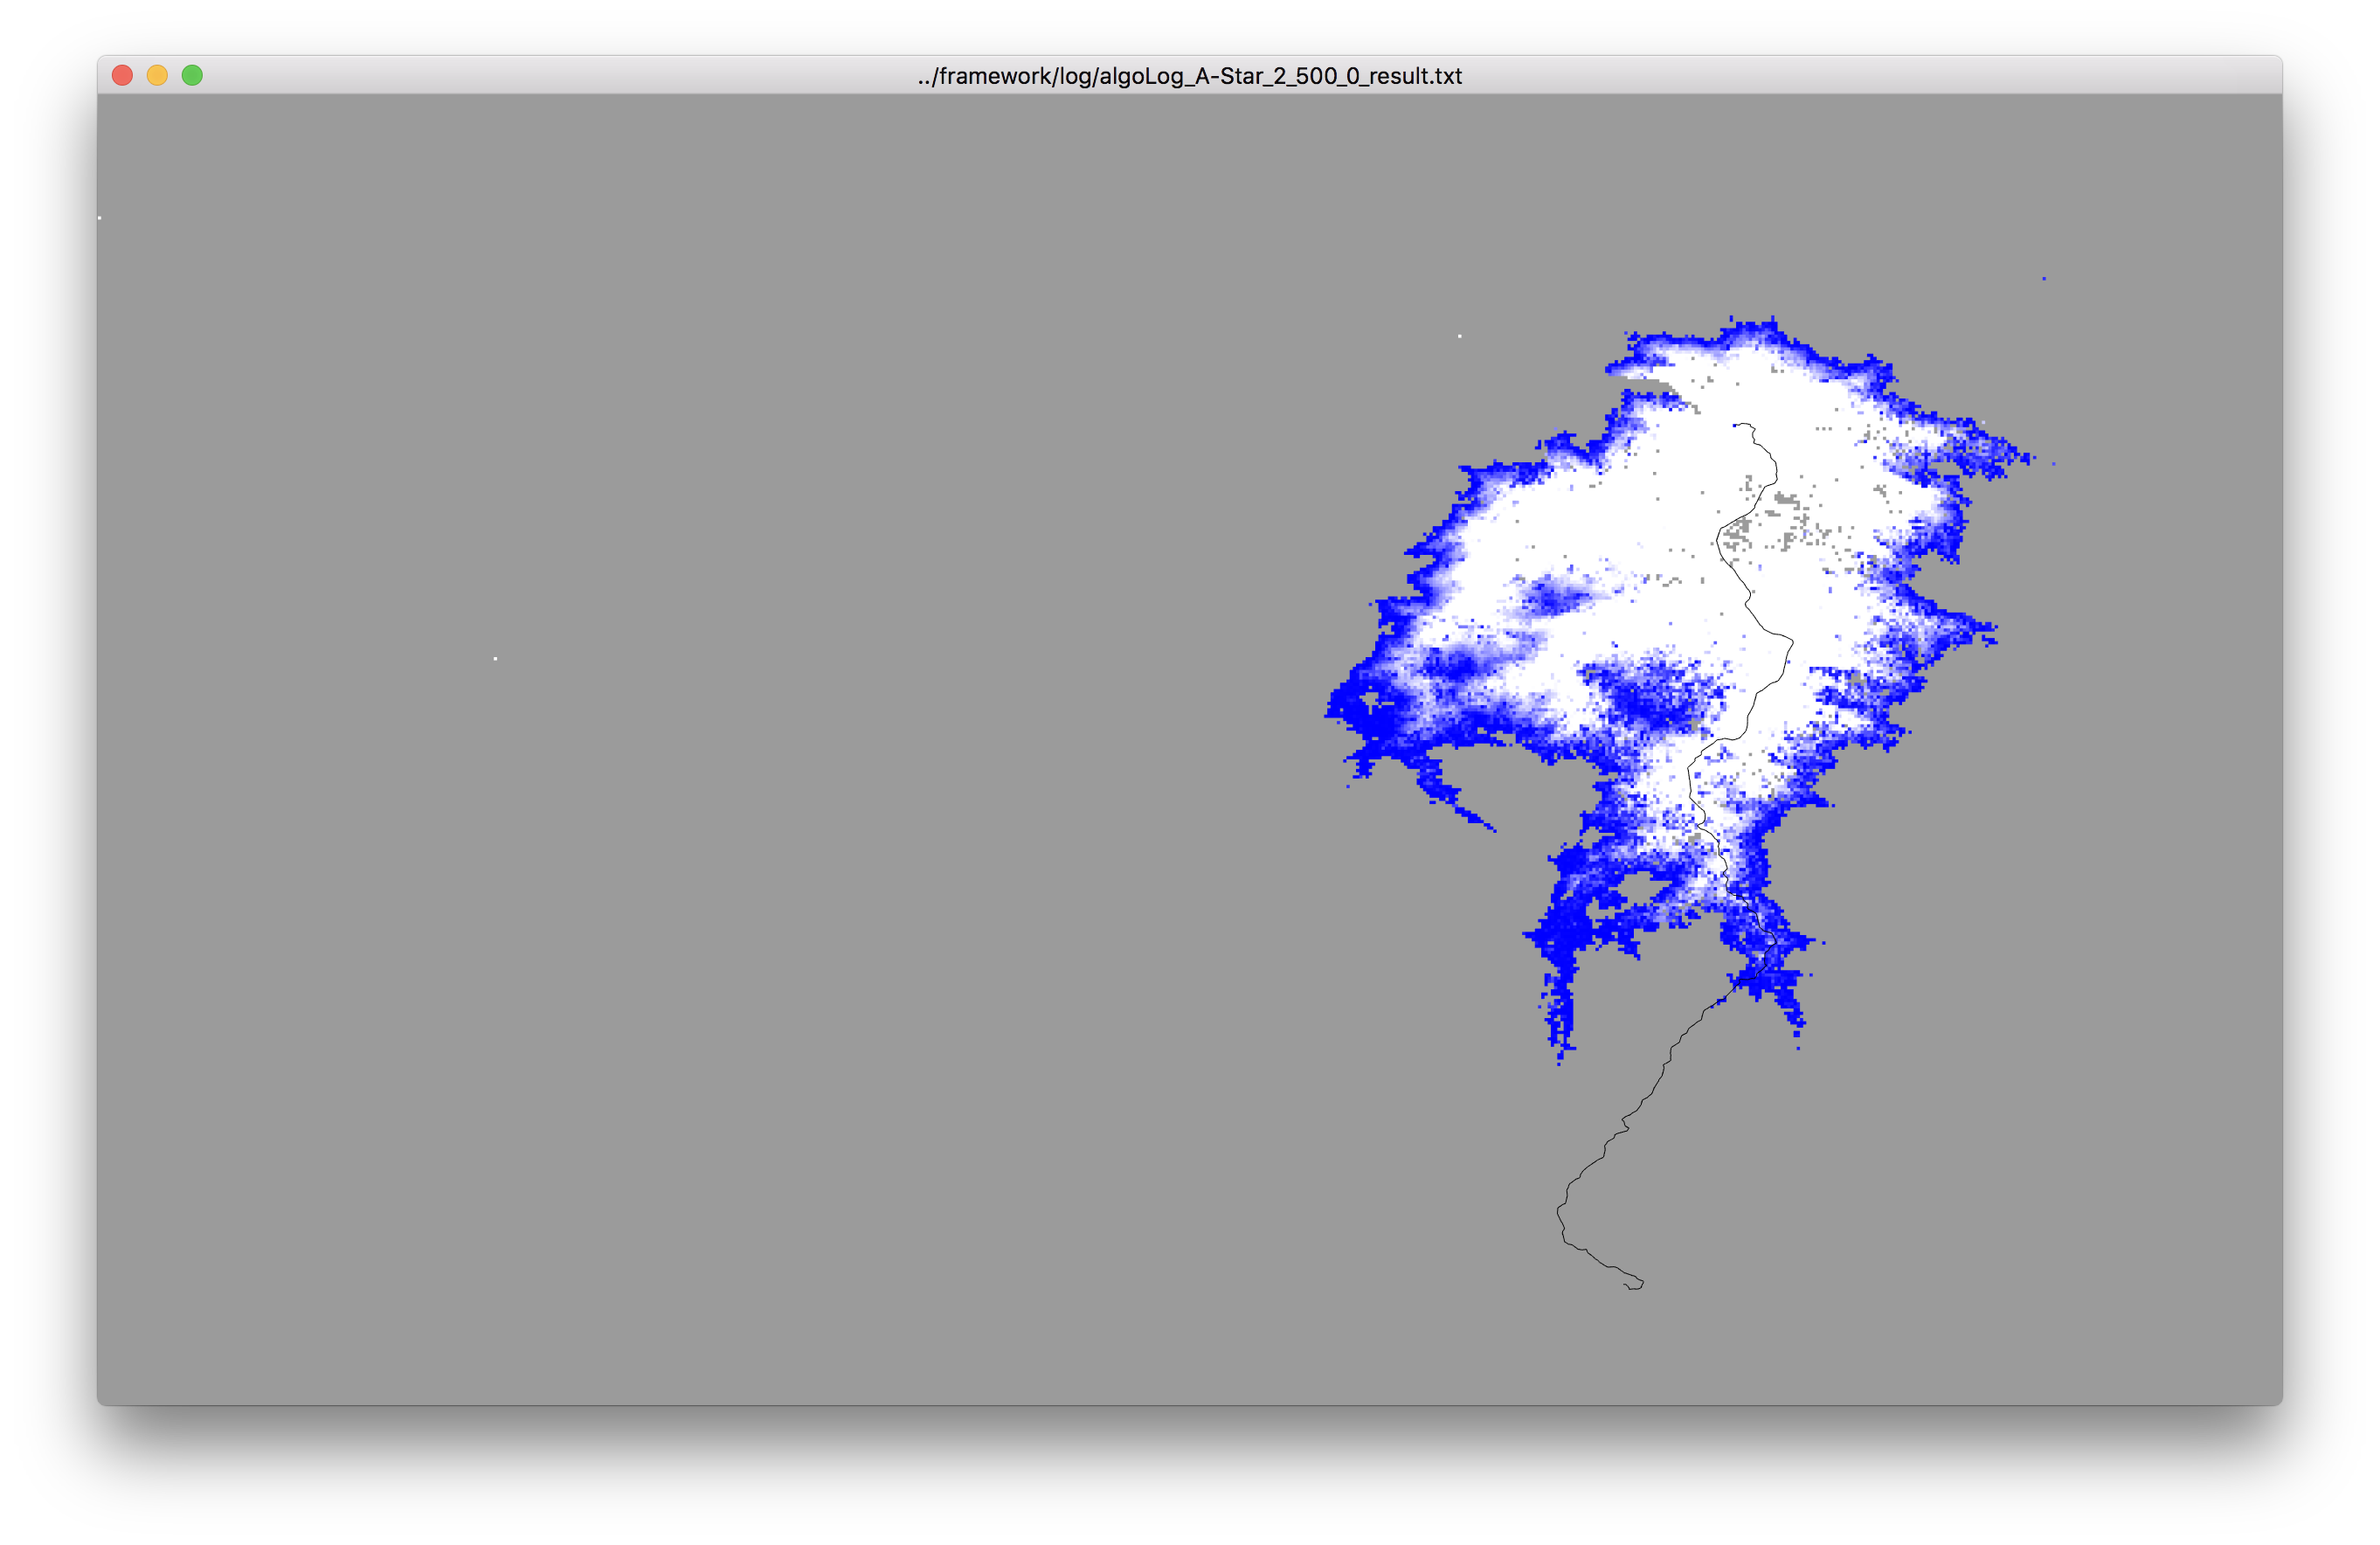
\includegraphics[width=\textwidth]{Images/vis-aged-coloring.png}
\caption[]{Age based coloring. Newly loaded tiles are colored blue and get brighter the longer they have not been loaded.}
\label{fig:color_aged_tile}
\end{figure}

In \cref{fig:color_aged_tile} we see that this approach leads to a much better understanding of the sequence of tile-loads.
Thereby it adds a lot of comprehensibility on how the algorithm performs on the underlying graph.
In the specific case displayed in \cref{fig:color_aged_tile} for example, we can see that most of the recently loaded tiles are located on the outside of the explored graph, but there are three bigger parts in the inner part which should maybe be examined more specific.

\paragraph{Showing the right section of the graph}
In this paragraph, we are going to explain something we took for granted previously in this chapter, but needed to figure out as well.
Somehow, we have to decide where we want to place the elements in the visualization.
We want to show the same element at exactly the same spot in the whole visualization.
Therefore the visualization needs to consider which section of the graph it wants to show before it displays the first element.
As the displayed graph grows as the algorithm progresses there is the risk of growing out of the screen when we estimate the final graph too small.
On the other side, a graph that is estimated to big, which would result in much unused space on out screen.

We considered multiple approaches to solve this issue.
Firstly we developed an estimation method, that estimates the extent of the explored graph of the fully evolved algorithm.
For estimating, this method uses the linear distance between start and target node as the basis.
Because we need to make that the visualization shows everything that is going to happen during the framework, it uses a little more than the distance between start and target node as the radius of a circle around the start node.
This circle then flushs with the borders of the visualization, as we assume that the final graph is going to fill this circle.

\begin{figure}[H]
    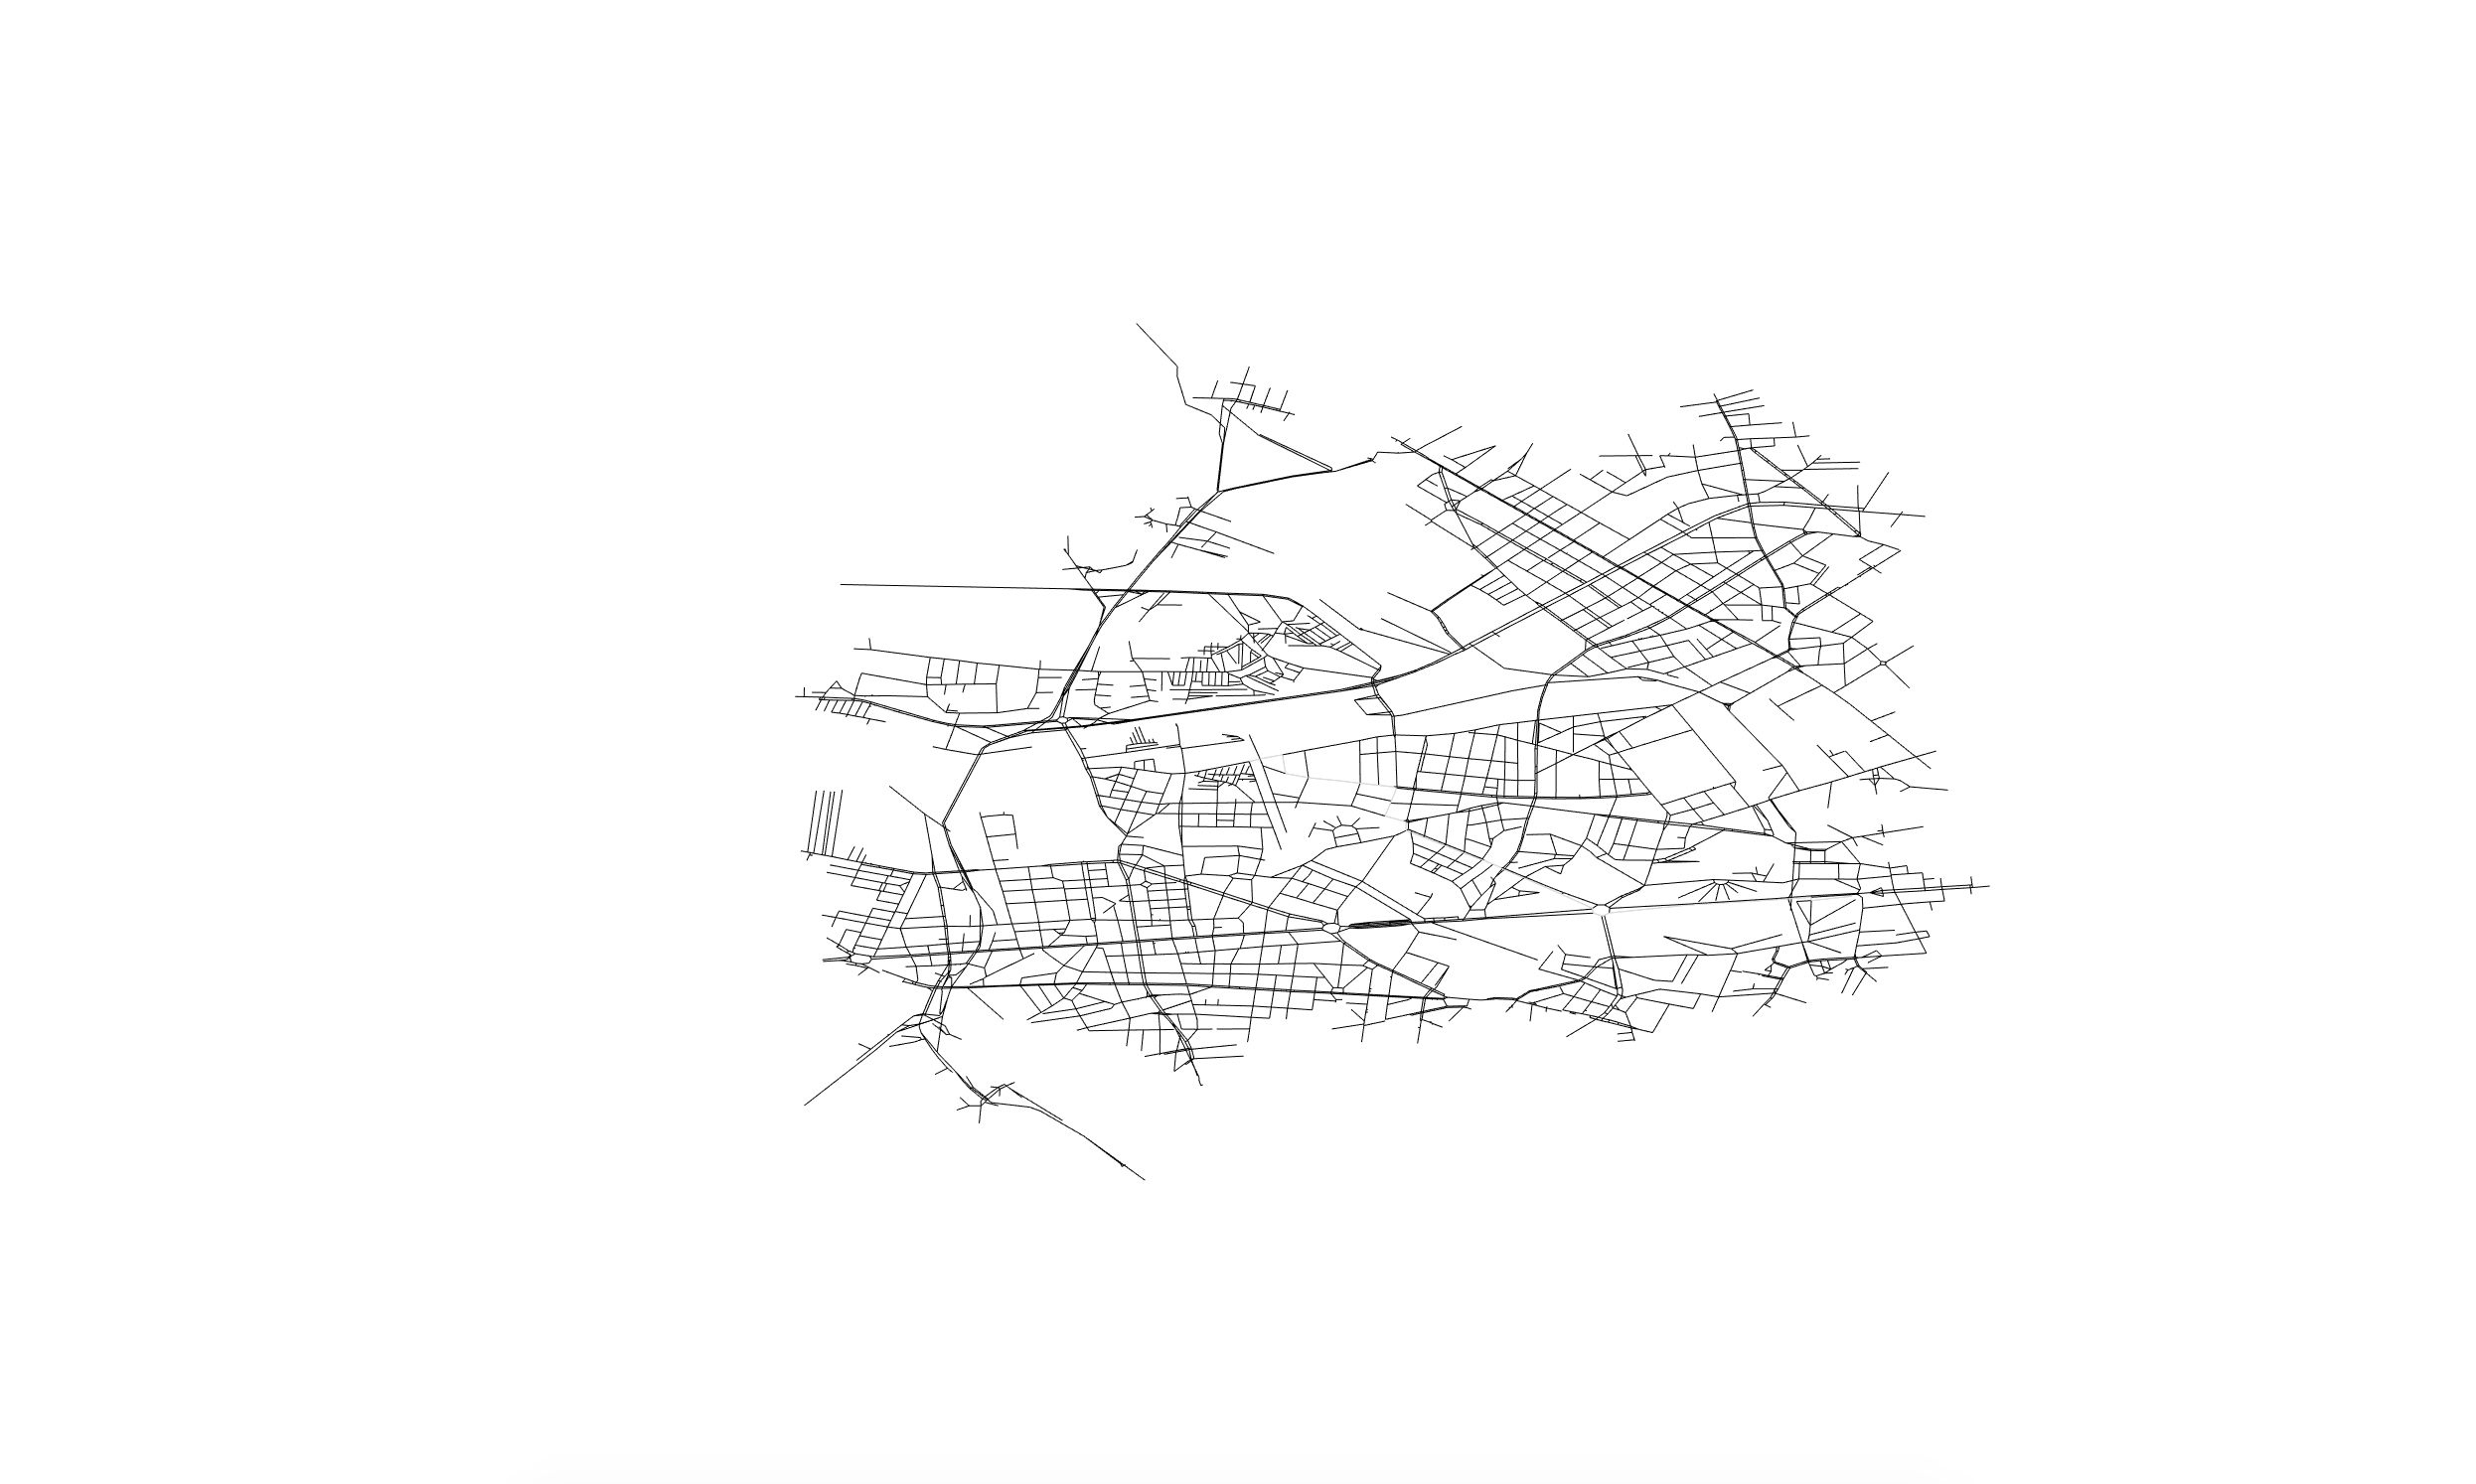
\includegraphics[width=\textwidth]{Images/vis-estimation.png}
\caption[]{Estimation method}
\label{fig:estimation}
\end{figure}

In \cref{fig:estimation} we can see that we have got quite a lot unused space using this estimation.
Even though this estimation is quite generous, the actual graph could still grow over this circle.
In general, it is, of course, possible to provide better estimations, but the more precise we would like the estimation to be, the more information we would need about the specific algorithm and the underlying graph, which we want to avoid.

Another method would be to iterate over the specific framework before visualizing it, and therefore find the exact borders of the graph.
With this knowledge, we could then adjust the shown section to exactly fit the fully evolved graph.

\begin{figure}[H]
    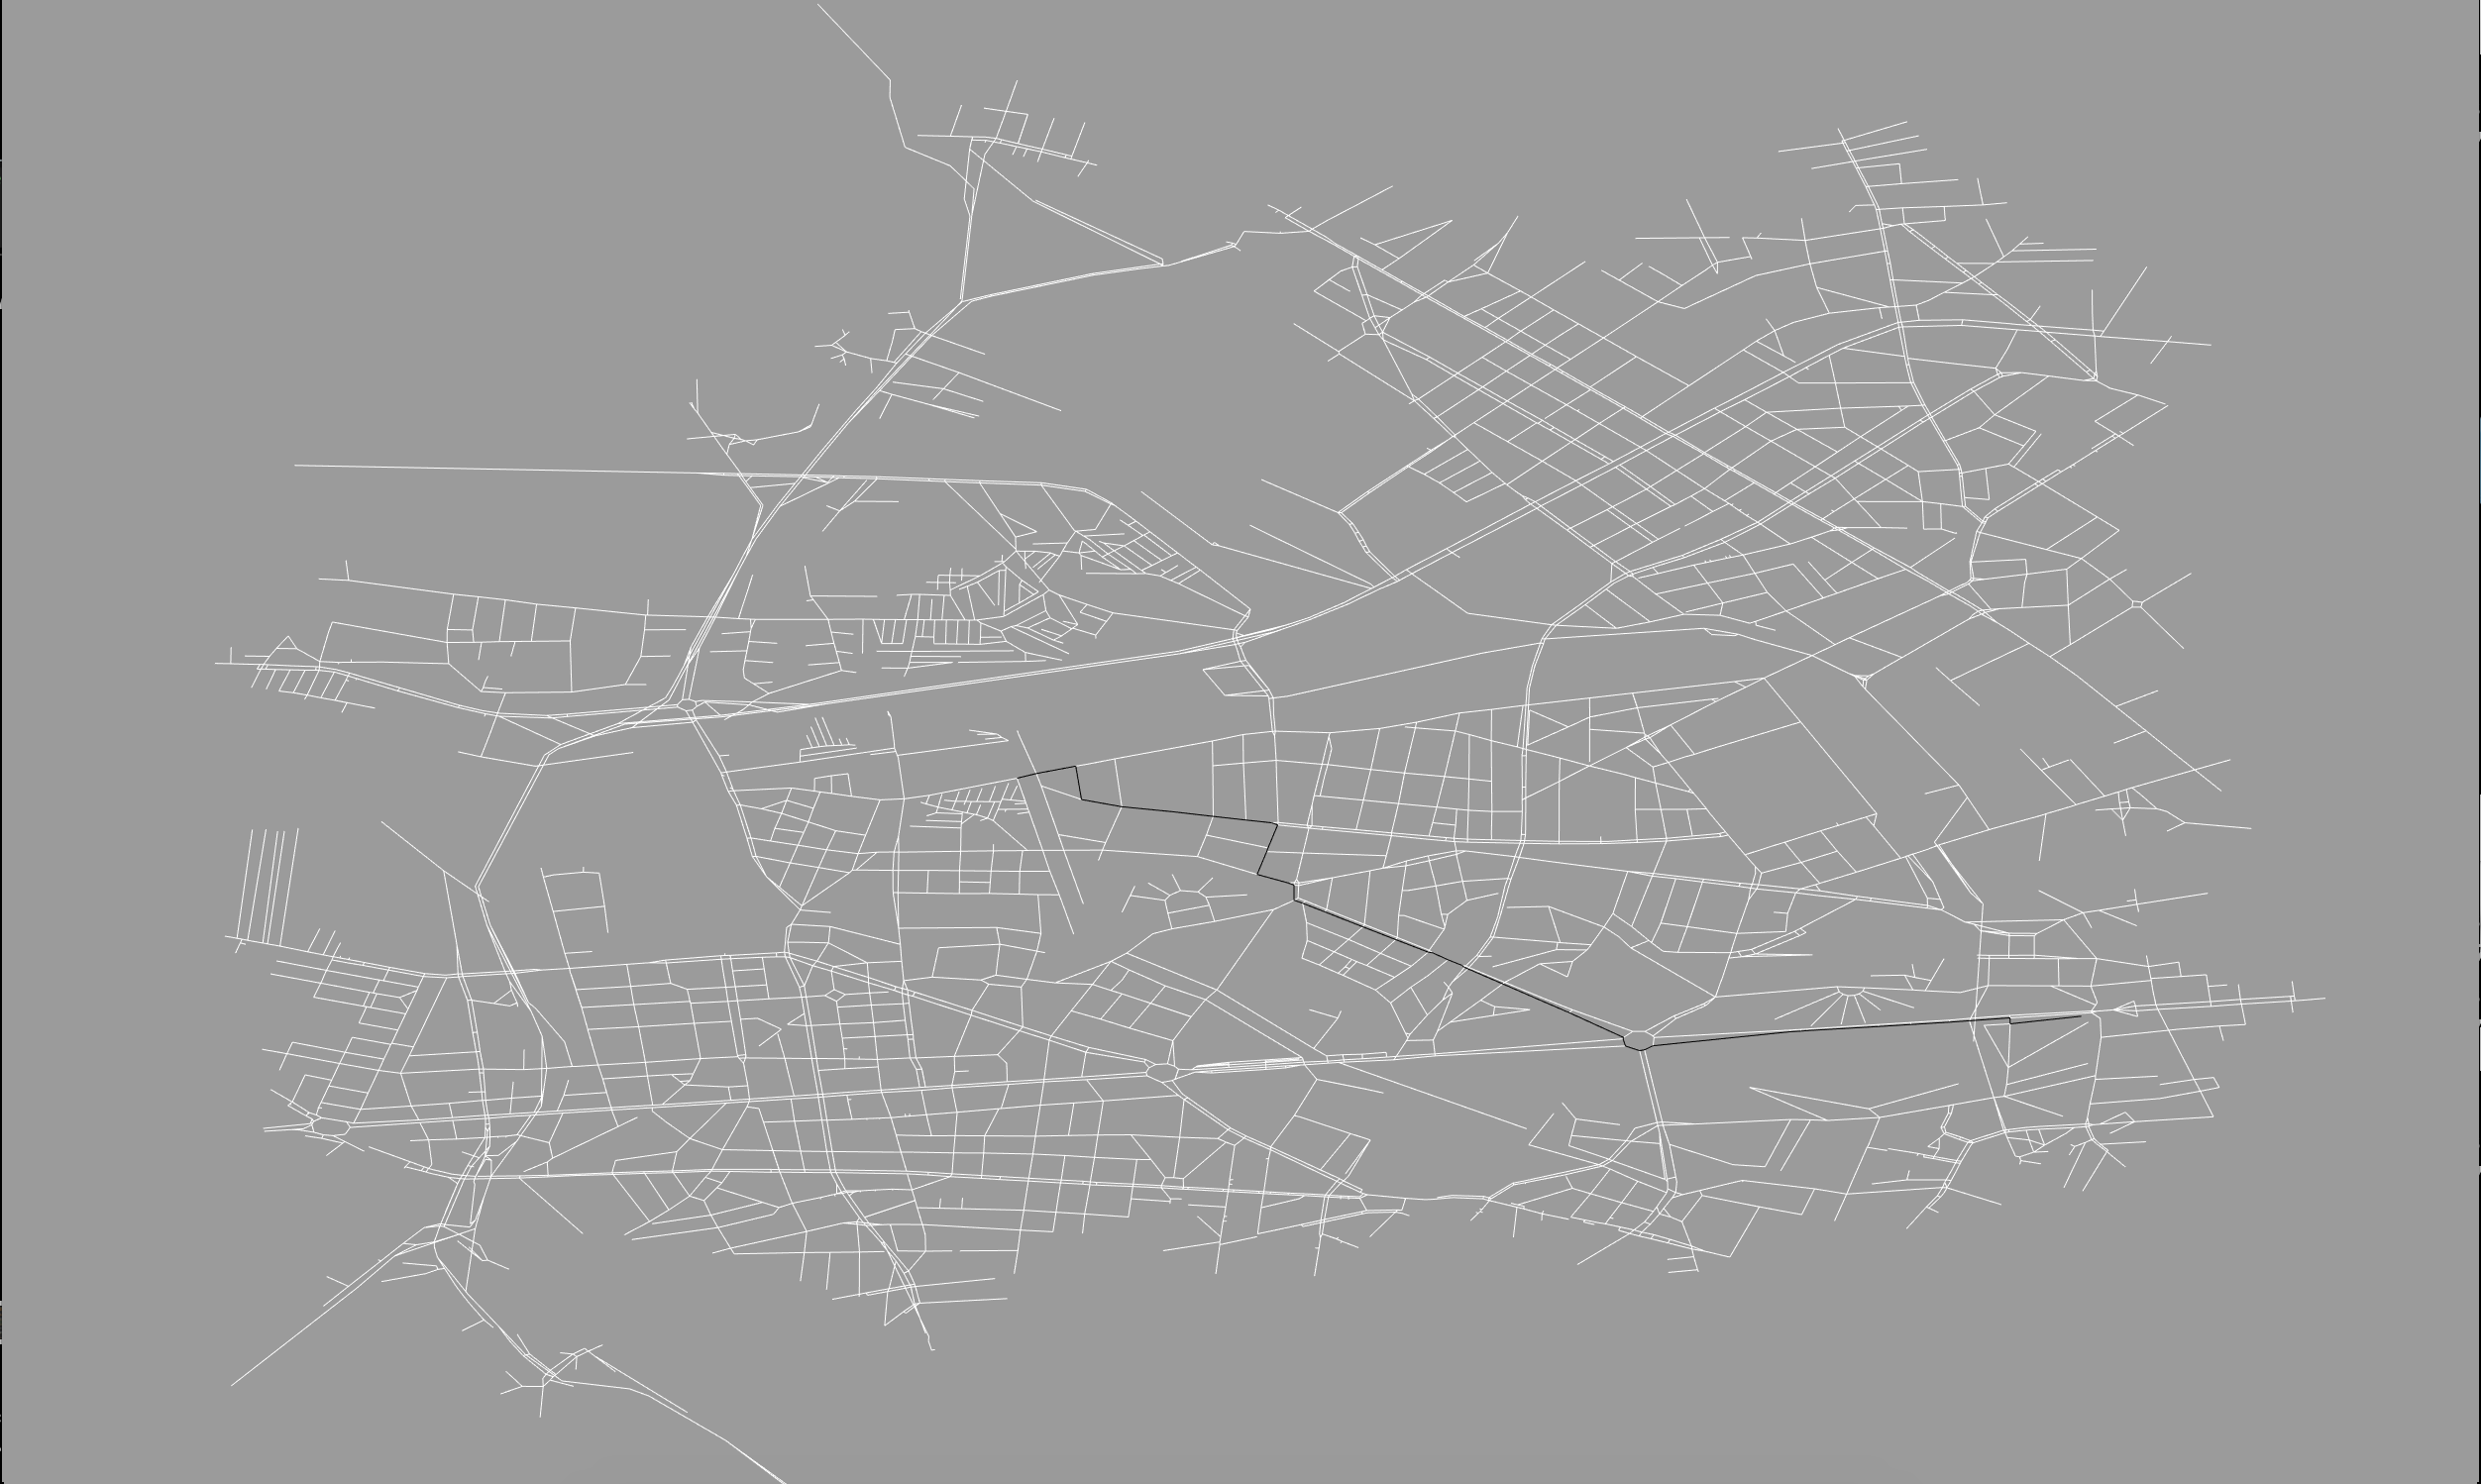
\includegraphics[width=\textwidth]{Images/vis-preprocessing.png}
\caption[]{Preprocessing method}
\label{fig:preprocessing}
\end{figure}

\cref{fig:preprocessing} shows a visualization that uses the entire available space on one axis.
As this method is using the same scale on both axes there could be bigger unused space on the other axis.

Based on this we developed another method, that changes the scale on one of the axes to fit the window of the visualization as well.
Thereby it spreads the graph over the whole screen.

\begin{figure}[H]
    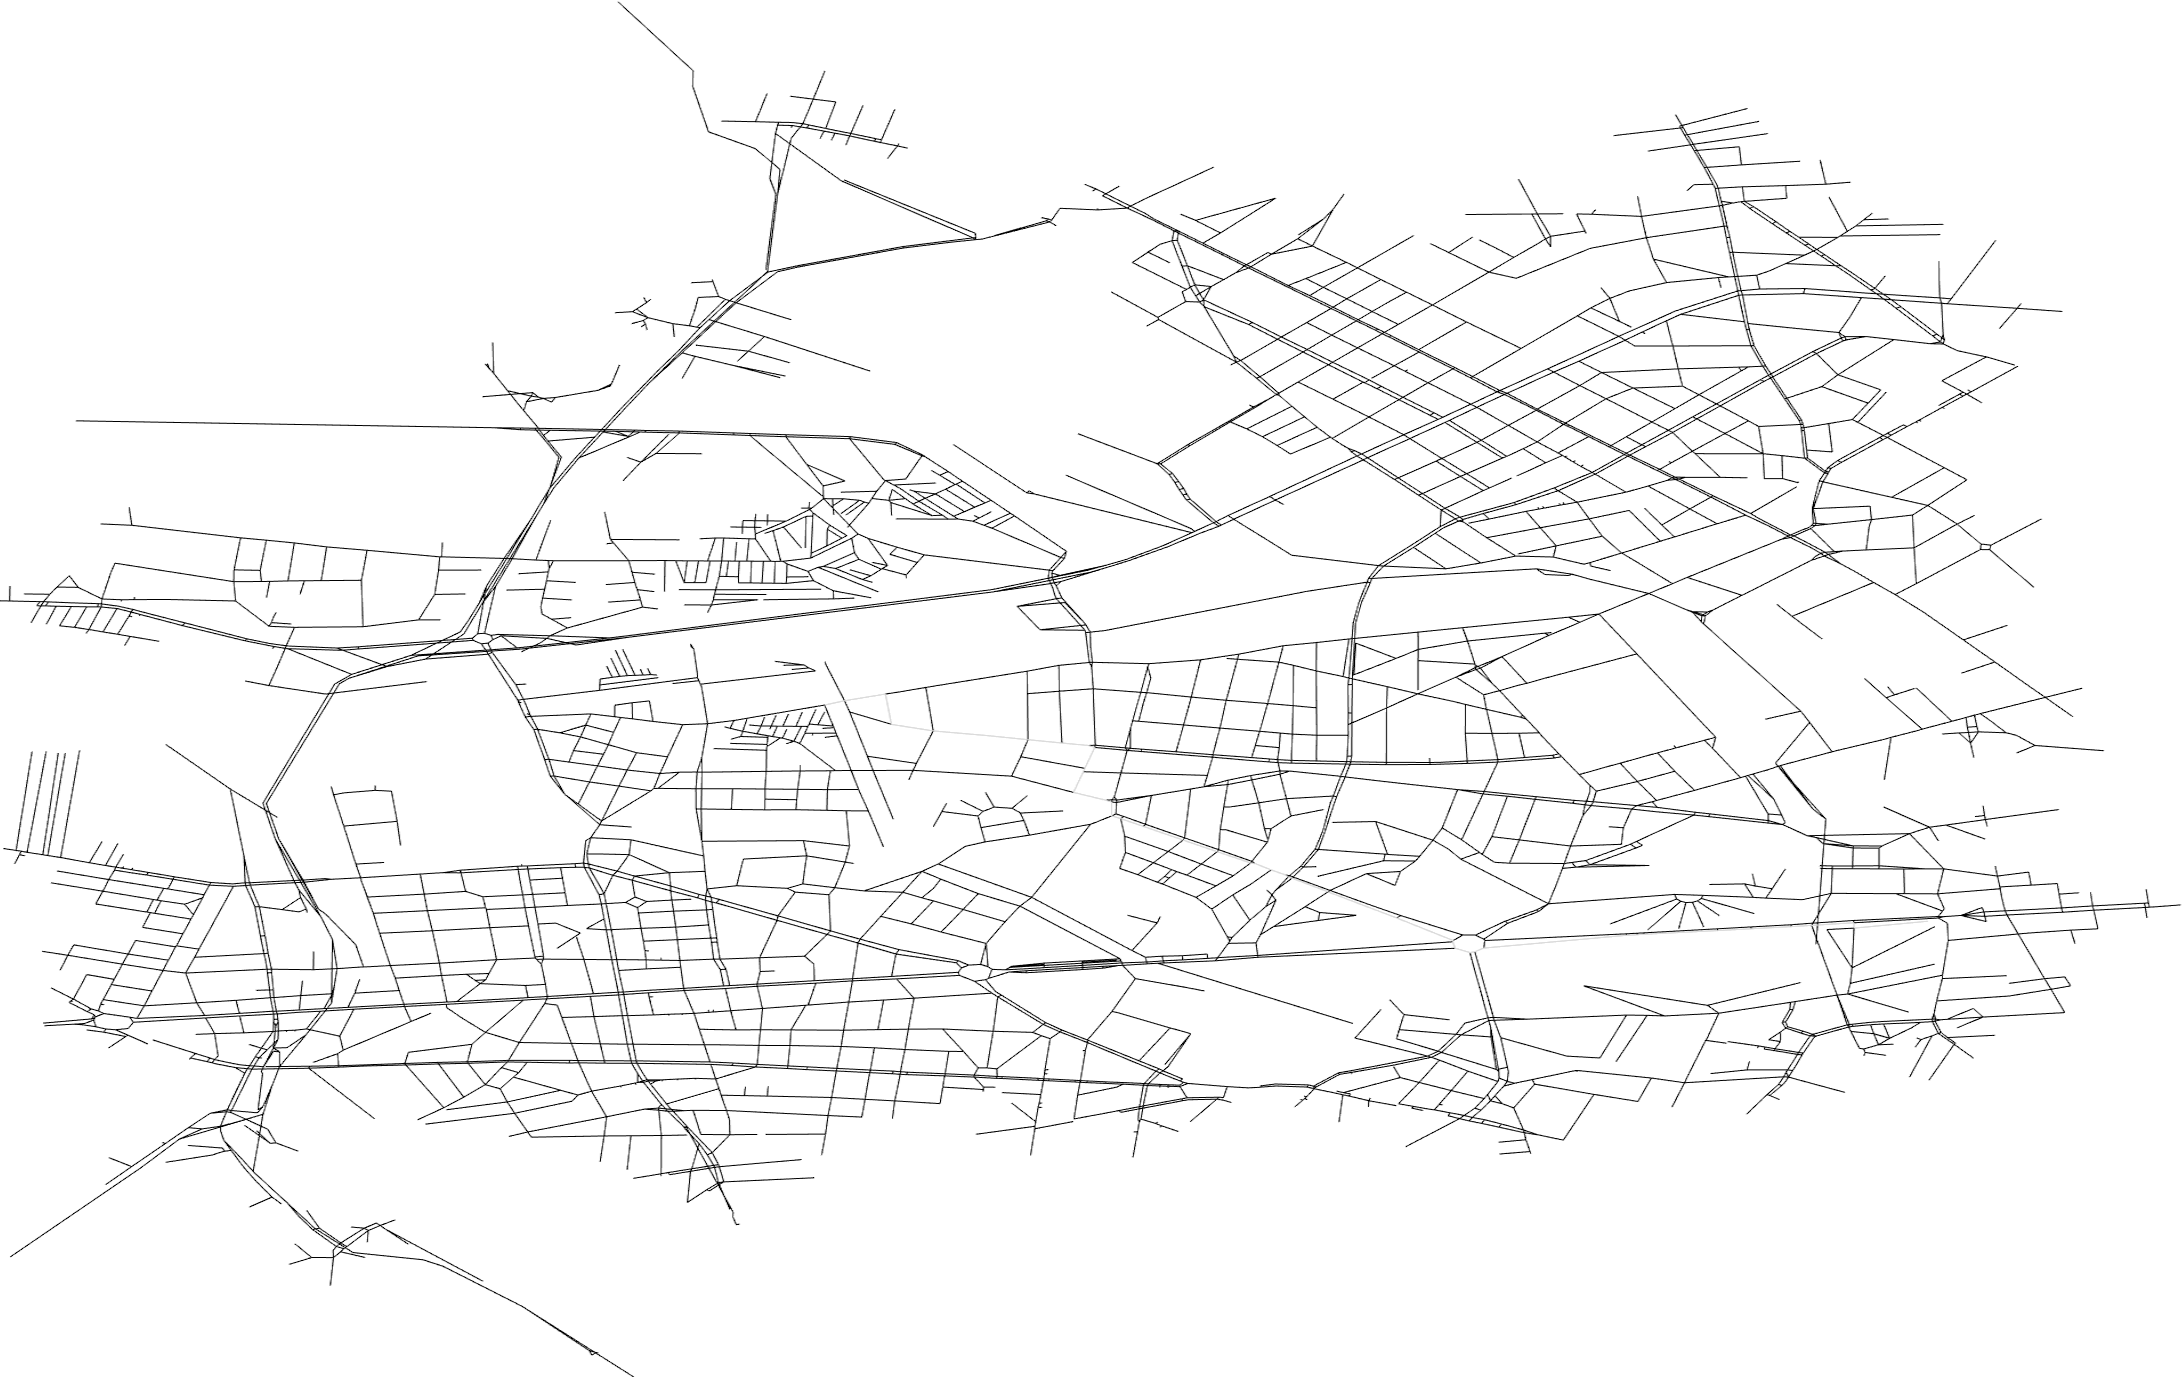
\includegraphics[width=\textwidth]{Images/vis-preprocessing-streched.png}
\caption[]{Preprocessing method with additional streching to the borders of the visualization}
\label{fig:spreaded_axis}
\end{figure}

As we see in \cref{fig:spreaded_axis} this reduces the unused space to a minimum.
Though we loose a lot of understandability, as the length of a line on the screen would indicate the length of the real edge even less.

As a result, we decided to use the preprocessing method with uniform axes for the visualization.
On the one hand, the additional performance costs in preprocessing are worth the reduced amount of unused space.
On the other hand, the possible unused space on one axis is worth the increased comprehensibility.


\subsection{Visualizing the Cache}

In this section, we will explain the way we figured out to display the cache in the visualization.
Taking the tiles as a foundation, we represent the cache by coloring the contained tiles.

\begin{figure}[H]
    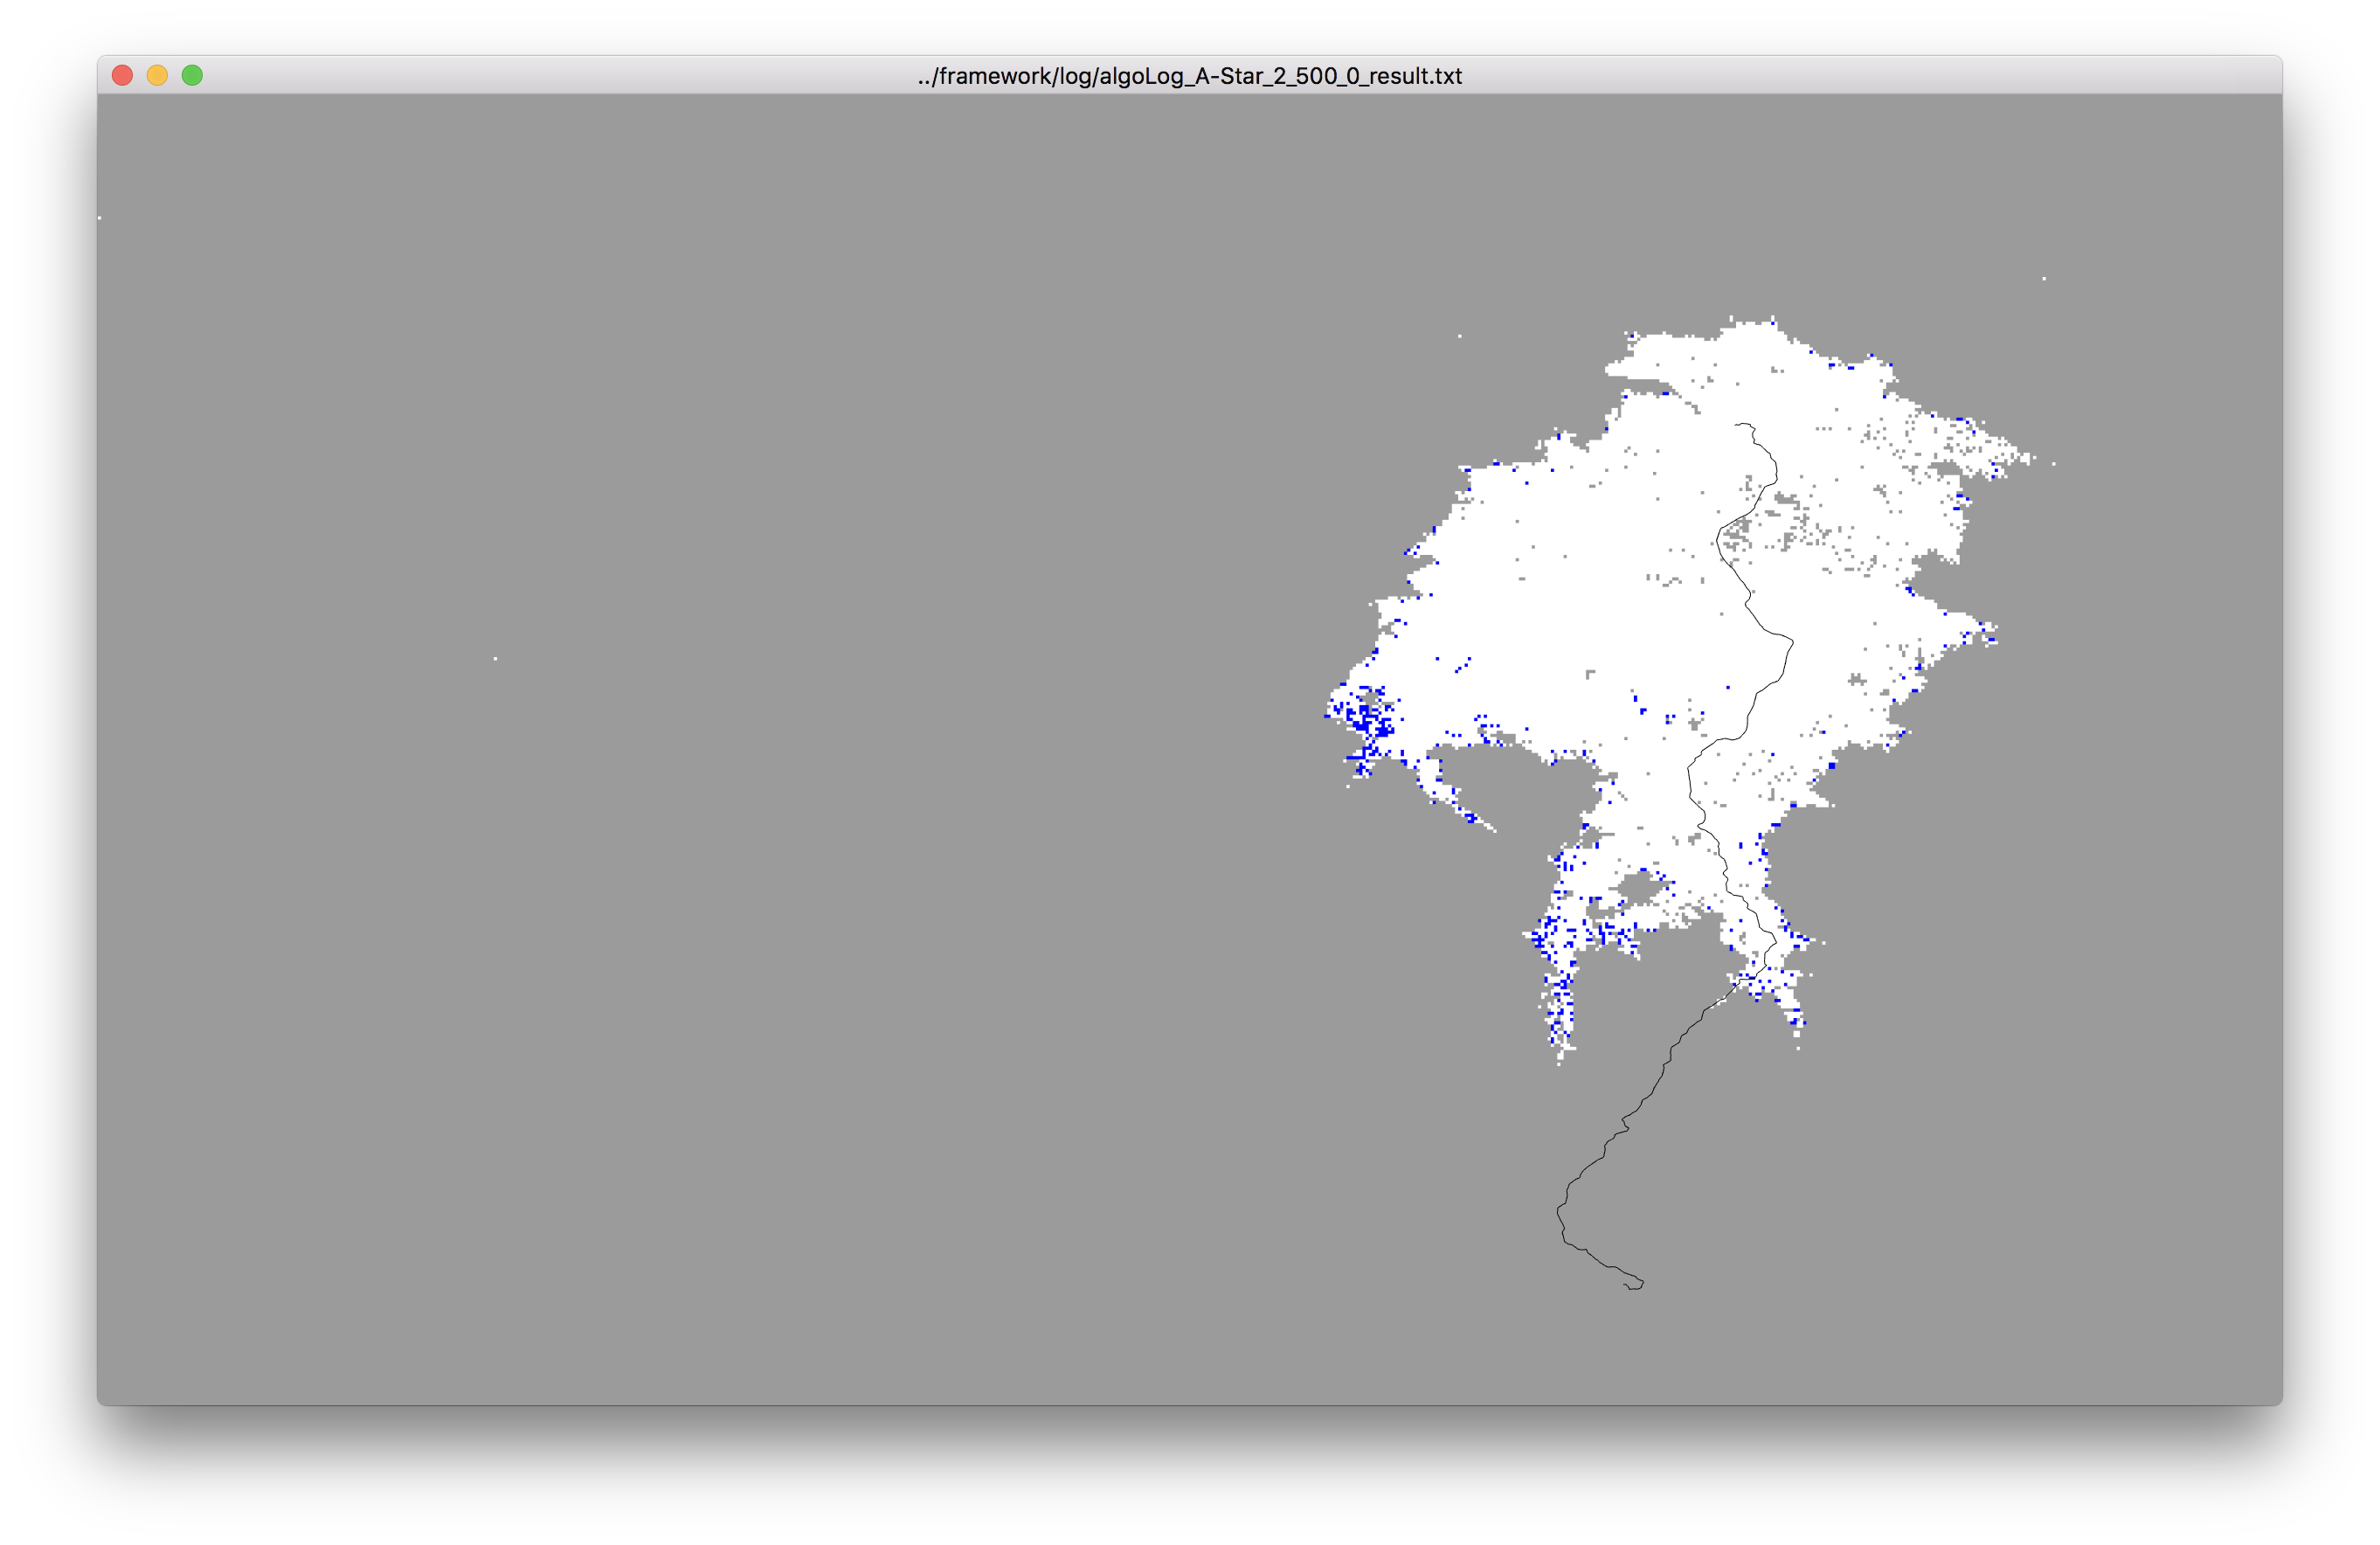
\includegraphics[width=\textwidth]{Images/vis-basic-cache.png}
\caption[]{Representing the cache. The cache is represented by the blue rectangular shapes.}
\label{fig:cache_coloring}
\end{figure}

In \cref{fig:cache_coloring} we can see, that we did not color the tiles based on their age anymore.
Due to the colored cache, we achieved an improved understanding of past loaded tiles and the aged based coloring would furthermore distract from the important cache.

For showing how well a framework performs, we color every tile, whenever it is not in the cache according to the frequency it has been loaded.

\begin{figure}[H]
    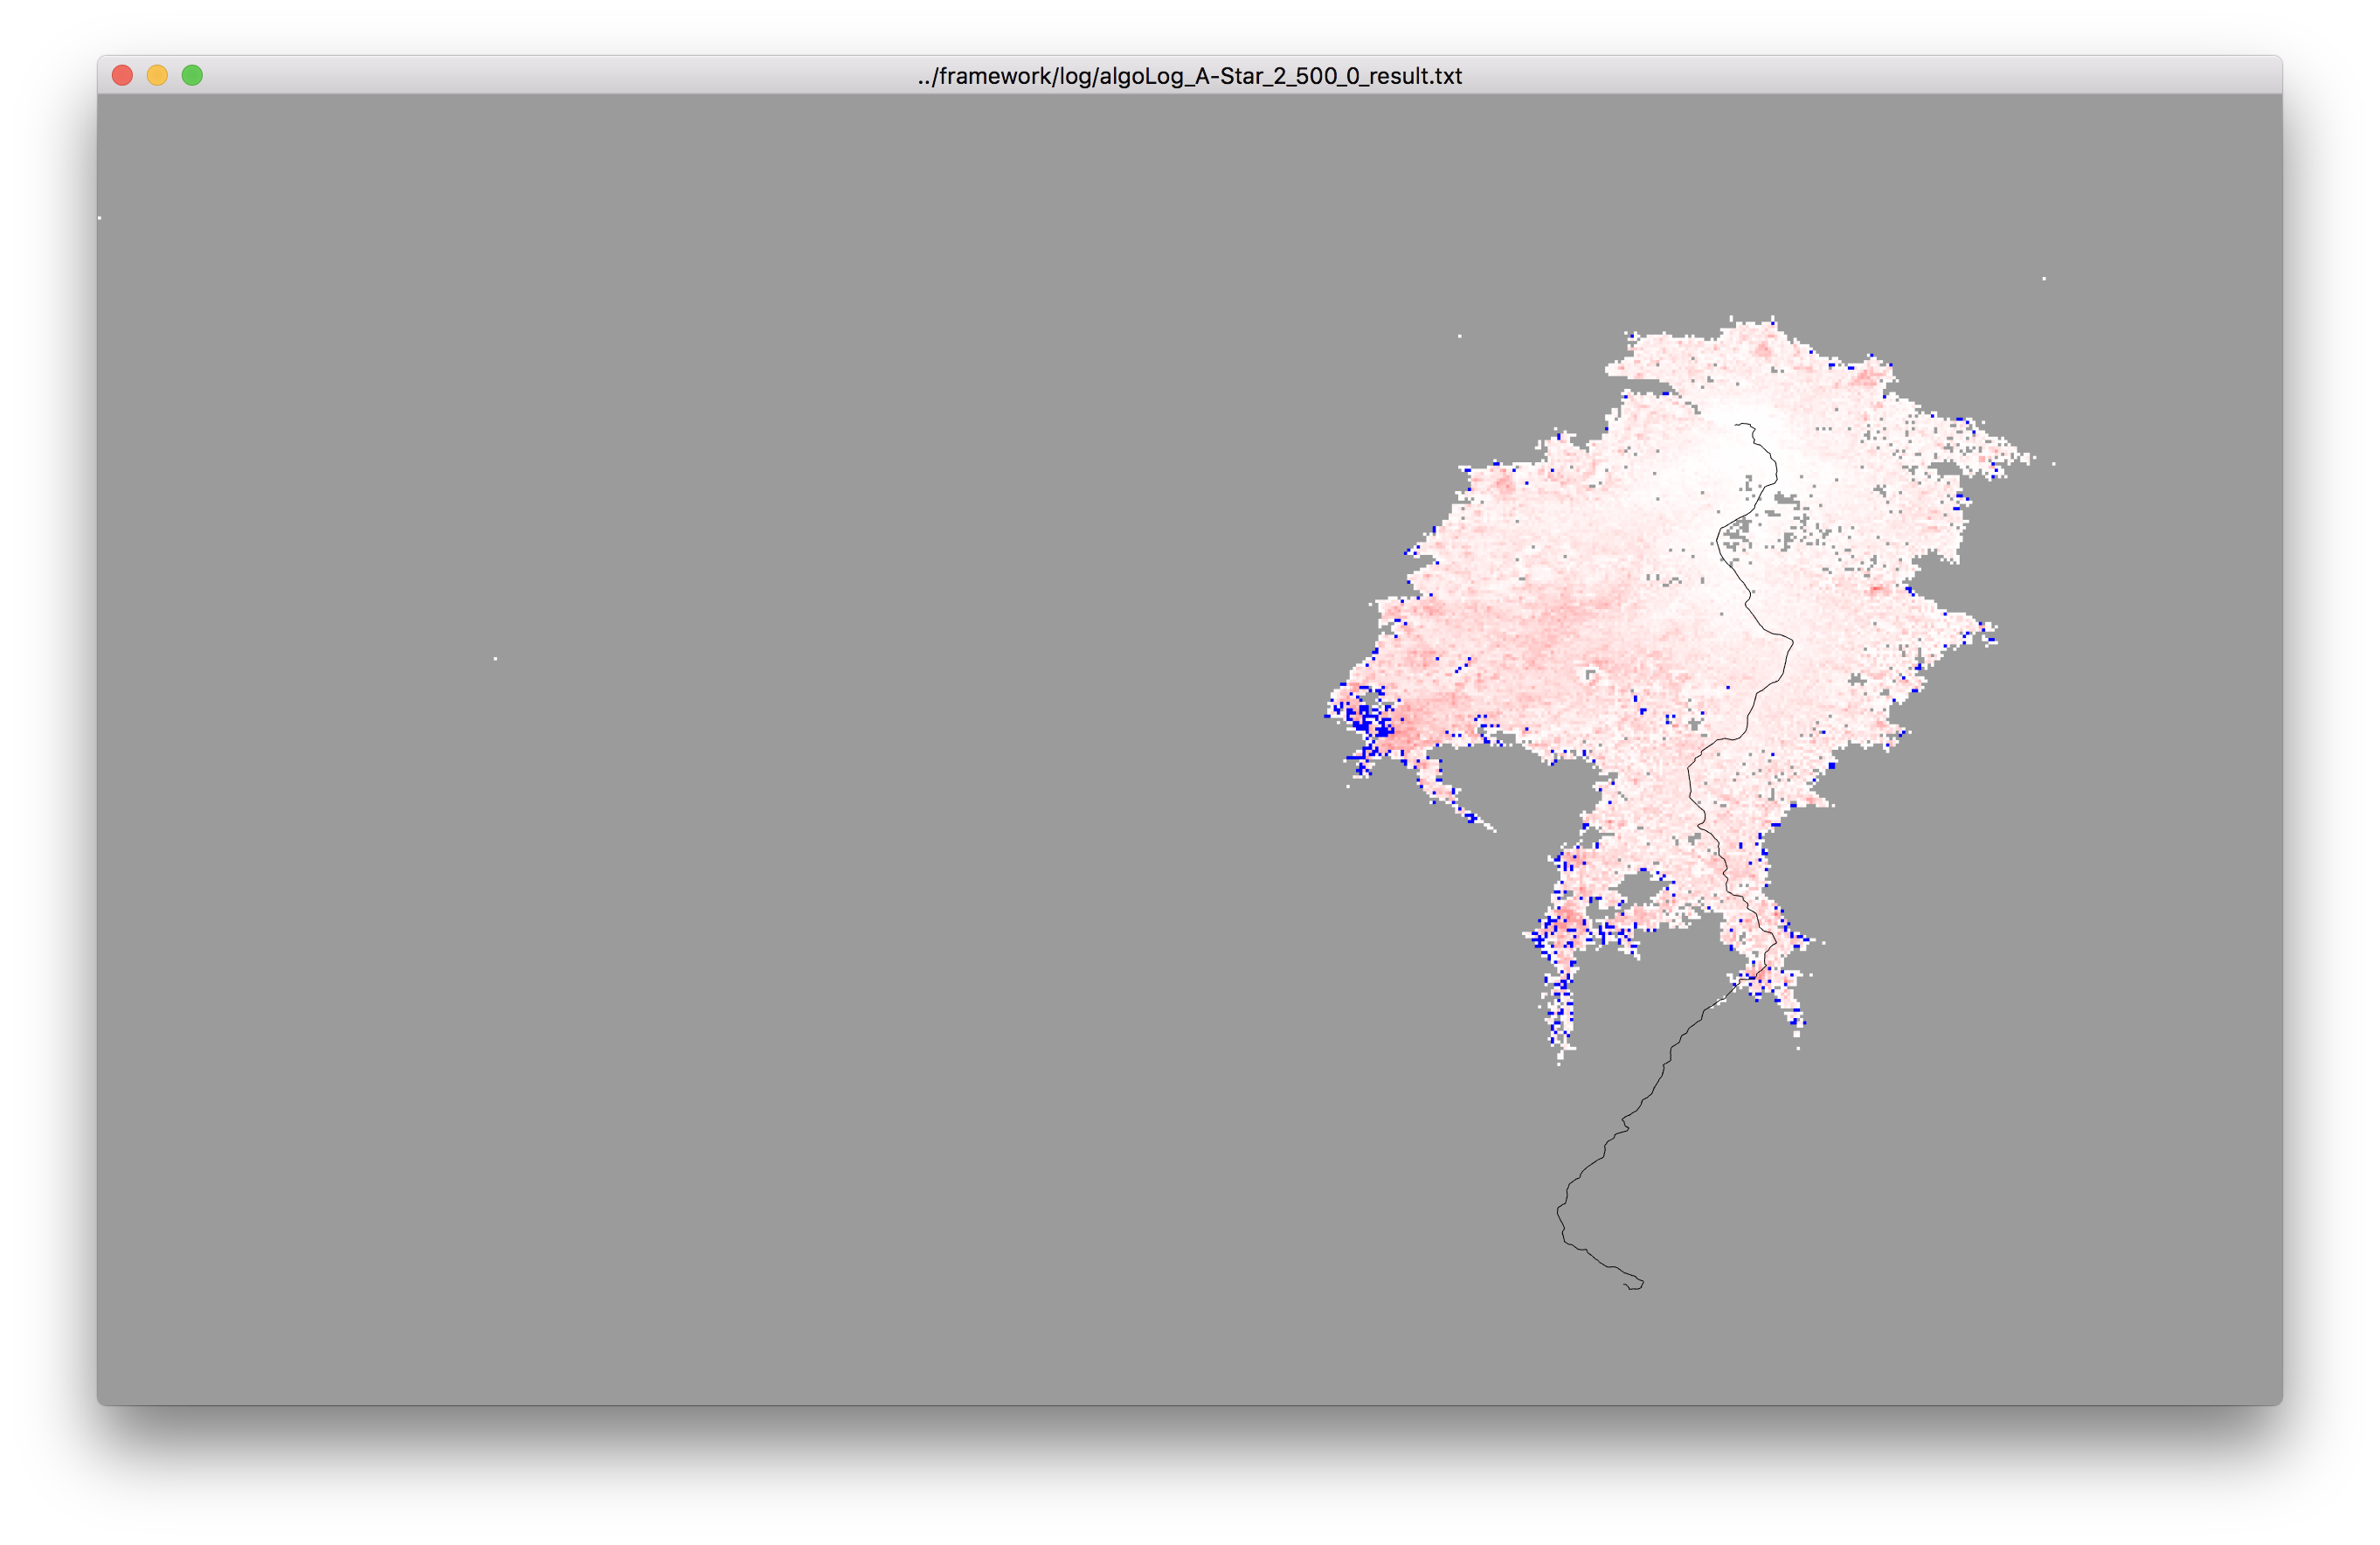
\includegraphics[width=\textwidth]{Images/vis-rgb-cache.png}
\caption[]{Coloring the tiles according to the amount of reloads. Red tiles has been loaded more often.}
\label{fig:reload_coloring_white}
\end{figure}

By coloring the reloads this way, we can now see how good our algorithm performs and in which regions more reloads occur.
With this color scheme, bigger differences in tile loading can be distinguished from each other easily.
Nevertheless smaller differences are hard to recognize.
Therefore, we tried another color scale.


By using a transition between two colors we hope to achieve a bigger and clearer contrast between slightly different tile loads.
We figured out that the HSV color space is a good choice whenever a transition between colors is wanted.
The HSV color space enables us to choose any color as a basis and then change the hue linear according to the amount of reloads.

\begin{figure}[H]
    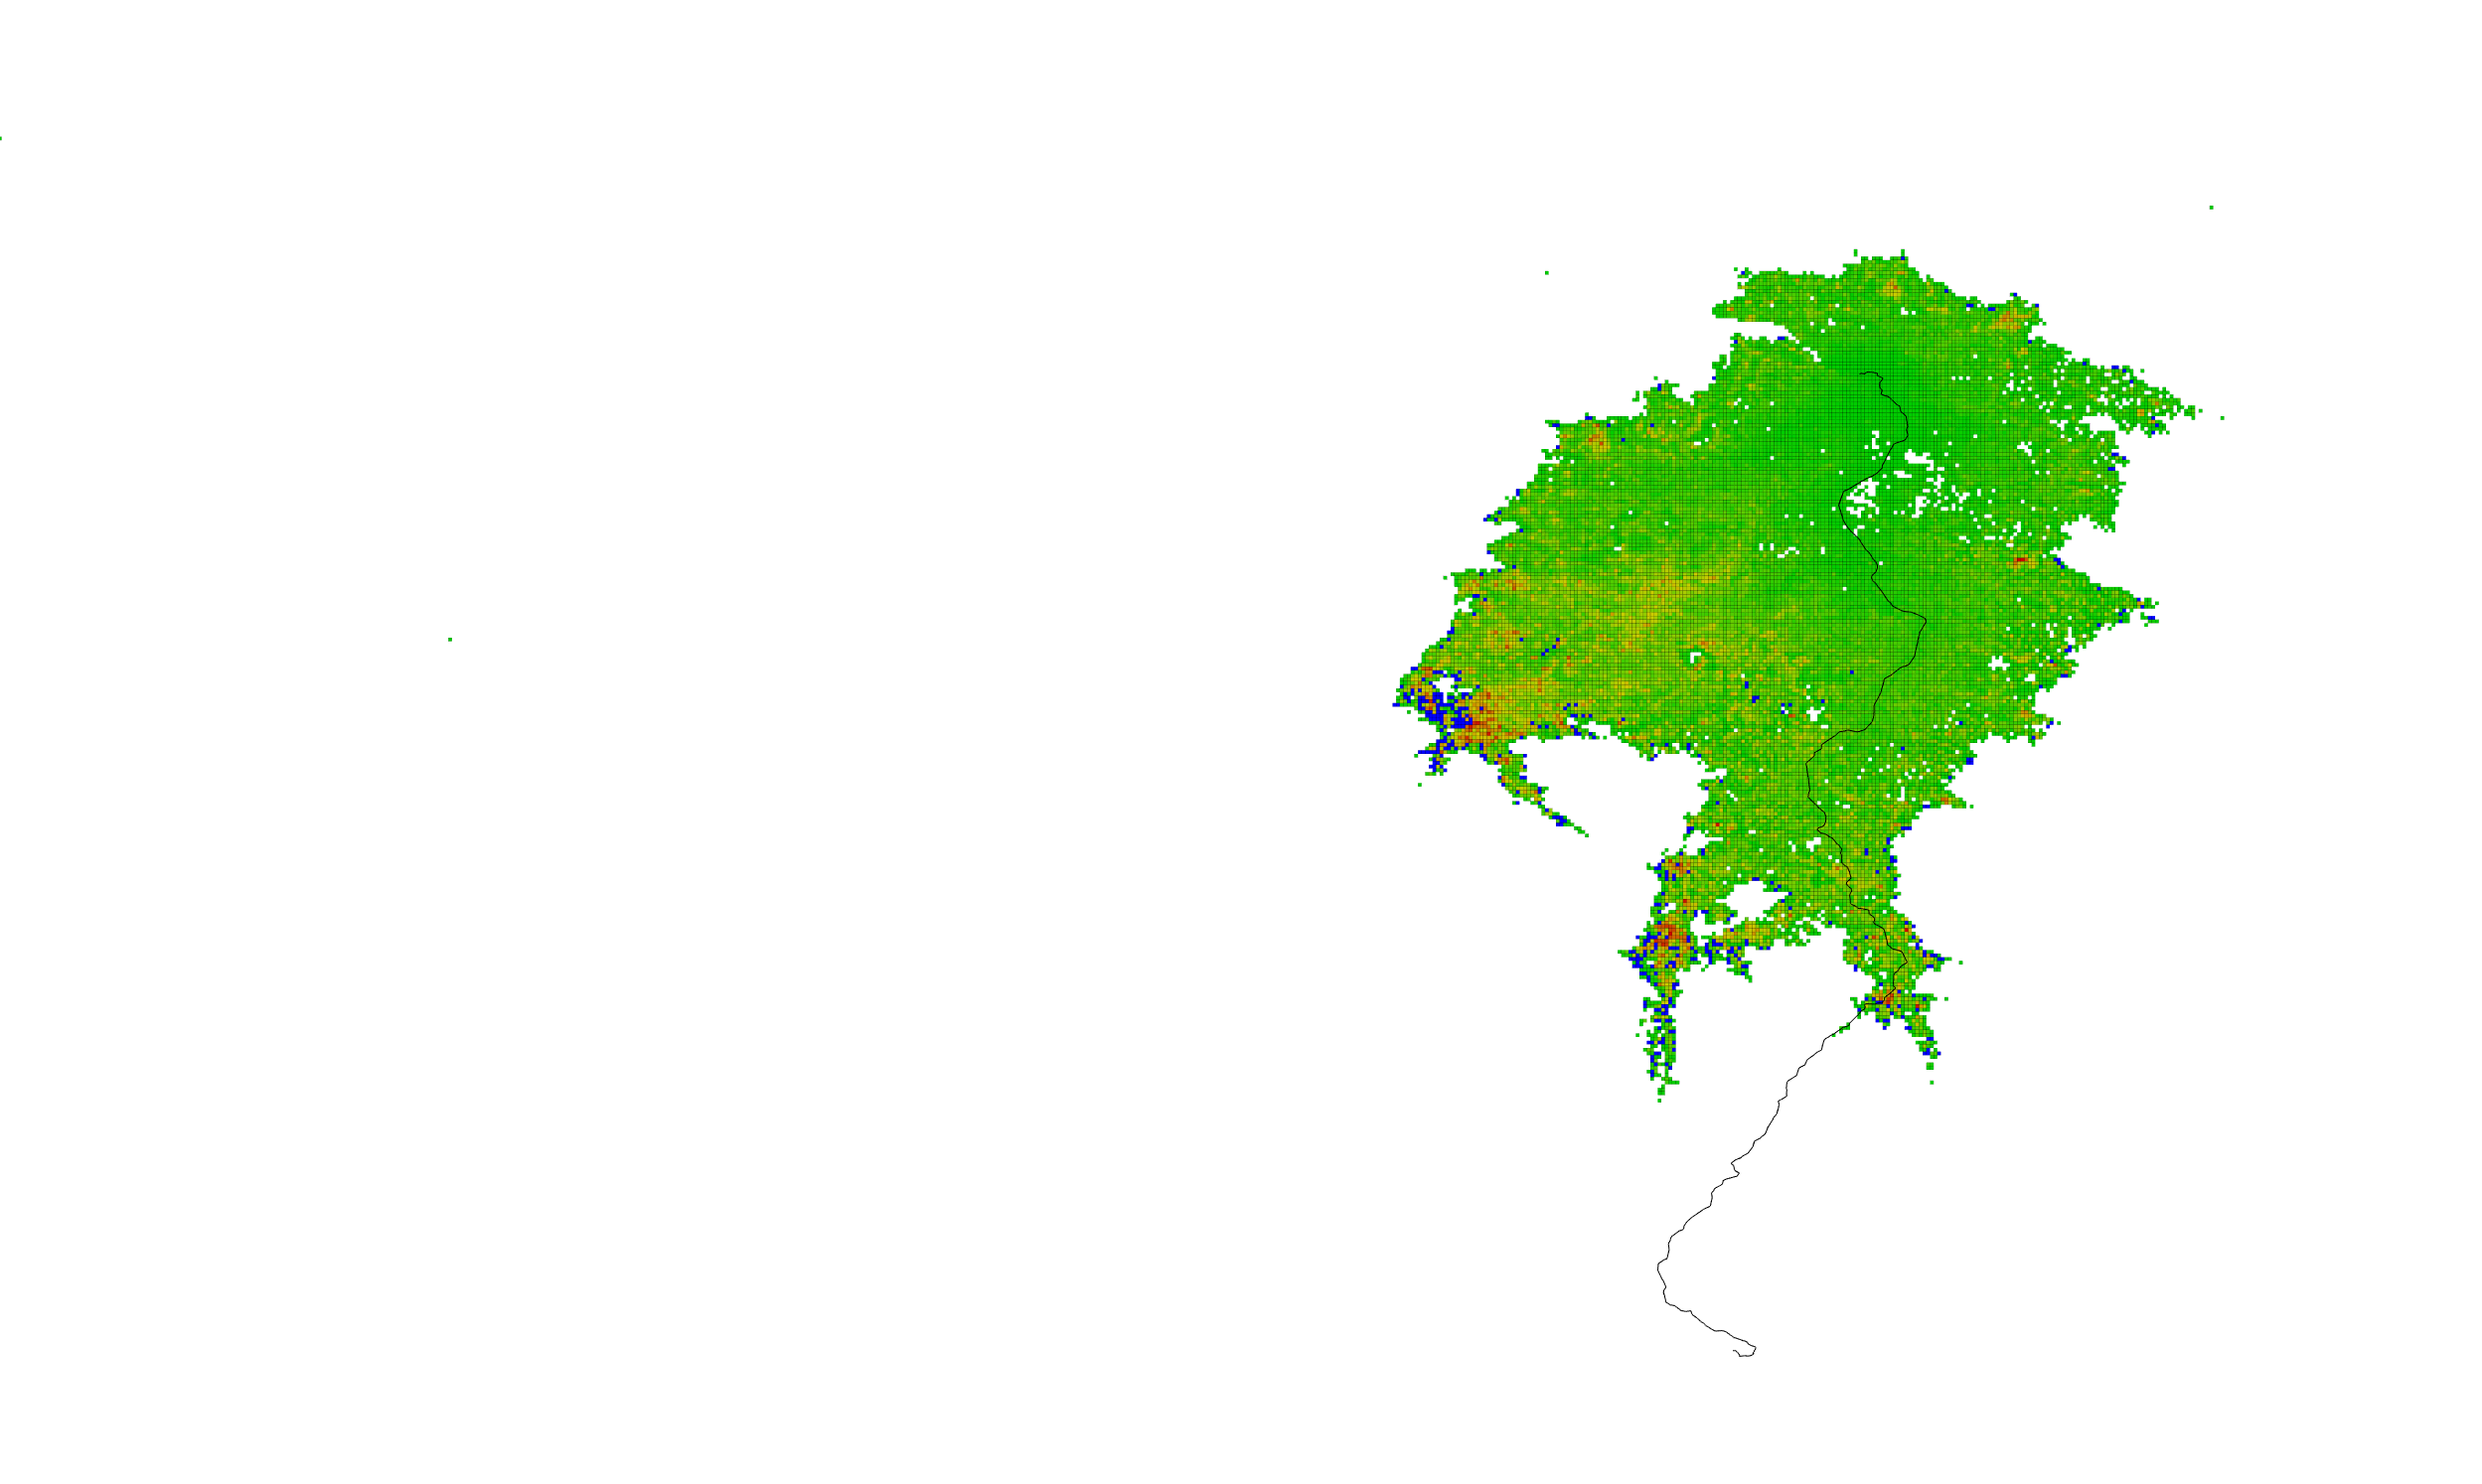
\includegraphics[width=\textwidth]{Images/vis-hsv-cache.png}
\caption[]{Changed color scheme. Now the tiles change their color from green to red.}
\label{fig:reload_coloring_hsv}
\end{figure}

In \cref{fig:reload_coloring_hsv} we see the differences between two similar values clearer than in the transition from an uncolored tile to a specific color.
As a side effect, the graph distinguished from the background much better now and the visualization look much better.

\section{Compare algorithms} \label{compare}

A first approach for comparing two versions of the framework is to simply start two visualizations and display them next to each other.

\begin{figure}[H]
    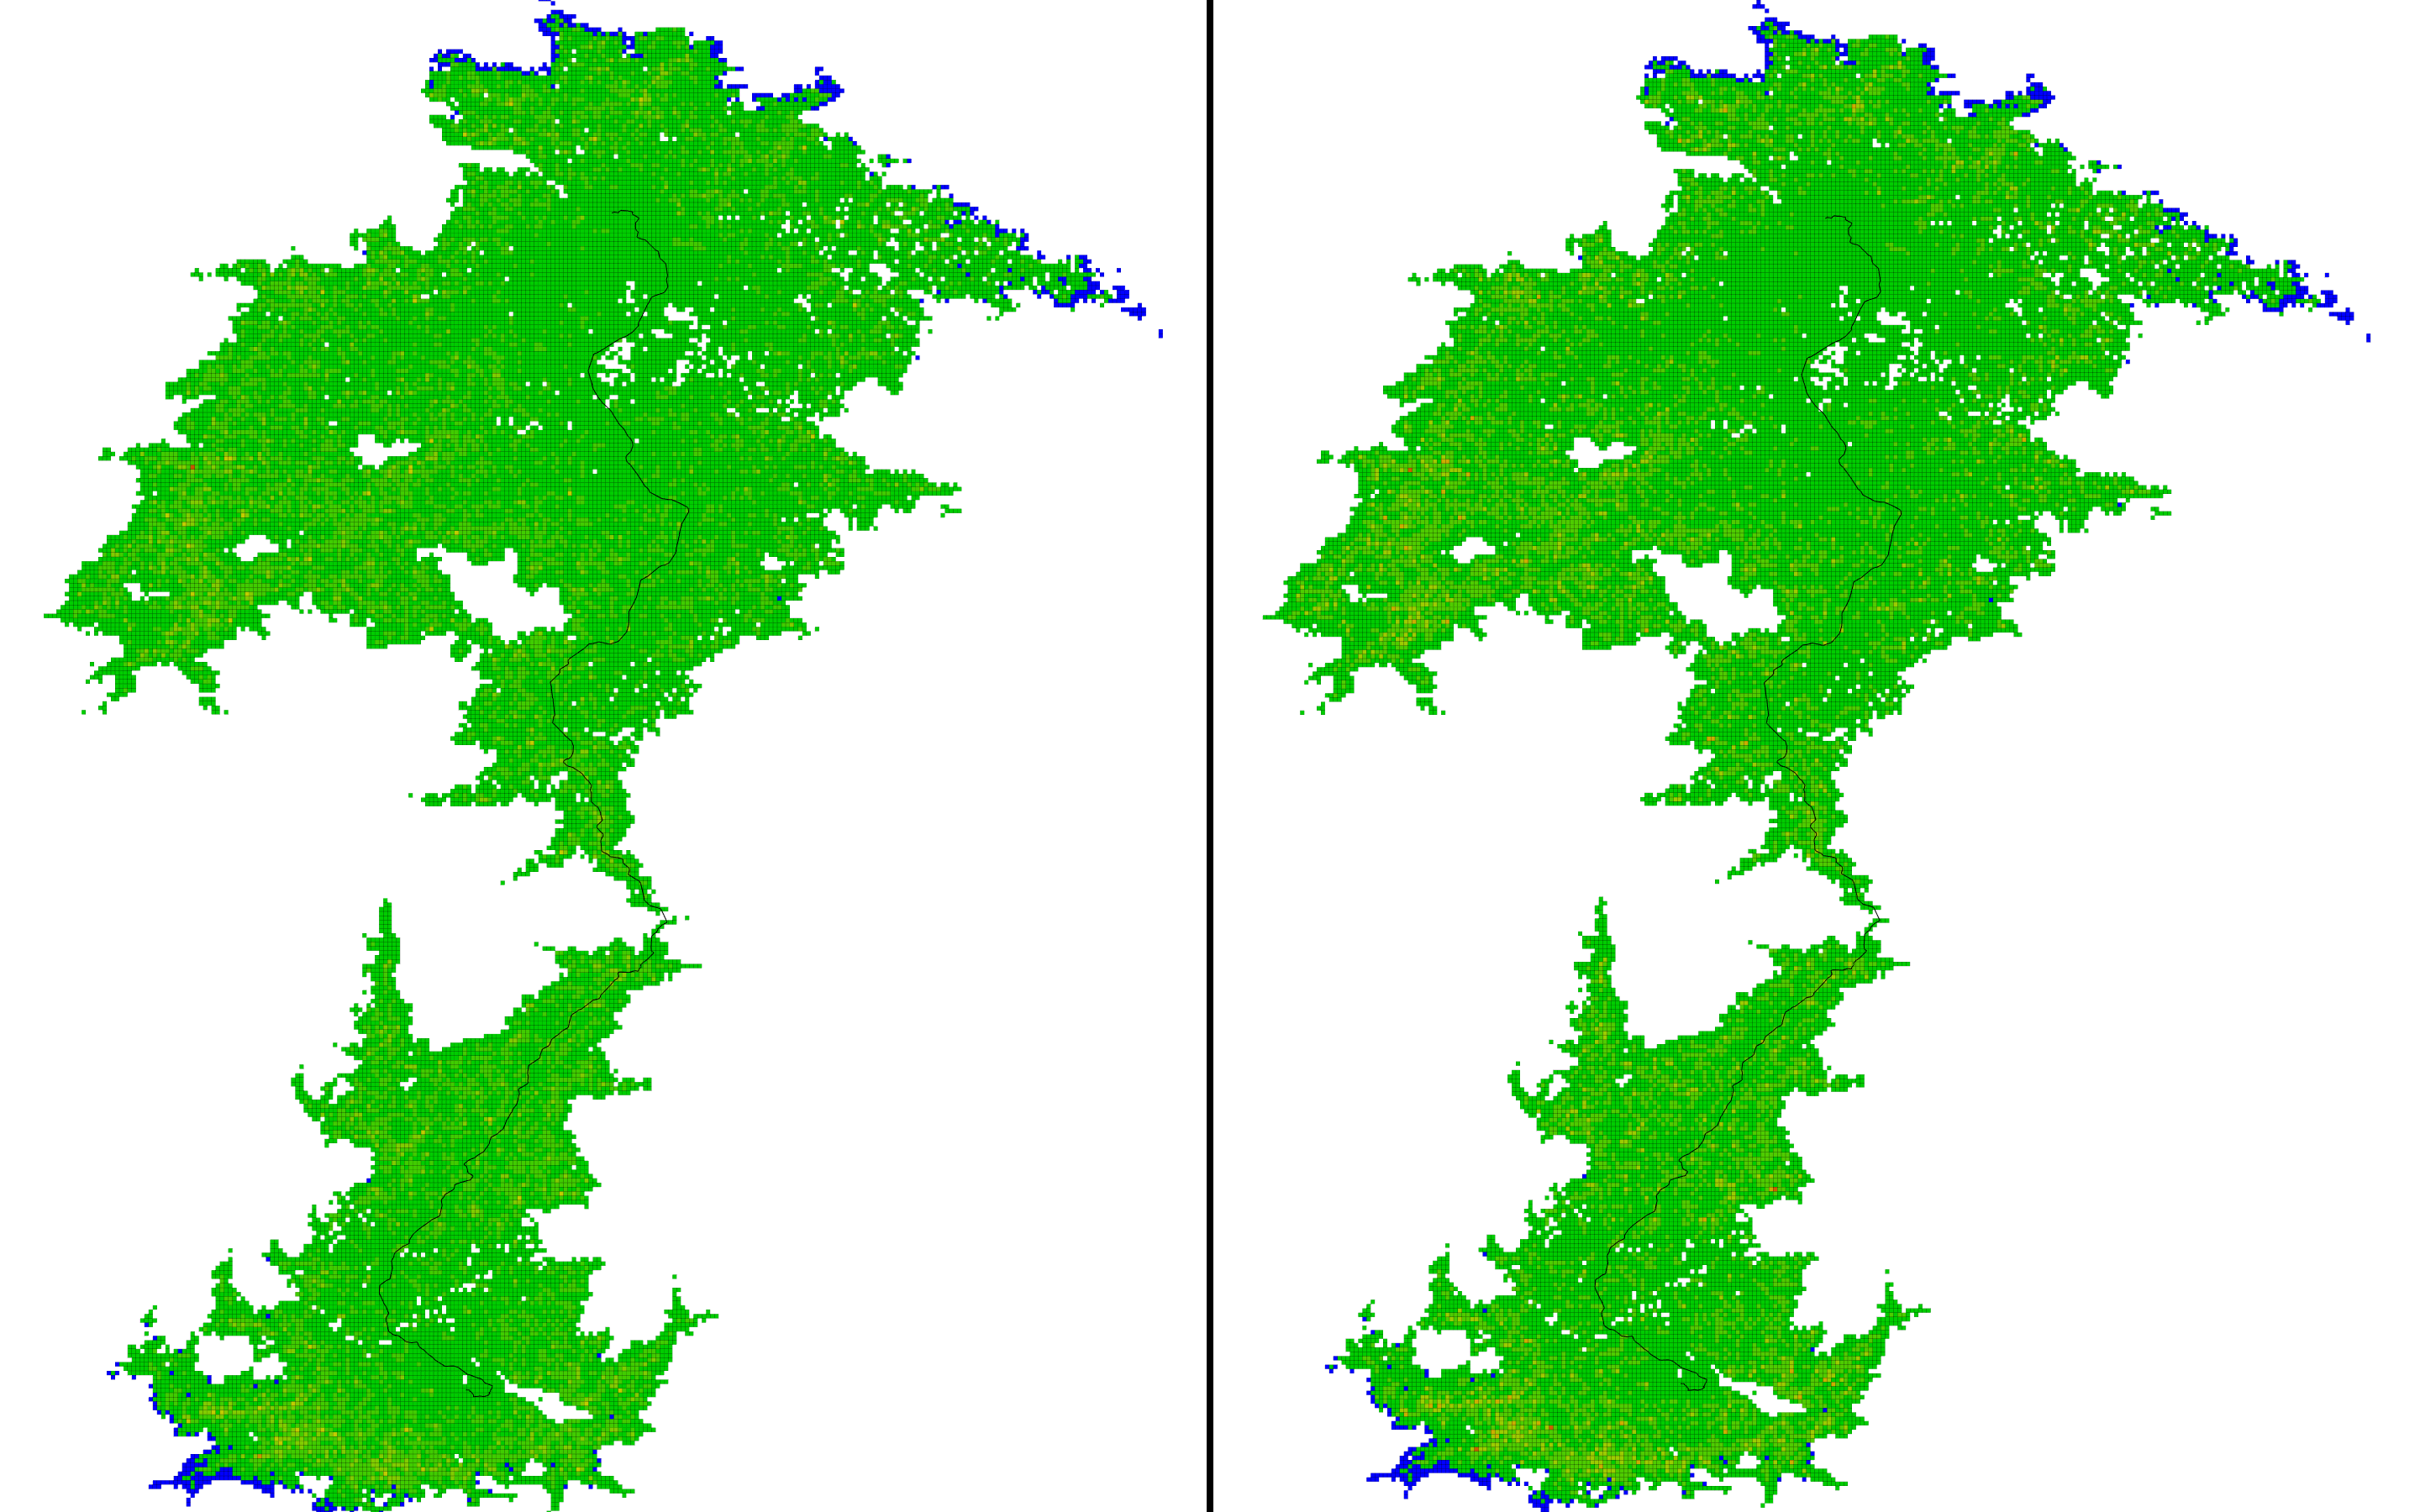
\includegraphics[width=\textwidth]{Images/vis-compare-two.png}
\caption[]{Running two visualizations next to each other.}
\label{fig:two_visualization}
\end{figure}

In \cref{fig:two_visualization} we can see no big difference between the two algorithms.
We experienced that this kind of comparison is only useful for algorithms which differ in the tiles that has been loaded or have bigger differences in the amount of tile loads.
For comparing algorithms with small differences we, therefore, developed a new variation of the visualization.
Therefore we removed the space between both visualizations.
The idea is, that smaller differences are better visible when tiles with the same location are displayed directly next to each other.
Therefore we split each tile in two and color the left half according to the reloads of one algorithm and the right half according to the reloads of the other algorithm.

\begin{figure}[H]
    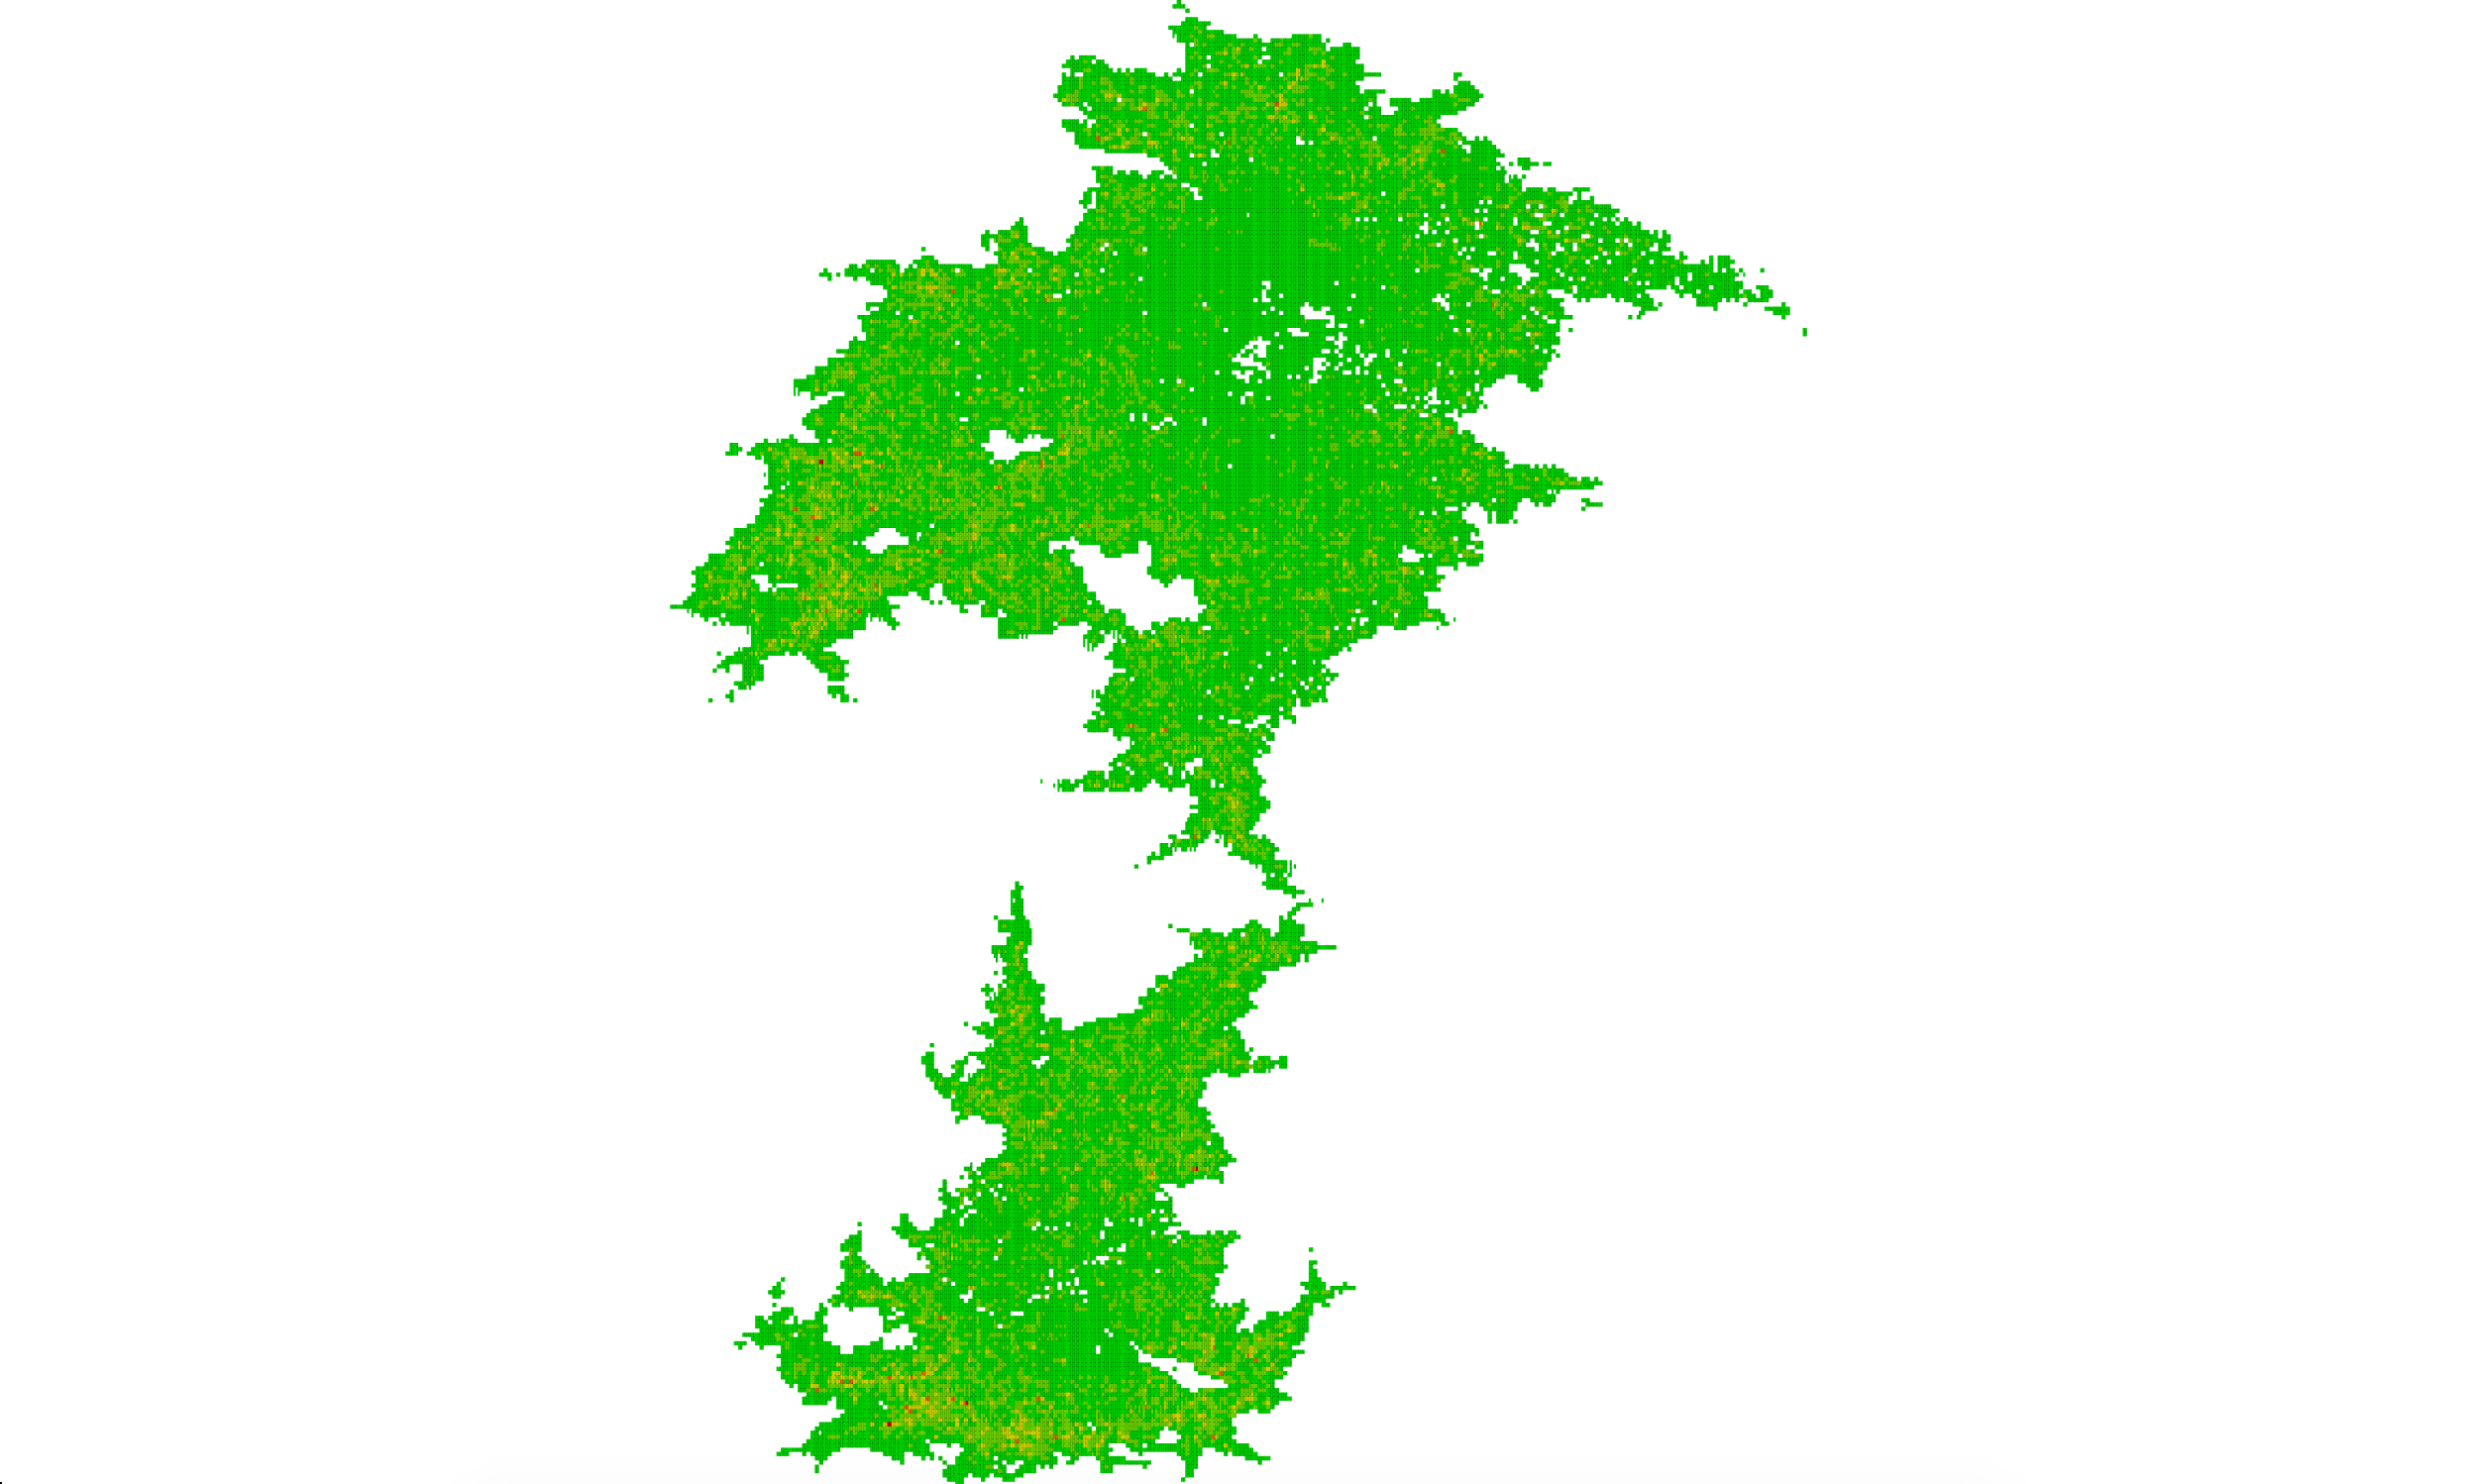
\includegraphics[width=\textwidth]{Images/vis-compare-splitted.png}
\caption[]{Splitting the tiles.}
\label{fig:splitted tiles}
\end{figure}

This method provides a better way to see differences that affect only a few tiles, as we can see in \cref{fig:split tiles}.
However, it is still difficult to clearly identify the differences without longer observation, as it is hard to associate a tile half to one of the frameworks.
At this point, we could expand this method to label the algorithms with different colored outlines of the tiles, but as we are only interested in the differences between algorithms, when comparing them, we developed an approach that is only showing the difference between the tile loads.

This method calculates the difference between the amount of tile loads from both algorithms for each tile.
Then it displays all the tiles that have been accessed by at least one algorithm and colors those bluish that have been loaded more often by the first algorithm.
Those that have been loaded more often by the second algorithm are colored reddish.
The more intense the color, the bigger is the difference in the amount of tile loads.

\begin{figure}[H]
    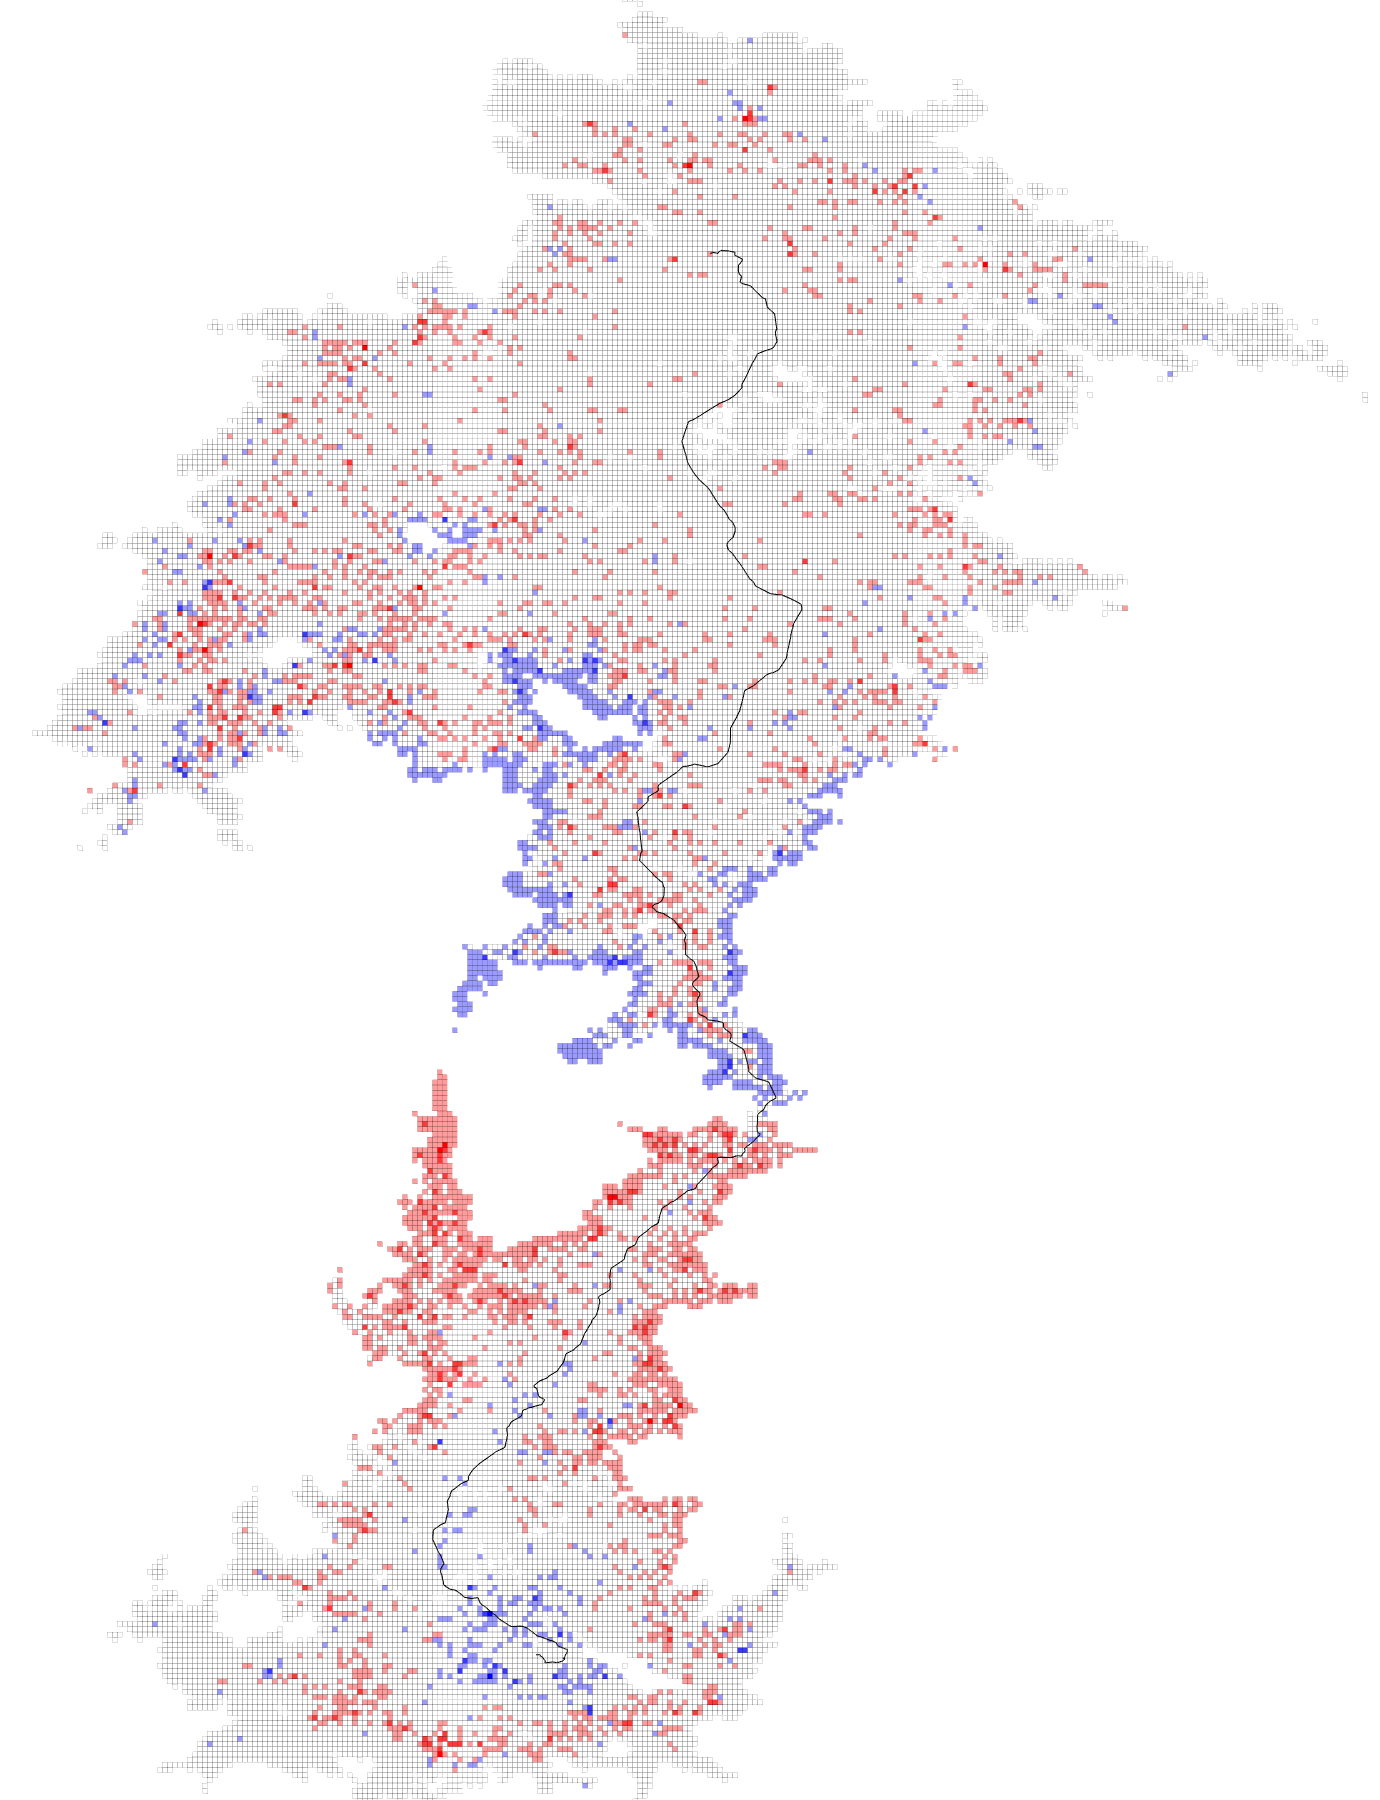
\includegraphics[width=\textwidth]{Images/vis-compare-colored.png}
\caption[]{Showing only the difference of tile loads.}
\label{fig:difference}
\end{figure}

In  \cref{fig:difference} we can now see that both algorithms are similar for most tiles.
Still, there are many tiles that are loaded more often by the second algorithm and even some for which the first algorithm performs better.


\section{Miscellaneous}

In this section, we will take a look on the visualization we have just build and think about some additional features.
For routes with a bigger distance, as for example in \cref{fig:reload_coloring_hsv}, we had to realize, that even the high-level visualization, that displays only the tiles, has the issue that single elements, as in this case the tiles, become quite small.
Therefore we added a zoom feature to the visualization.
After having implemented this it was necessary to enable a way to navigate in the graph as well, as otherwise we would be stuck in the middle of the graph.

\begin{figure}[H]
    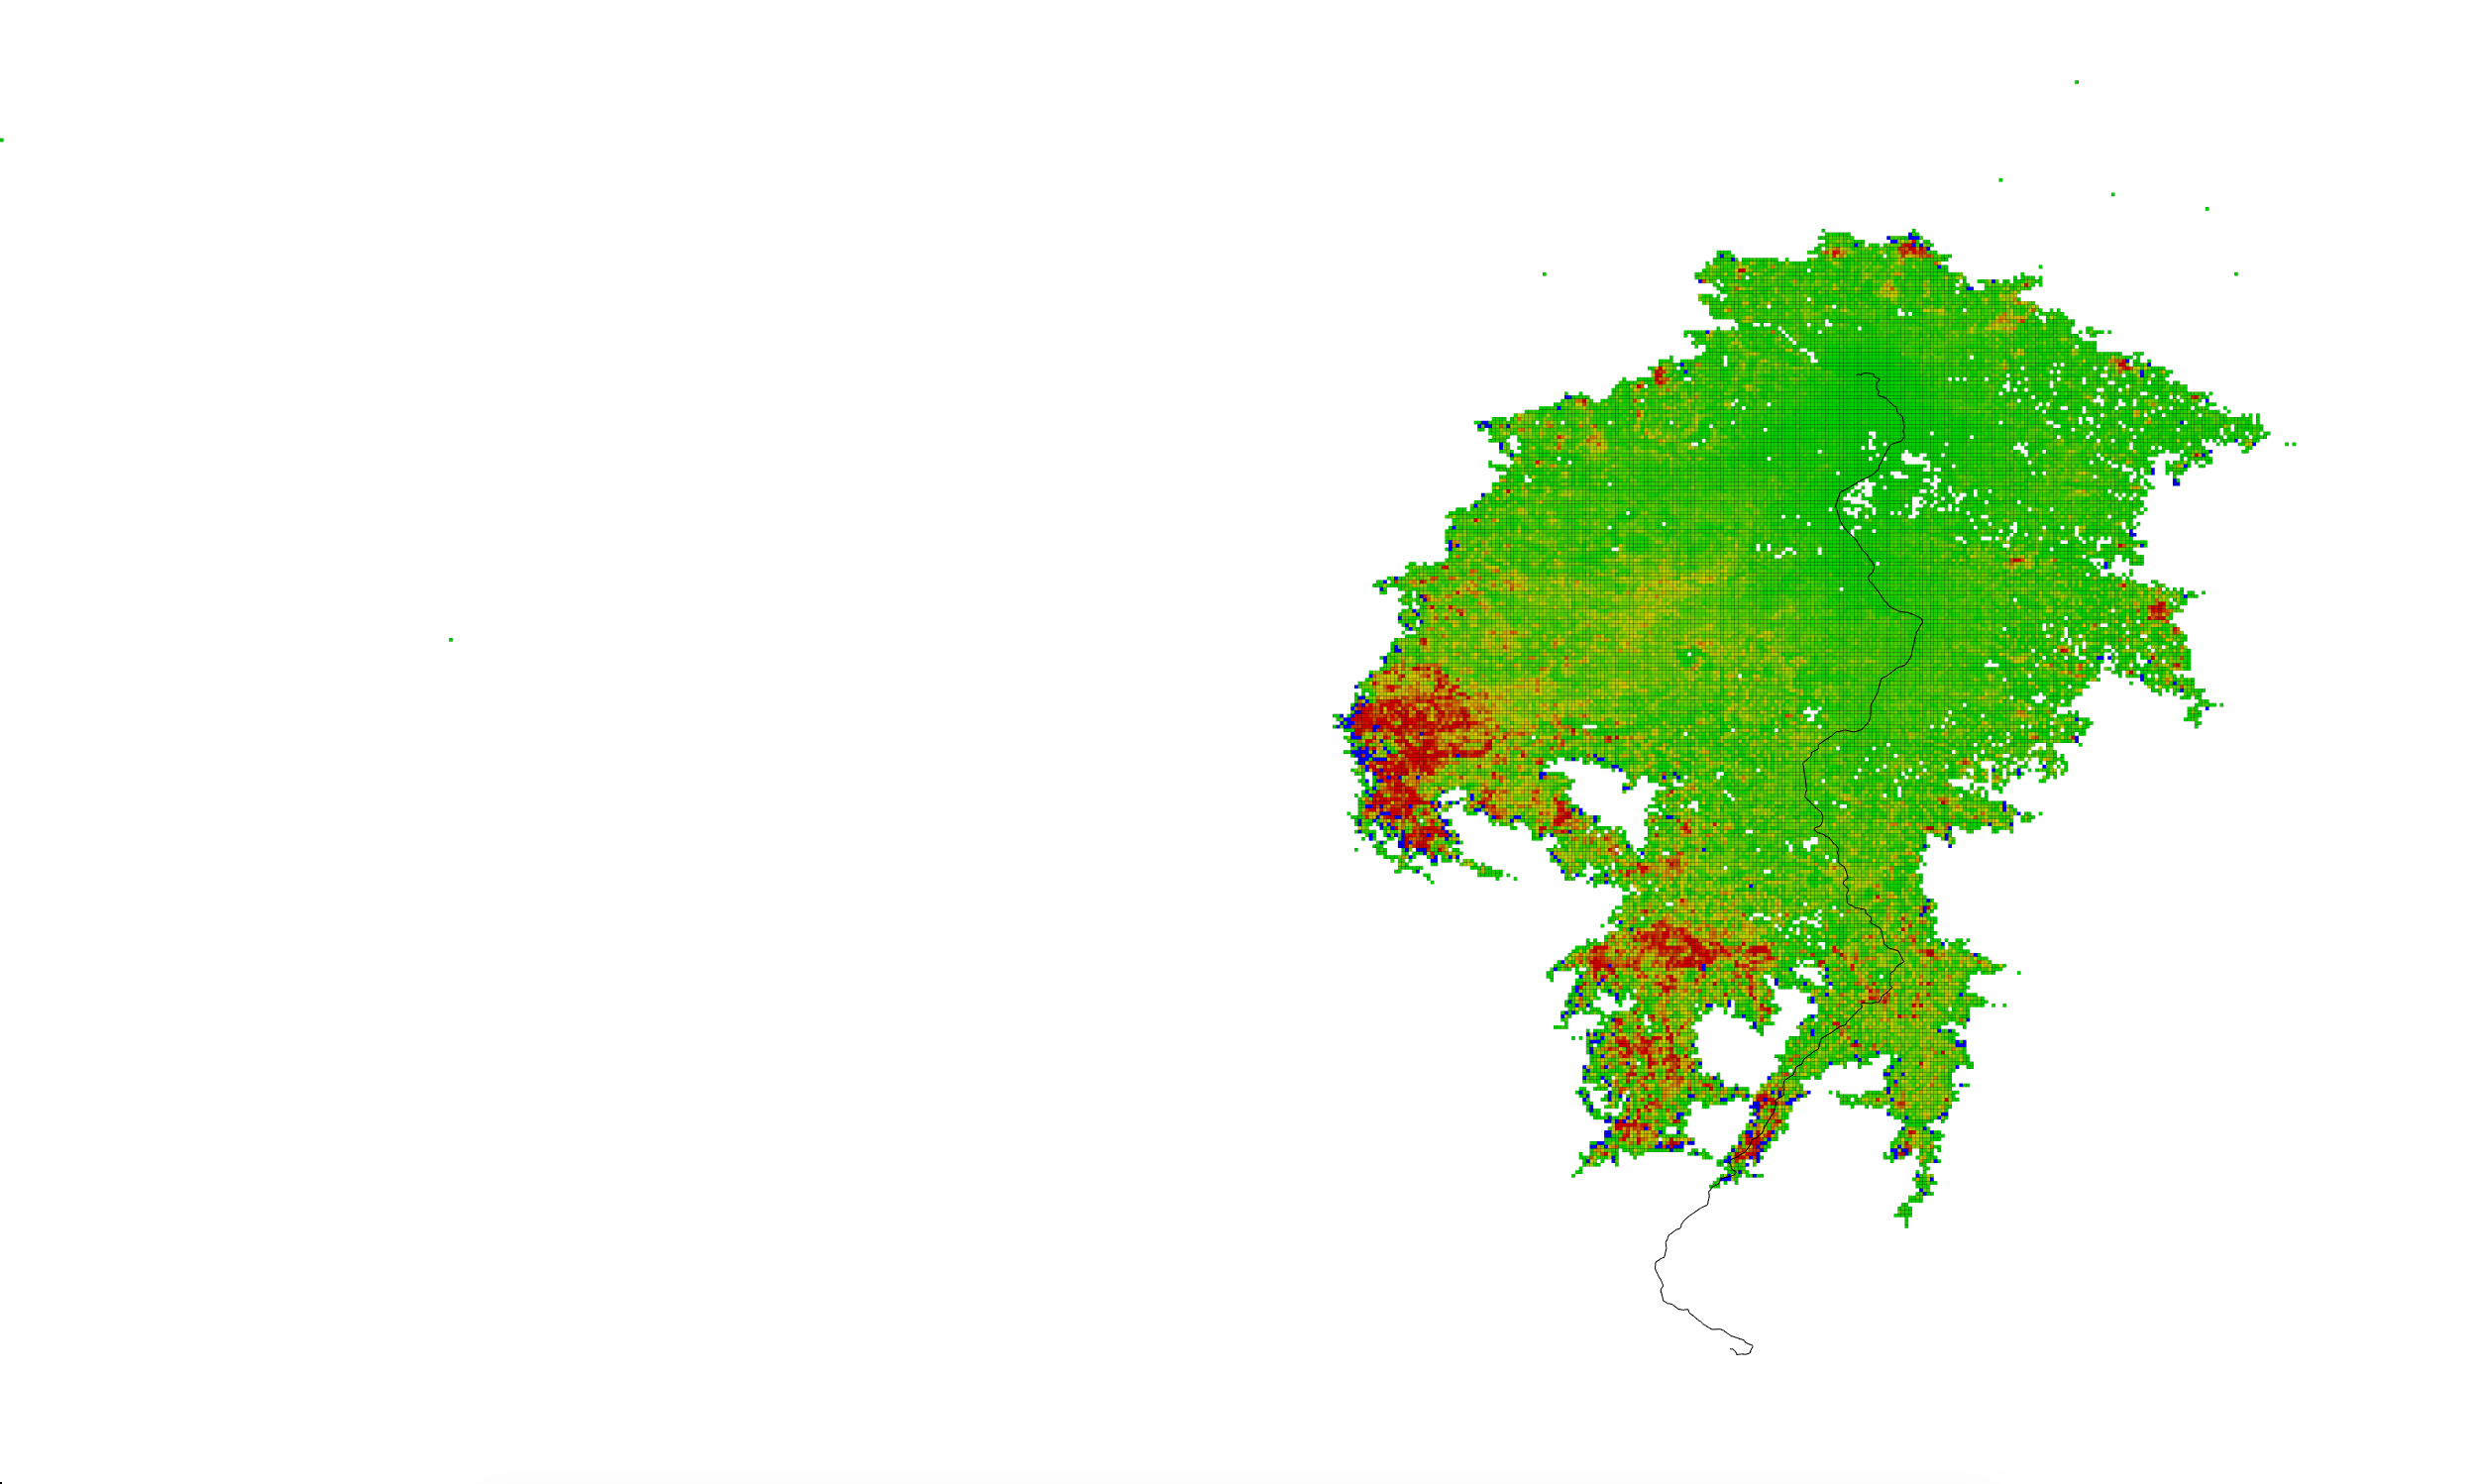
\includegraphics[width=0.5\textwidth]{Images/vis-zoom-small.png}
    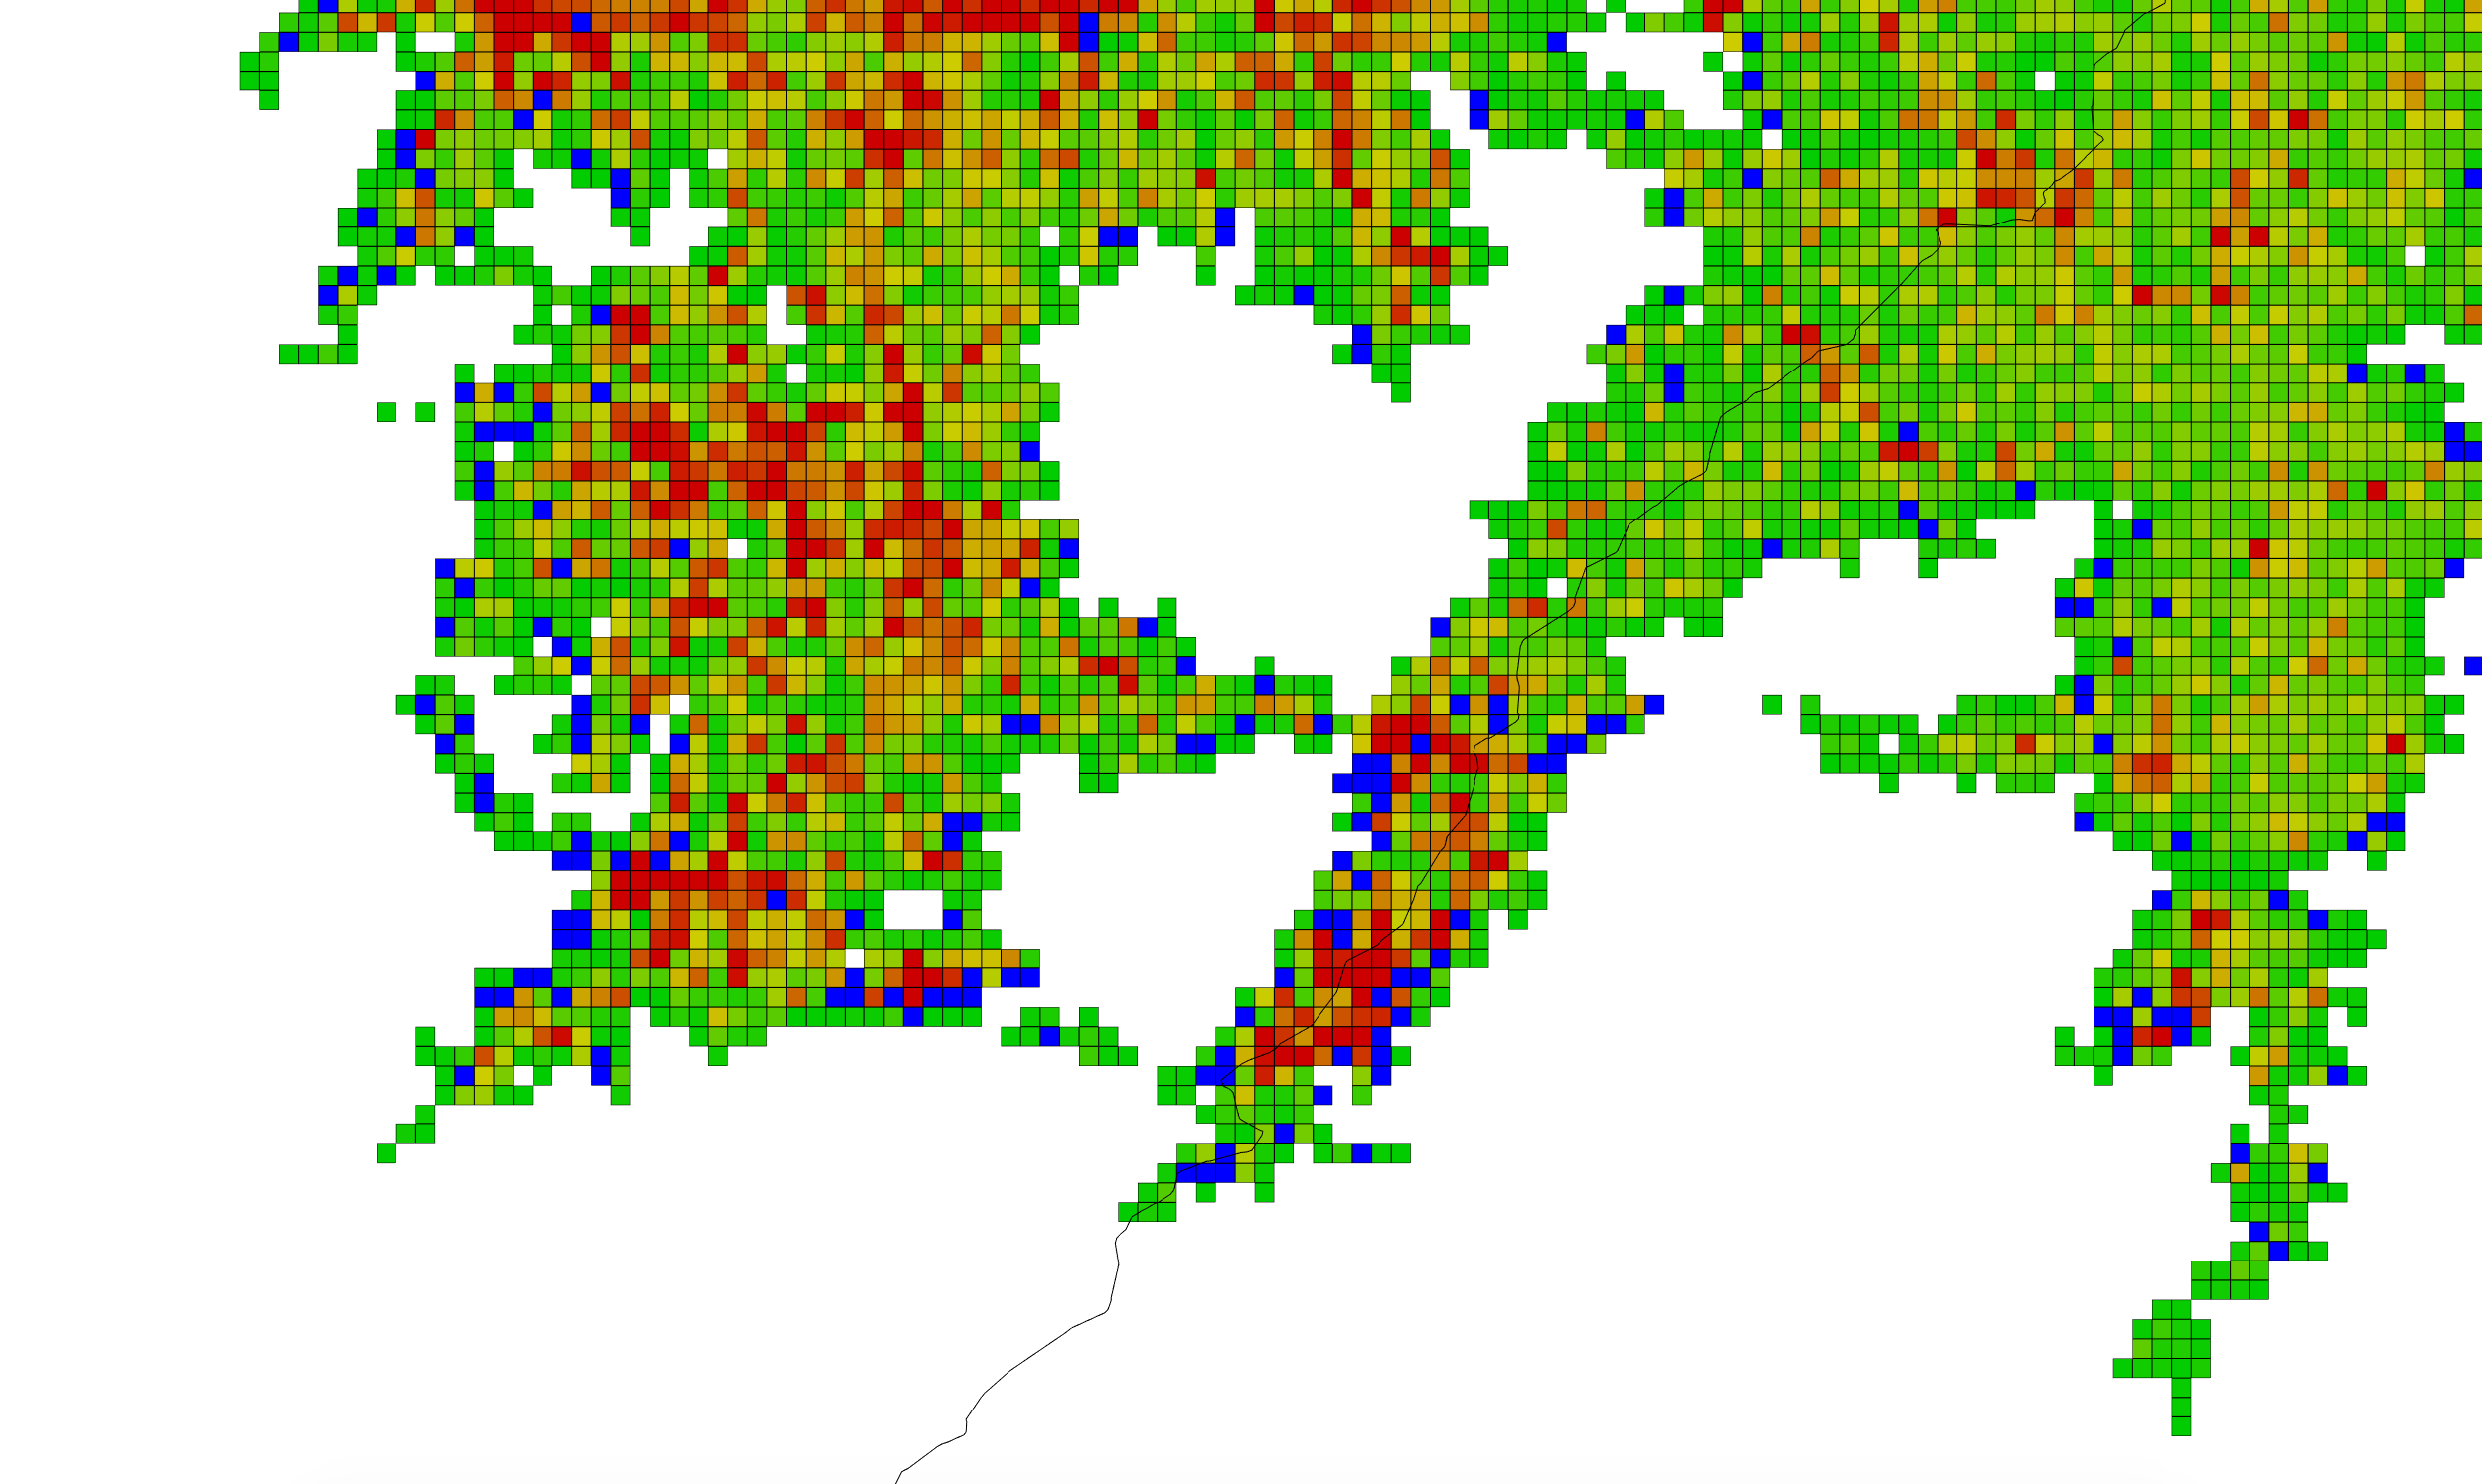
\includegraphics[width=0.5\textwidth]{Images/vis-zoom-large.png}
\caption[]{View on whole graph(left) vz Zoomed view(right)}
\label{fig:zoom}
\end{figure}

We are now able to have a more detailed view on smaller parts of the graph, as we see in \cref{fig:zoom}.

In \cref{algorithm}, we described that the edges are not recognizable individually on bigger routes and we, therefore, exluded them from our visualization.
With the possibility of zooming, showing the edges might become a useful feature for our visualization again.
This could, for example, be useful, when we want to understand, why specific tiles are loaded much more than others.
As showing the edges can also make the visualization more confusing and thus distract from the important information, we will make showing the edges optional and make it possible to show and hide them at any point of the visualization.

\begin{figure}[H]
    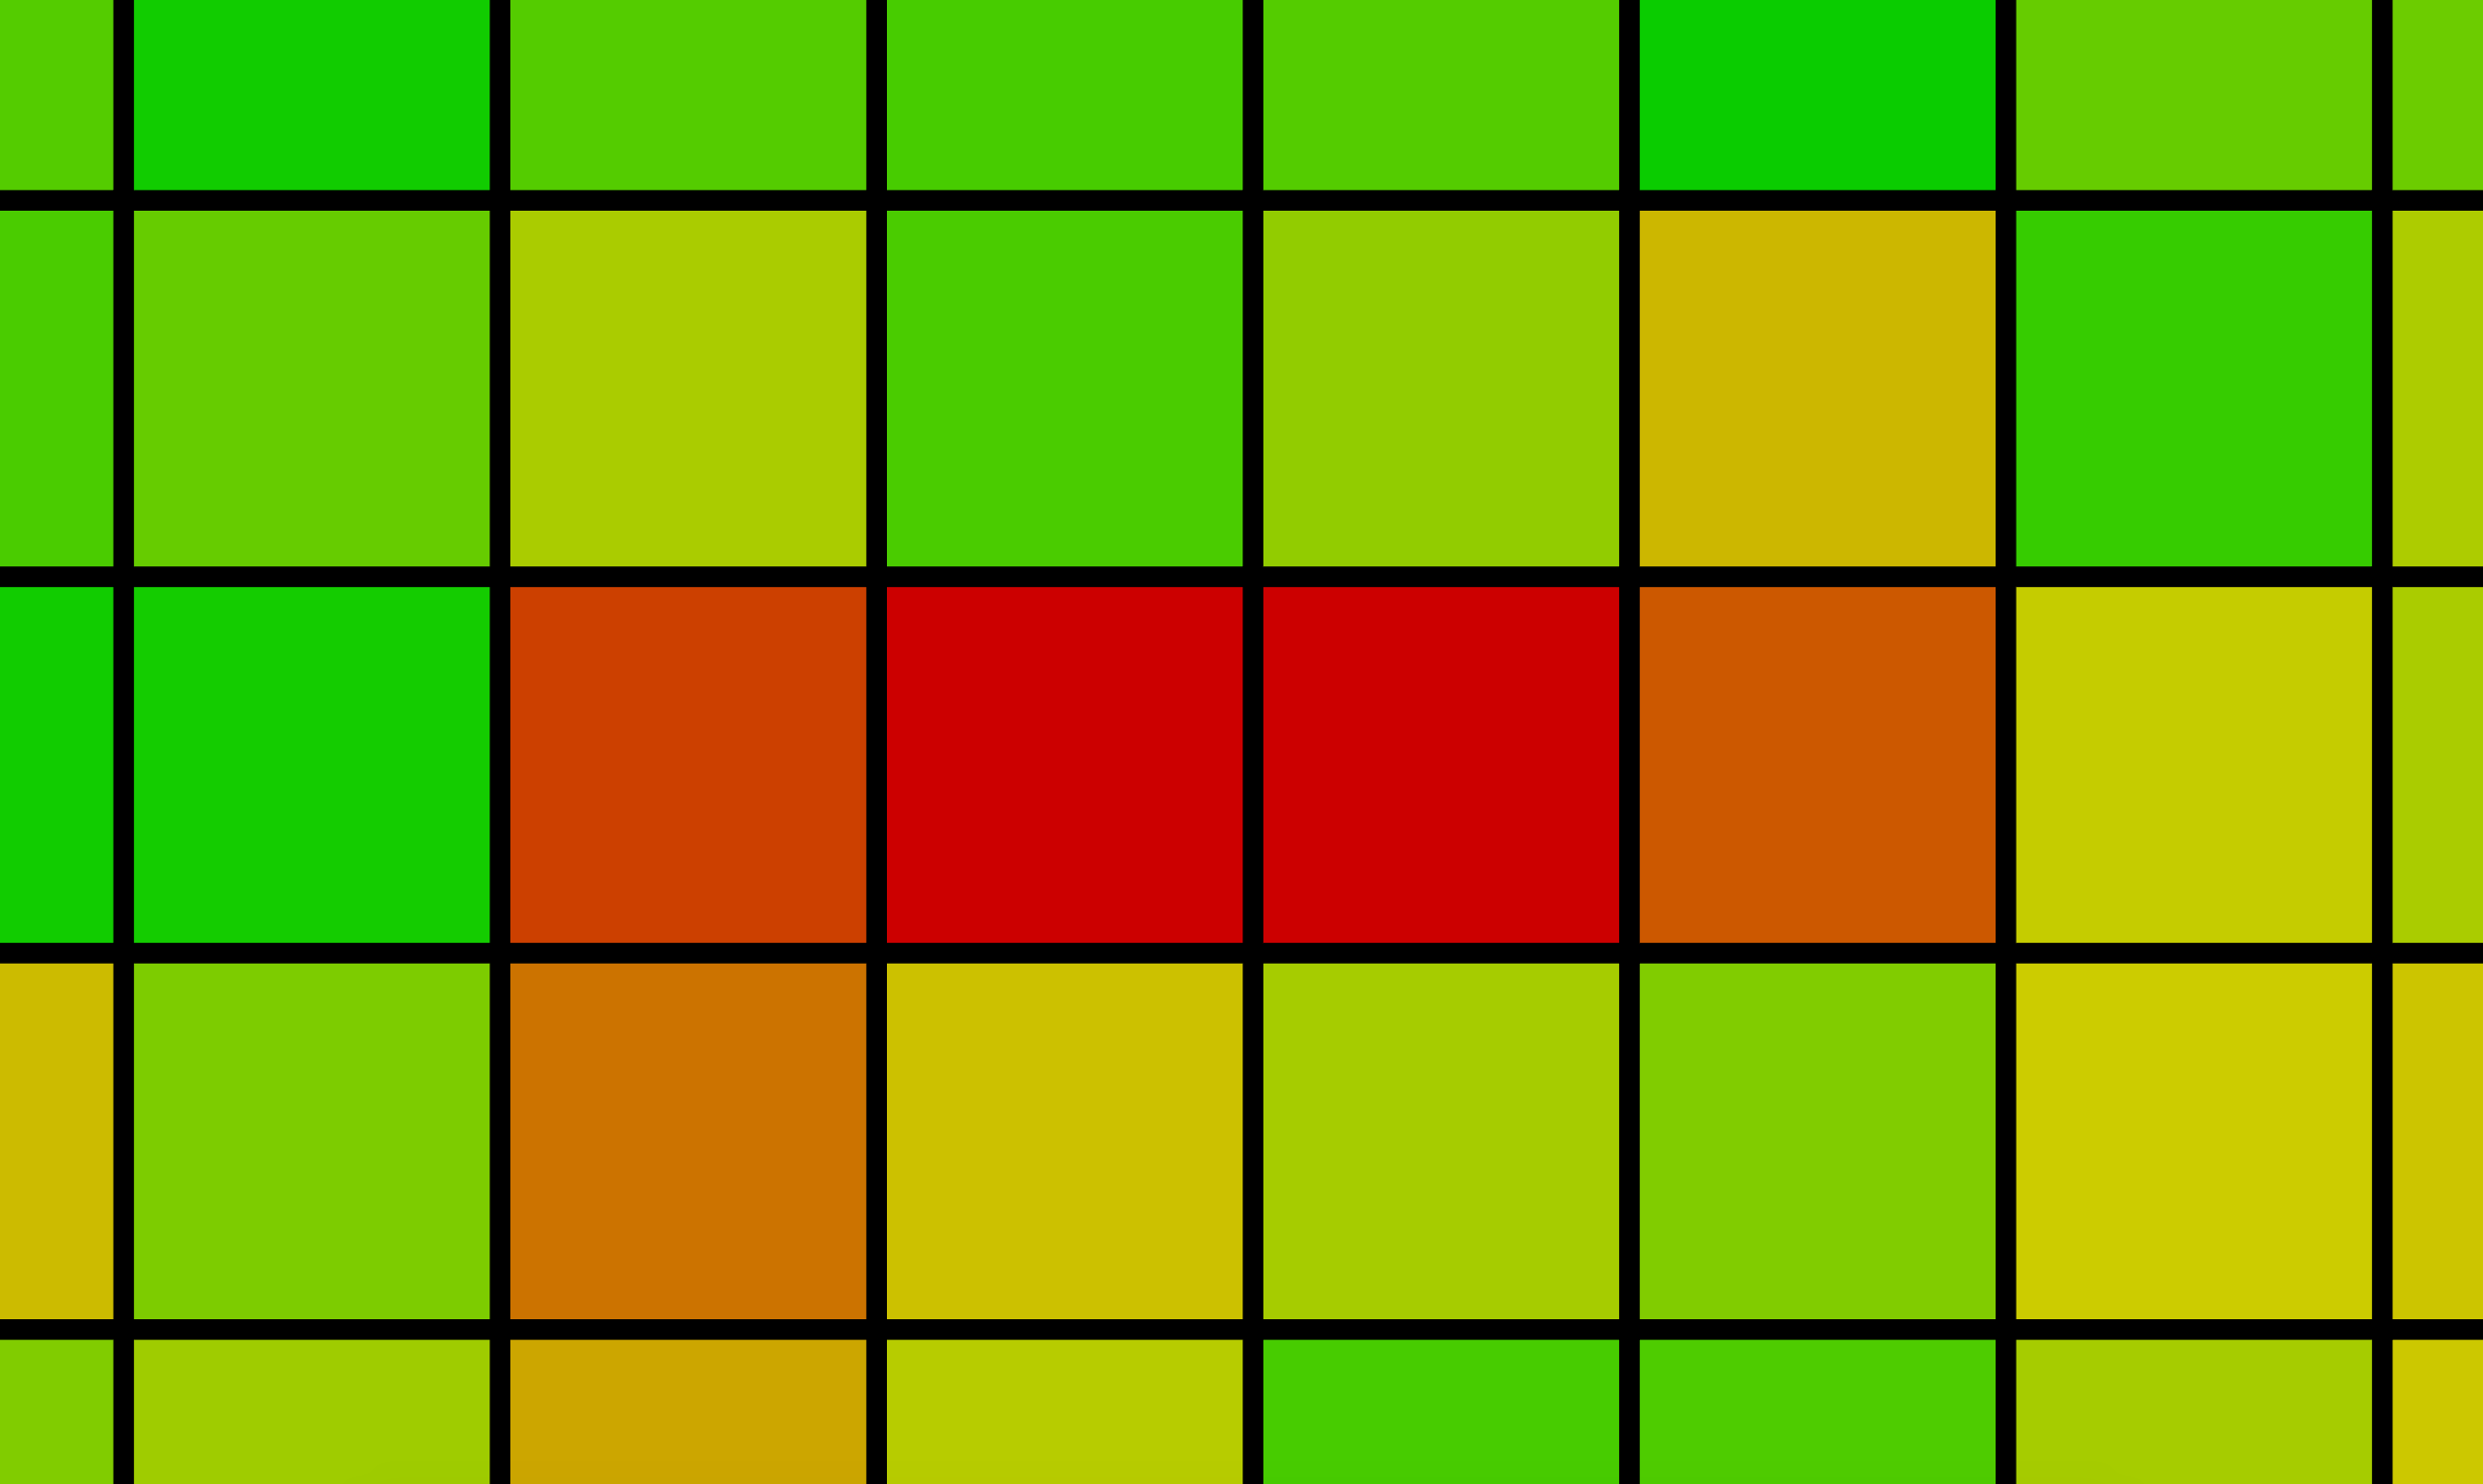
\includegraphics[width=0.5\textwidth]{Images/vis-edges-no.png}
    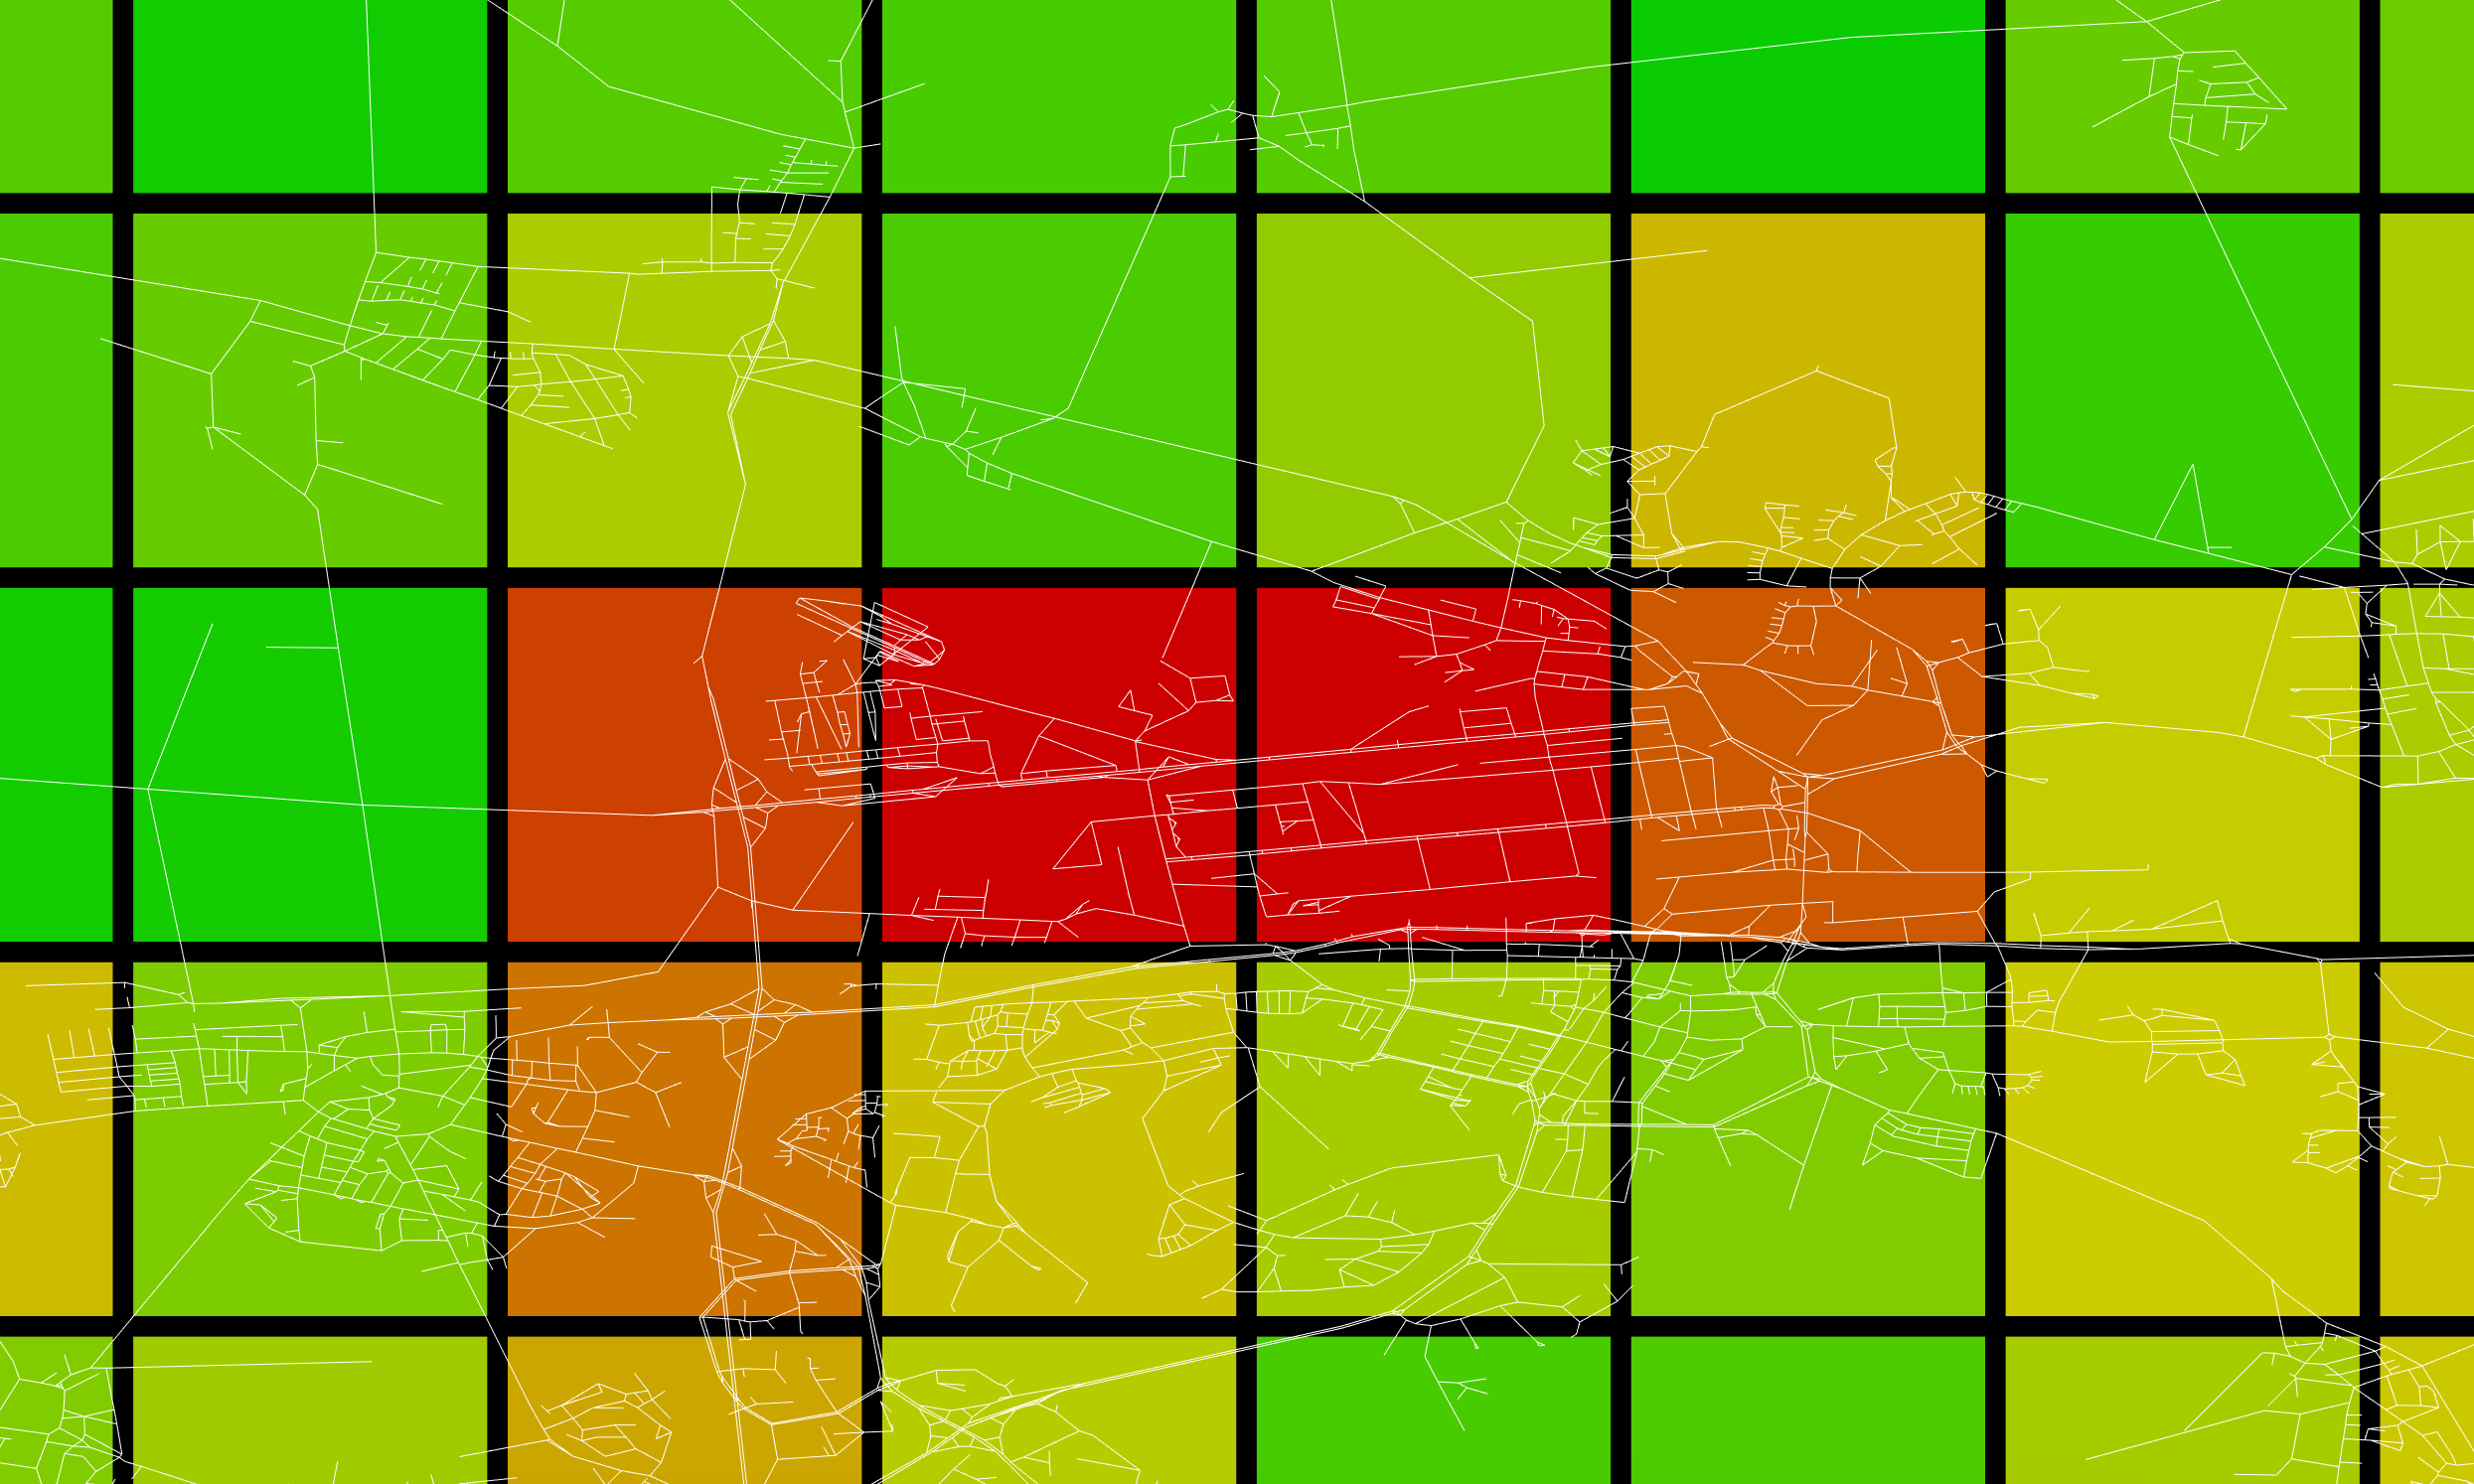
\includegraphics[width=0.5\textwidth]{Images/vis-edges-white.png}
\caption[]{Viewing the graph itself in addition to the tiles.}
\label{fig:white edges}
\end{figure}

Showing the edges helps to understand why some tiles in \cref{fig:white edges} are loaded more often than others.
The tiles with more reloadings have a high amount of nodes and edges.
Nevertheless, there are also other tiles with many nodes and edges, which are loaded less often.
Therefore we decided to use the colored edges described in \cref{graph} and thereby also include information about the speed.

\begin{figure}[H]
    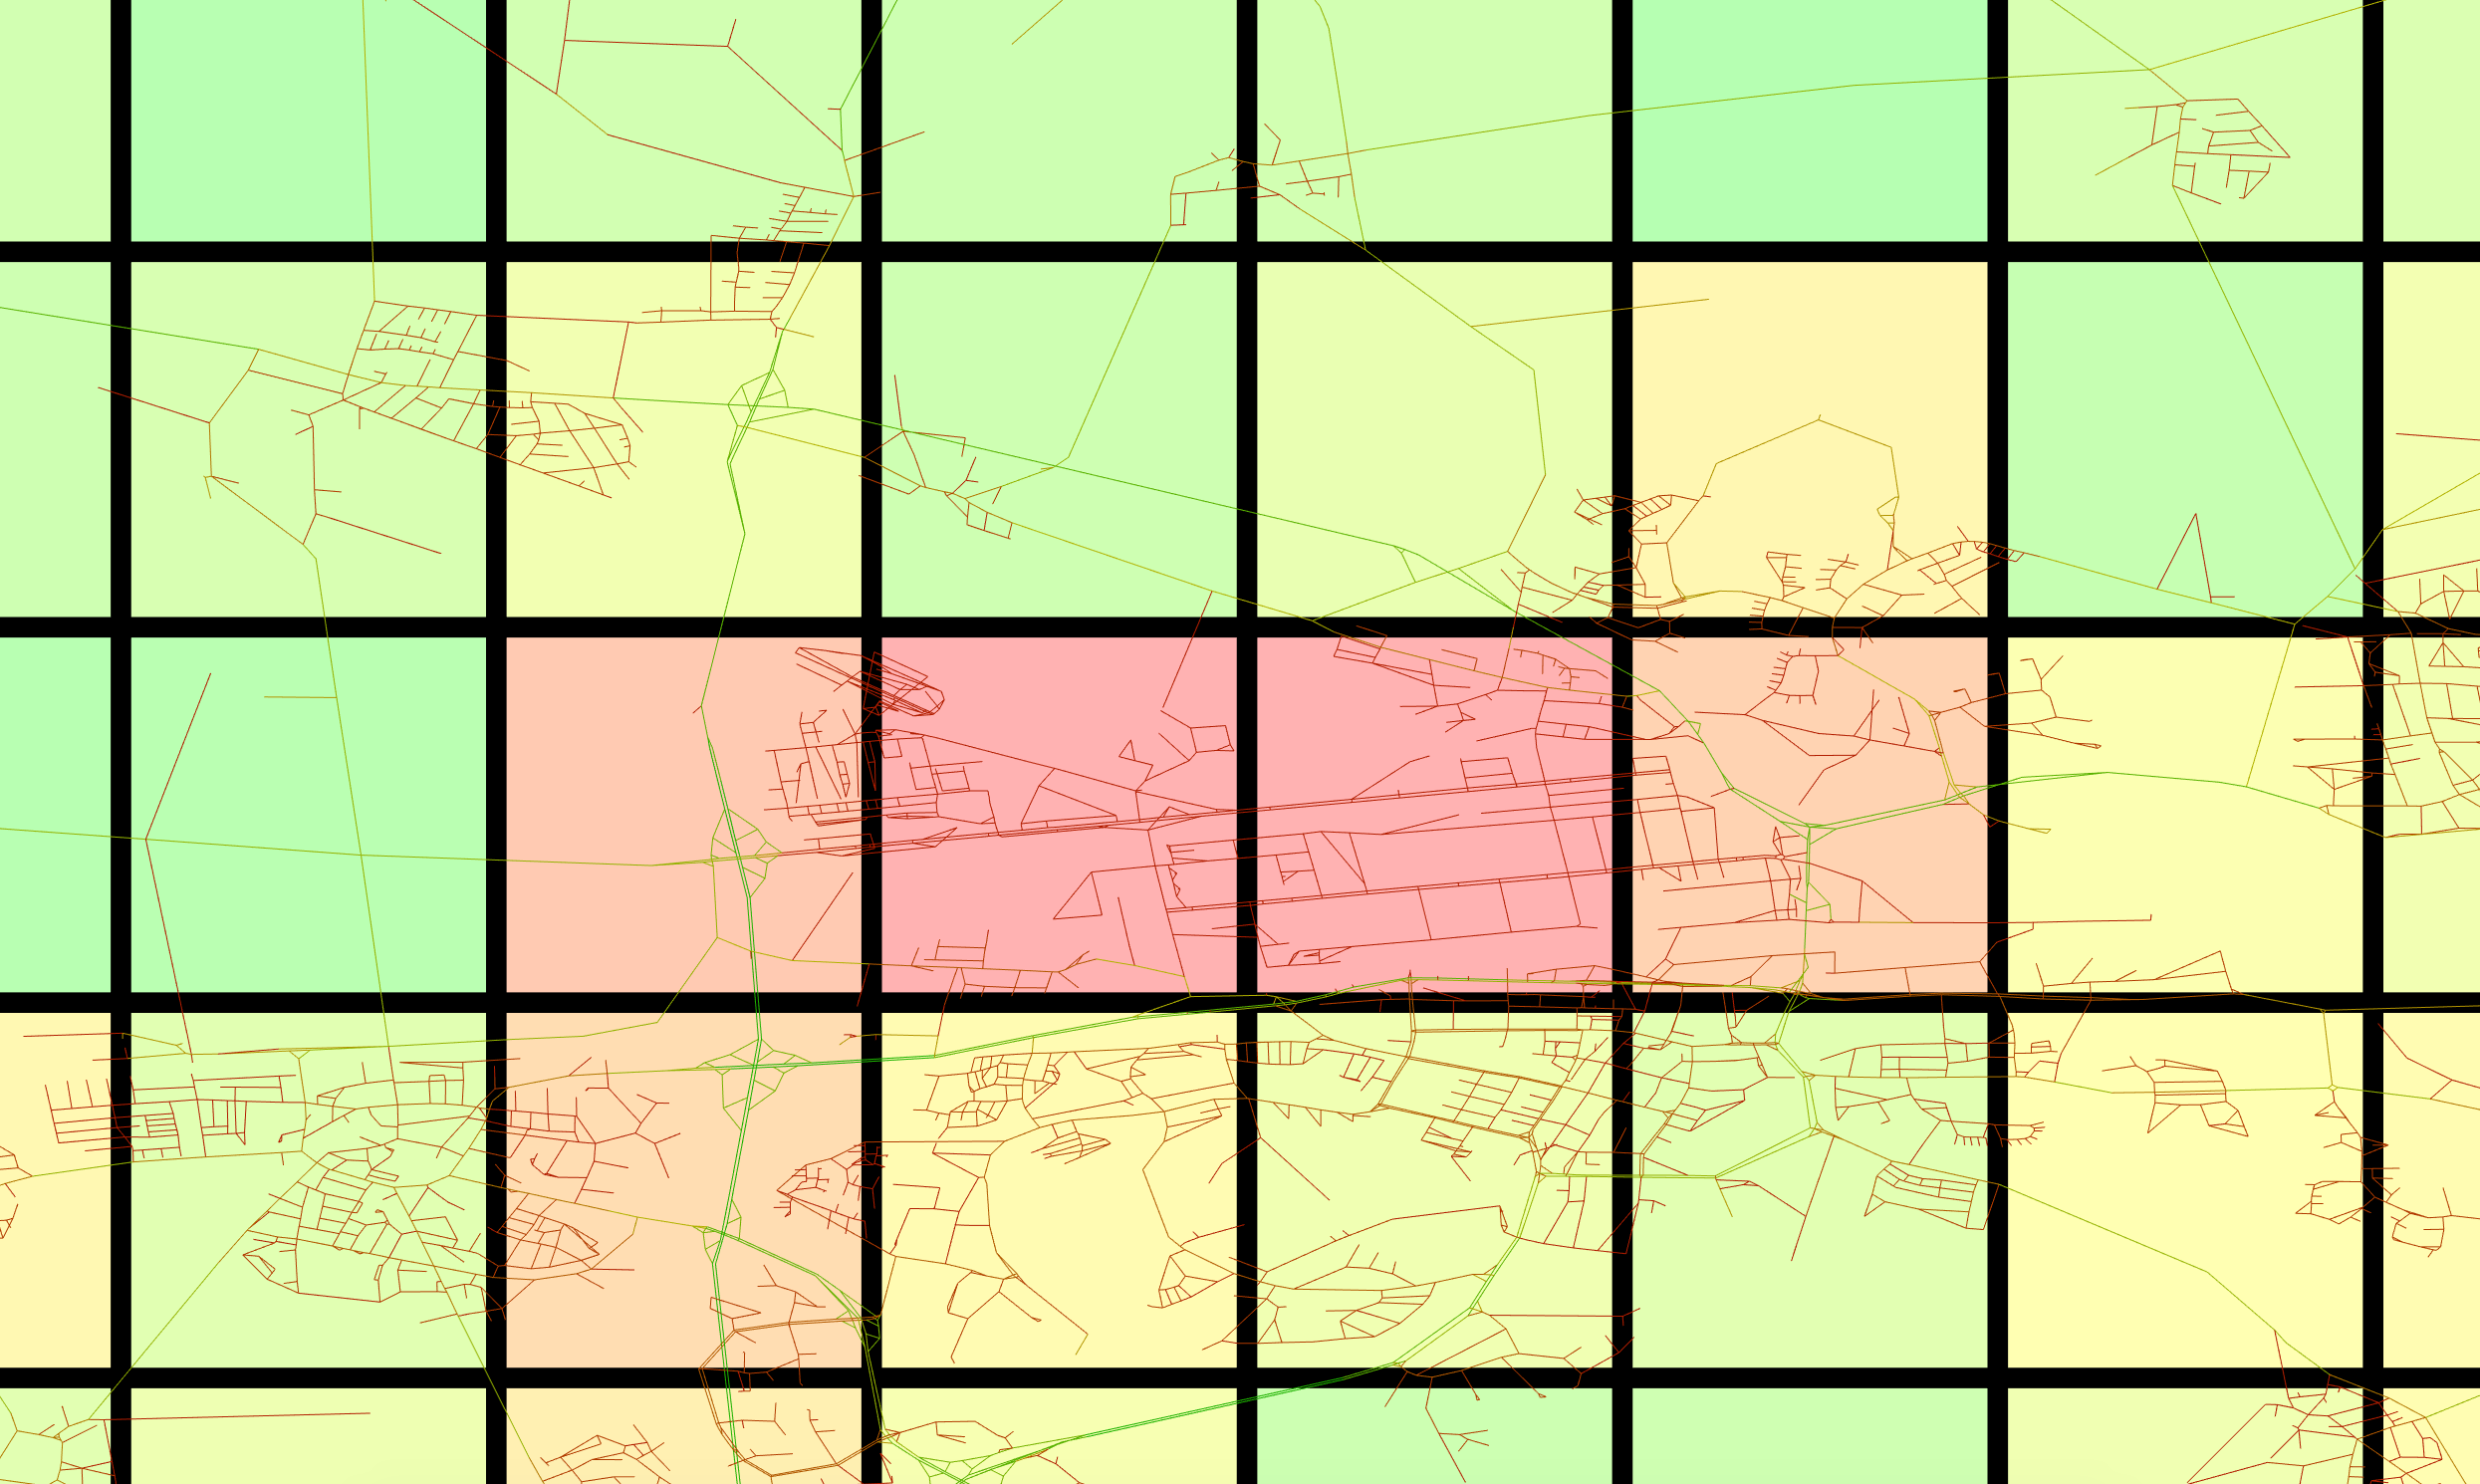
\includegraphics[width=\textwidth]{Images/vis-edges-hsv.png}
\caption[]{Speed based color scheeme. The background had to become a little brighter, when the edges are shown as it would be hard to recognize them clearly. }
\label{fig:colored edges}
\end{figure}

In \cref{fig:colored edges} we can now see that in the tiles that are loaded more often there are not only many edges, but those with a very small speed.
The surrounding and less loaded tiles allow a higher speed in general.

An other feature we needed, after the framework became better was to be able to adjust the level of coloring reloaded, as it is otherwise not possible to find the tiles that have been loaded more often when the most loaded tiles have only been loaded 5 times.
We decided to make this level adjustable while the visualization is running.

\begin{figure}[H]
    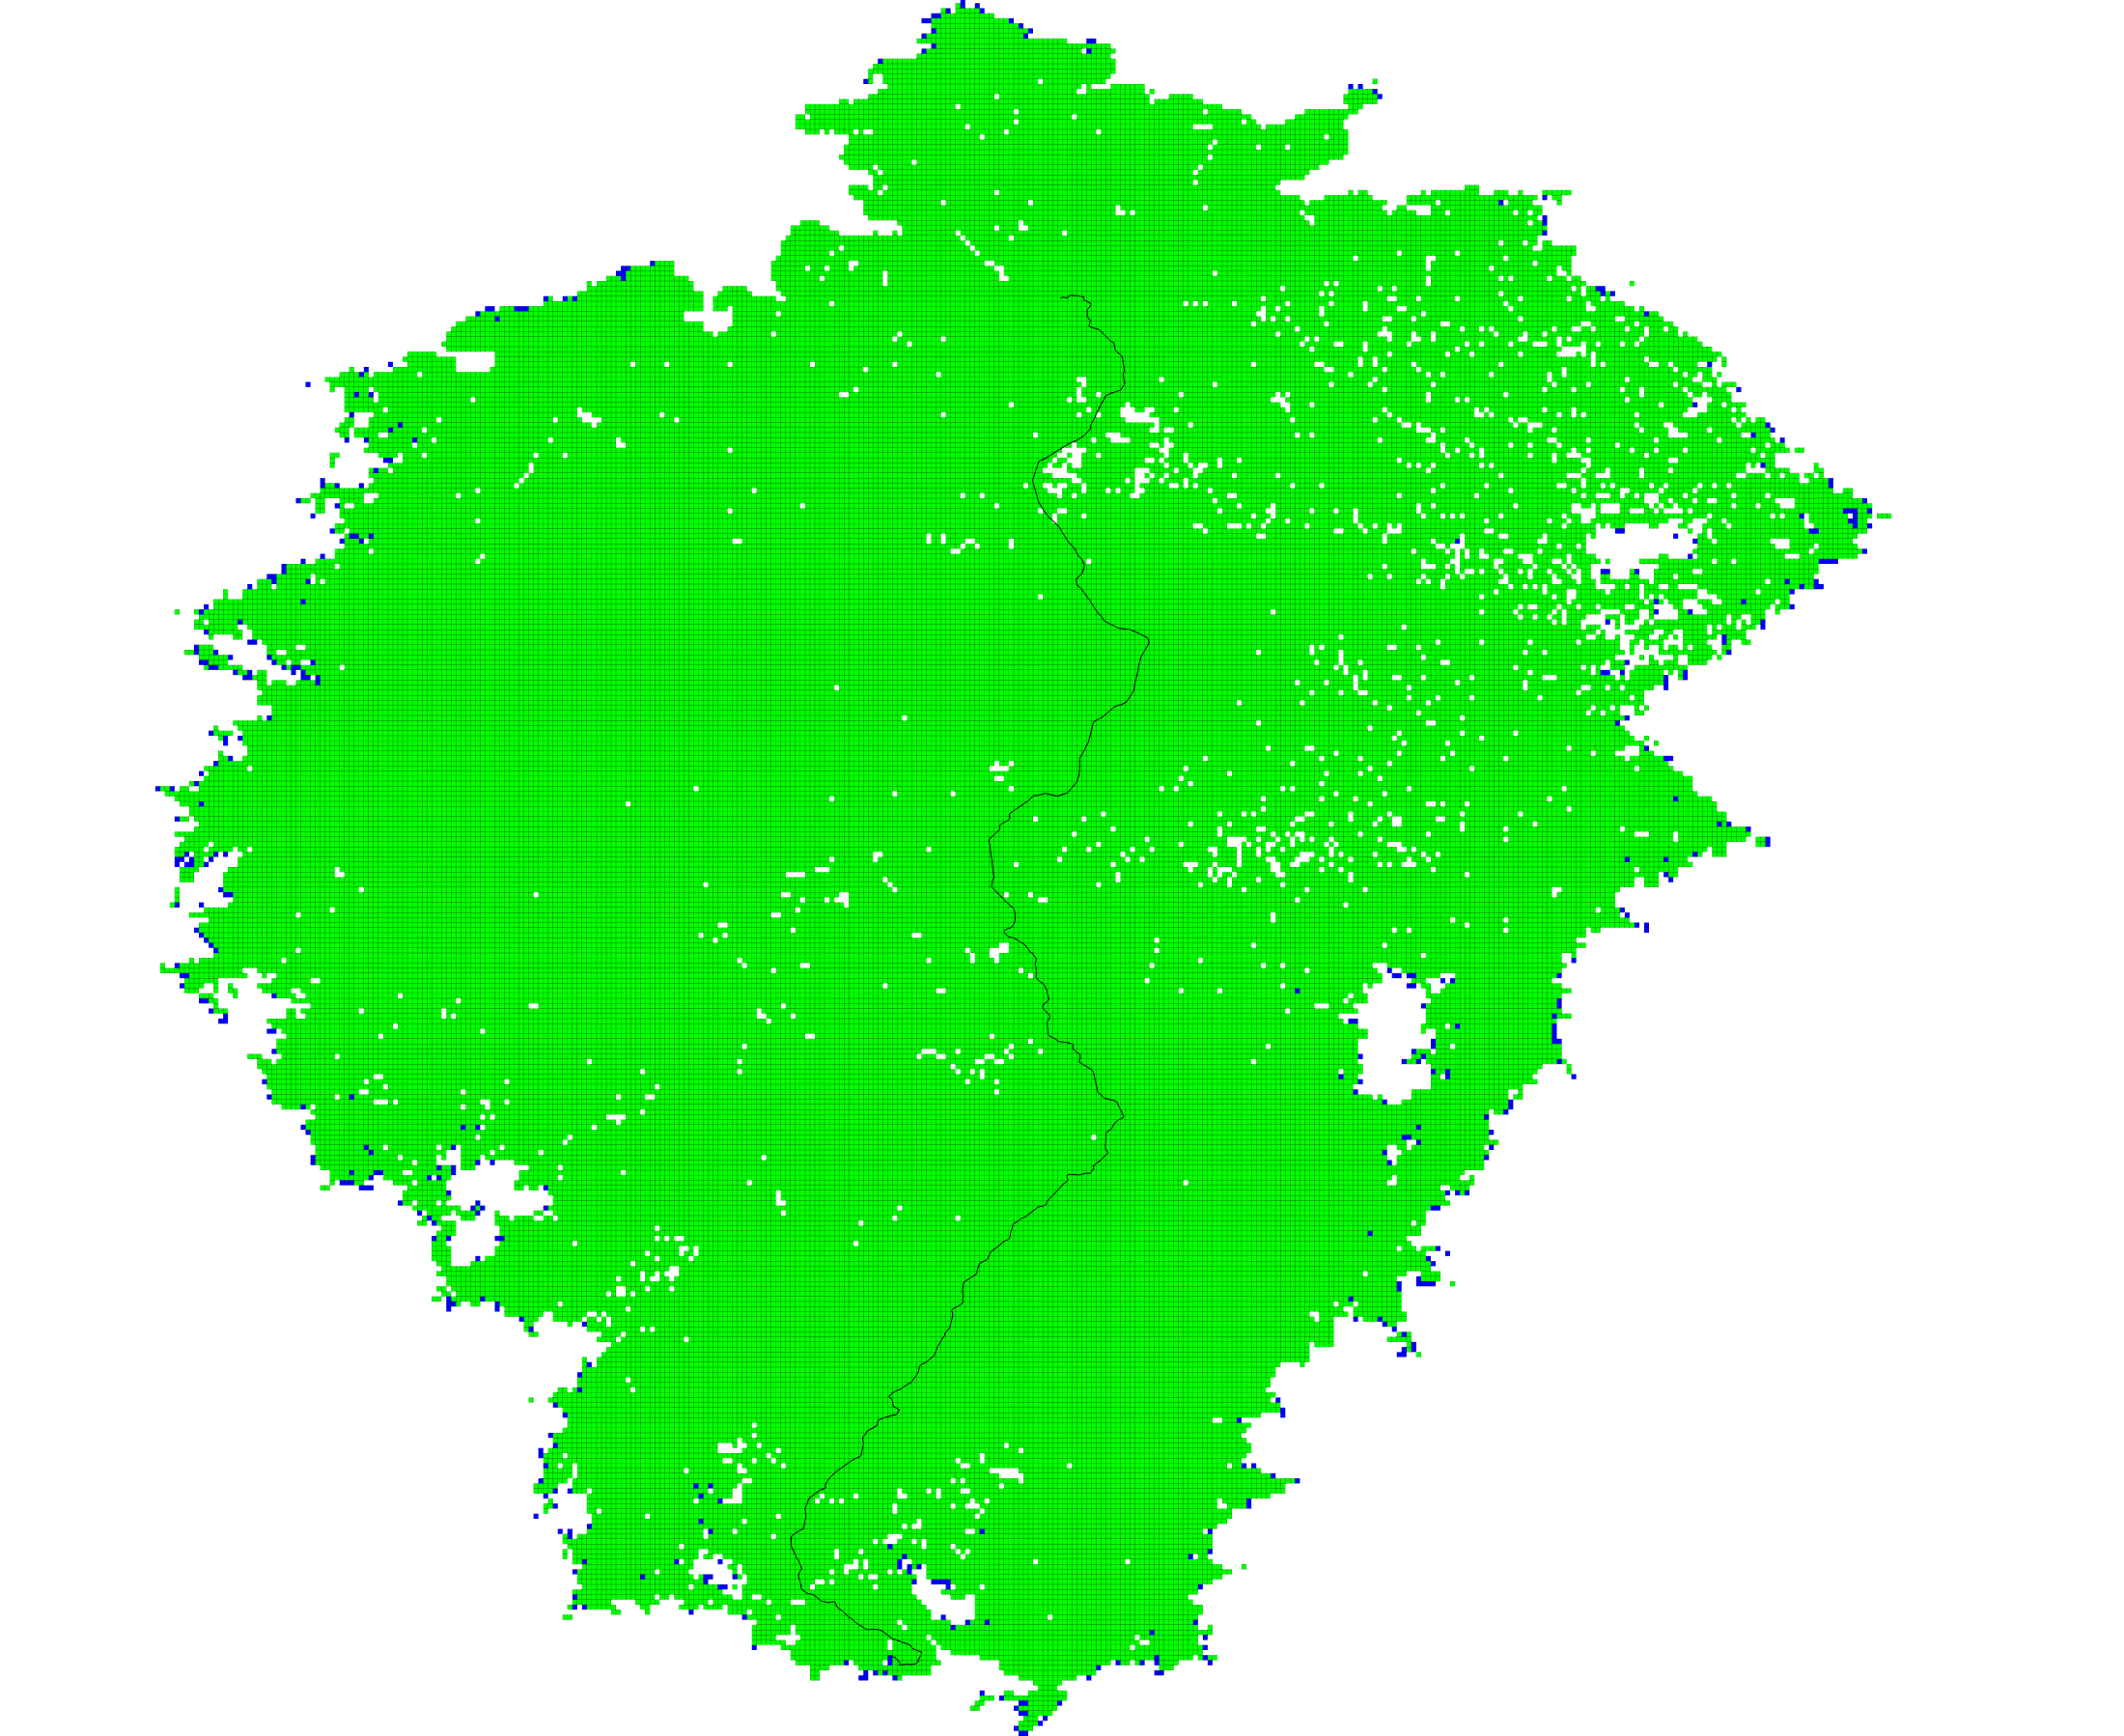
\includegraphics[width=0.5\textwidth]{Images/vis-no-factor.png}
  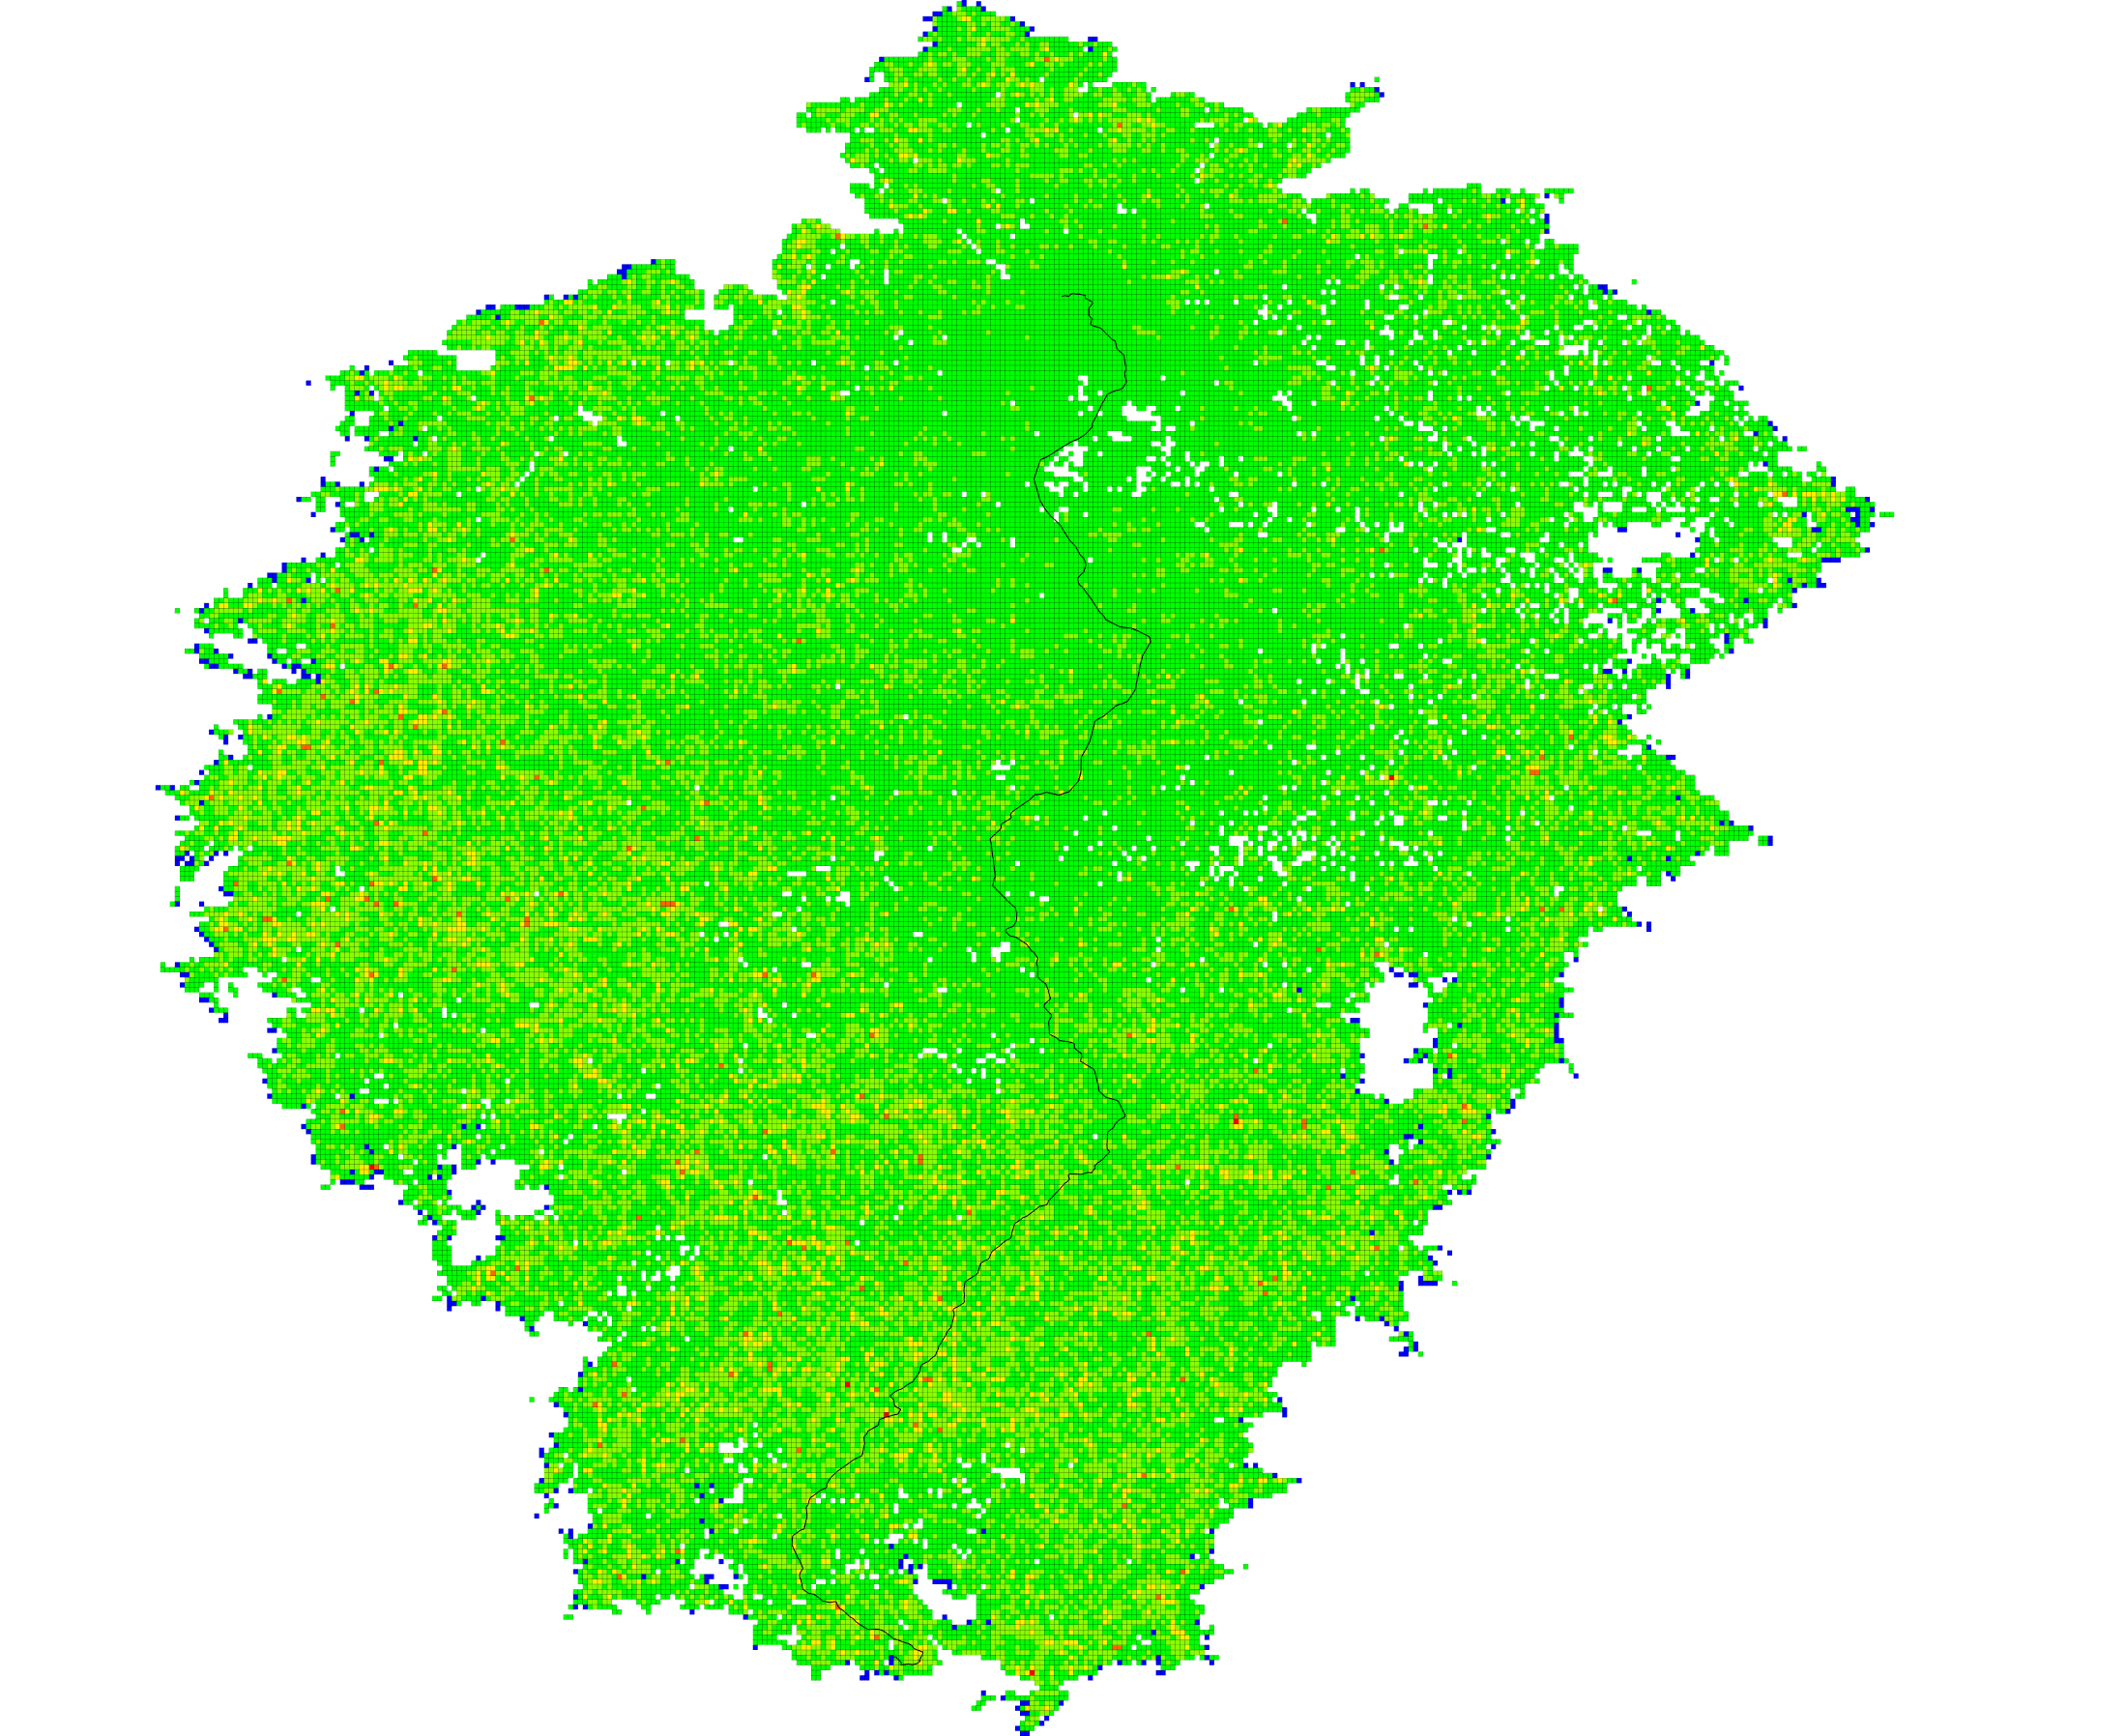
\includegraphics[width=0.5\textwidth]{Images/vis-factor.png}
\caption[]{A }
\label{fig:factor}
\end{figure}

By increasing the coloring of reloads in \cref{factor} we are now able to recognize weaknesses even on highly developed versions of the framework.


\chapter{Outlook}
\begin{itemize}
    \item verschiedene Projektionen
    \item knoten anordnen mit kanten mit länge = kosten
    \item different layers
    \item gerichtete edges
\end{itemize}

% References
\renewcommand*{\bibname}{References}
\bibliographystyle{abbrvnat}
\bibliography{Files/References}


\chapter*{Independence Declaration}
\addcontentsline{toc}{chapter}{Declaration of Authorship}
\thispagestyle{empty}

I hereby declare that the thesis submitted is my own unaided work. All direct or indirect sources used are acknowledged as references.\vspace{2 ex}

Potsdam, \today\\[6 ex]

\begin{flushleft}
    \begin{tabular}{p{5cm}}
        \hline
        \centering\footnotesize\printAuthor
    \end{tabular}
\end{flushleft}


\end{document}
